    \documentclass{article}

\usepackage{cancel}
\usepackage{tikz}
\usepackage{amsmath}
\usepackage{geometry}
\usepackage{graphicx}
\usepackage{amsfonts} 
\usepackage{verbatim}
\usepackage{mathrsfs}  
\usepackage{lmodern}
\usepackage{braket}
\usepackage{steinmetz}
\usepackage{bookmark}
\usepackage{pgfplots}
\pgfplotsset{compat=1.16}

\hypersetup{
    colorlinks=true,
    linkcolor=black,
}
\tikzset{block/.style = {draw, fill=white, very thick, rectangle, minimum height=1cm, minimum width=2cm},  
         square/.style = {draw, fill=white, very thick, rectangle, minimum height=1cm, minimum width=1cm},
         sum/.style= {draw, fill=white, very thick, circle, node distance=0.5cm},  
         cross/.pic = {  \draw[rotate = 45] (-#1,0) -- (#1,0);
                         \draw[rotate = 45] (0,-#1) -- (0, #1);}}


\renewcommand{\contentsname}{Indice}

\numberwithin{equation}{subsection}

\title{Appunti di Fondamenti di Telecomunicazioni}
\author{Giacomo Sturm}
\date{AA: 2023/2024 - Ing. Informatica}

\begin{document}

\maketitle

\vspace{10mm}

\begin{center}
    Sorgente del file LaTeX disponibile su \url{https://github.com/00Darxk/Fondamenti-di-Telecomunicazioni}
\end{center}

\clearpage

\tableofcontents

\clearpage

\section{Introduzione}

Un segnale è definito come una qualsiasi grandezza fisica che varia nel tempo in maniera deterministica o aleatoria. Può essere un'onda di pressione come la voce, o un onda 
elettromagnetica come segnali wireless e bluetooth. Un segnale è in grado di contenere informazioni come una sequenza di bit. Generalmente un segnale 
analogico viene convertito in digitale come un segnale elettrico tramite un trasduttore, per facilitare la processazione, per poi essere riconvertito in analogico; alcuni 
segnali sono creati direttamente in digitale. Un segnale è definito dalla sua banda, o spettro di banda, che ne determina la capicità di trasmettere informazione. L' 
occupazione in frequenza di un segnale è analoga al numero di bit di un dato digitale. 



Un segnale comune è il segnale voce, definito da un'onda di pressione, per cui è sempre strettamente positivo. Questo segnale è analogico, quindi continuo, ed il suo valoro è 
noto in ogni istante di tempo $t$, e si identifica come $x(t)$. 

\begin{center}
    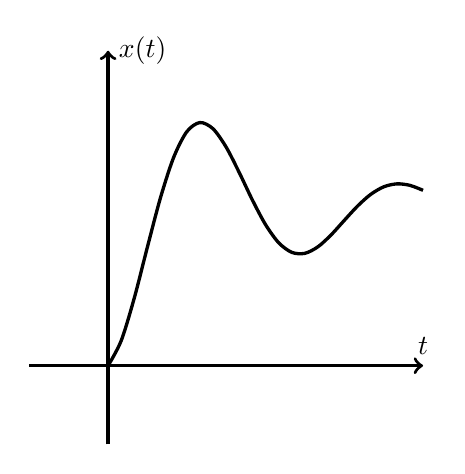
\begin{tikzpicture}[scale=2]
        \draw[->,very thick](-0.5,0)--(2,0)node[above]{$t$};
        \draw[->,very thick](0,-0.5)--(0,2)node[right]{$x(t)$};

        \draw[-,very thick]plot[smooth, domain=0:2](\x,{e^(-\x)*sin((5*\x-pi/2) r)+1});
    \end{tikzpicture}
\end{center}

Campionando un segnale anlogico si crea un segnale digitale, considerando prima alcune condizioni definite dal teroema del campionamento. Per campionare un segnale si estraggono
valori, o campioni, dal segnale analogico ogni intervallo $T$. Il segnale così ottenuto è un segnale discreto $x_n$ o $x[n]$, che presenta un valore ogni multiplo del tempo di campionamenoto $T$ 
scelto. 
\begin{equation*}
    x[n]:=\{x(n\cdot T)\,\forall n\in\mathbb{N}\}
\end{equation*}

\begin{center}
    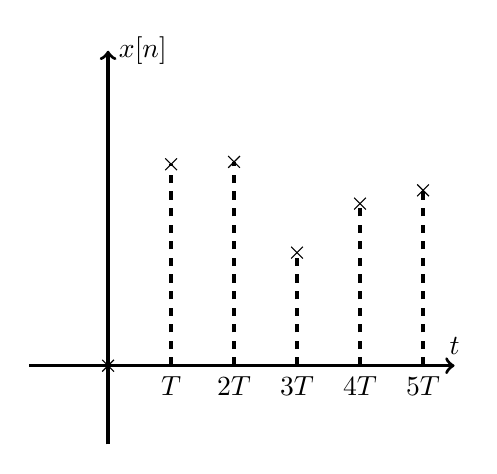
\begin{tikzpicture}[scale=2]
        \draw[->,very thick](-0.5,0)--(2.2,0)node[above]{$t$};
        \draw[->,very thick](0,-0.5)--(0,2)node[right]{$x[n]$};        

        \draw(0,0)pic[black]{cross=3pt};
        \draw(0.4,1.279)pic[black]{cross=3pt};
        \draw(0.8,1.294)pic[black]{cross=3pt};
        \draw(1.2,0.718)pic[black]{cross=3pt};
        \draw(1.6,1.0294)pic[black]{cross=3pt};
        \draw(2,1.1136)pic[black]{cross=3pt};

        \draw[dashed,very thick](0.4,0)node[below]{$T$}--(0.4,1.279);
        \draw[dashed,very thick](0.8,0)node[below]{$2T$}--(0.8,1.294);
        \draw[dashed,very thick](1.2,0)node[below]{$3T$}--(1.2,0.718);
        \draw[dashed,very thick](1.6,0)node[below]{$4T$}--(1.6,1.0294);
        \draw[dashed,very thick](2,0)node[below]{$5T$}--(2,1.1136);
    \end{tikzpicture}
\end{center}

Questi valori vengono poi convertiti in digitale assegnando un certo numero di bit per rappresentare l'intervallo massimo di valori descritti dal segnale. Questo processo 
viene chiamato quantizzazione, si divide l'intervallo dei valori in piccoli intervalli ognuno con un univoco valore in bit, in modo da convertire tutti i valori in quell'
intervallo in una sequenza di bit. Aumentando il numero di bit, quindi il numero di suddivisioni dell'itnervallo di partenza, aumenta la precisione, ma aumenta anche il costo 
per processare lo stesso segnale. Dopo aver covnertito tutti i valori in una sequenza di bit, questo segnale in bit viene tramesso, ed in seguito decodificato in analogico. 
Spesso i segnali vengono creati in digitale, per cui non è necessario campionare un segnale analogico. 


Campionando un segnale si perdono le informazioni contenute tra i campioni, ma è possibile applicare fitri e trasformazioni in digitale utili da giustificare la questa perdita 
di informazioni, per cui la maggior parte dei segnali vengono trasmessi in digitale. 




I segnali possono essere classificati in certi (deterministici) o aleatori (non deterministici). I segnali certi sono segnali di cui è noto tutto l'andamento, come file salvati su un supporto, per cui non è necessario 
trasmetterli. Mentre i segnali aleatori non sono noti a priori e vengono studiati dal punto di vista della statistica. 

In generale un sistema di trasmissione di segnali è formato da un trasmettitore che processa e codifica il segnale, un canale che lo trasmette, ed un ricevitore che lo decodifica:
\begin{center}
    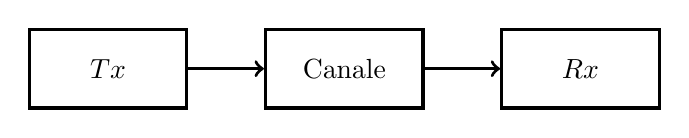
\begin{tikzpicture}[scale=2]
        \node[block](tx)at(-0.5,0){$Tx$};
        \node[block](rx)at(2.5,0){$Rx$};
        \node[block](c)at(1,0){Canale};
        \draw[->,very thick](tx.0)--(c.180);
        \draw[->,very thick](c.0)--(rx.180);
    \end{tikzpicture}
\end{center}

\clearpage

\section{Segnali a Tempo Continuo}

Vengono definiti in questa sezione una serie di segnali canonici, e le operazioni attuabili su questo tipo di segnali:

\subsection{Seno Cardinale}

\begin{equation}
    x(t)=\mbox{sinc}(t):=\displaystyle\frac{\sin(\pi t)}{\pi t}
\end{equation}
Questo segnale si attenua asintoticamente come $1/t$: 
\begin{equation*}
    \displaystyle-\frac{1}{t}\leq\mbox{sinc}(t)\leq\frac{1}{t}
\end{equation*}
Viene incluso il fattore $\pi$ nell'argomento in modo che la funzione si annulli per ogni valore intero:
\begin{equation*}
    \mbox{sinc}(t)=0\,\forall t\in\mathbb{Z}
\end{equation*}

\begin{center}
    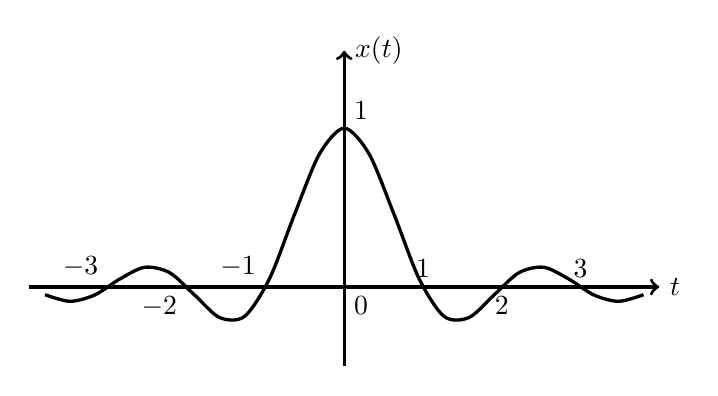
\begin{tikzpicture}[scale=2]
        \draw[->,very thick](0,-0.5)--(0,1.5)node[right]{$x(t)$};
        \draw[->,very thick](-2,0)--(2,0)node[right]{$t$};
        \draw[-,very thick]plot[smooth, domain=-1.9:1.9](\x,{1/(2*pi*\x)*sin(2*pi*\x r)});
        \node[above right]at(0,1){$1$};
        \node[above]at(0.5,0){$1$};
        \node[below]at(1,0){$2$};
        \node[above]at(1.5,0){$3$};
        \node[above left]at(-0.5,0){$-1$};
        \node[below left]at(-1,0){$-2$};
        \node[above left]at(-1.5,0){$-3$};
        \node[below right]at(0,0){$0$};

    \end{tikzpicture}
\end{center}

\subsection{Coseno}

\begin{equation}
    x(t)=\cos\left(\displaystyle\frac{2\pi t}{T}\right)
\end{equation}

Il parametro $T$ rappresenta il periodo della funzione, per cui il valore della funzione ad un certo valore $t$ corrisponde al valore in $t-T$. Invece del periodo si può 
usare la frequenza $f_0$, inverso del periodo. 

\begin{center}
    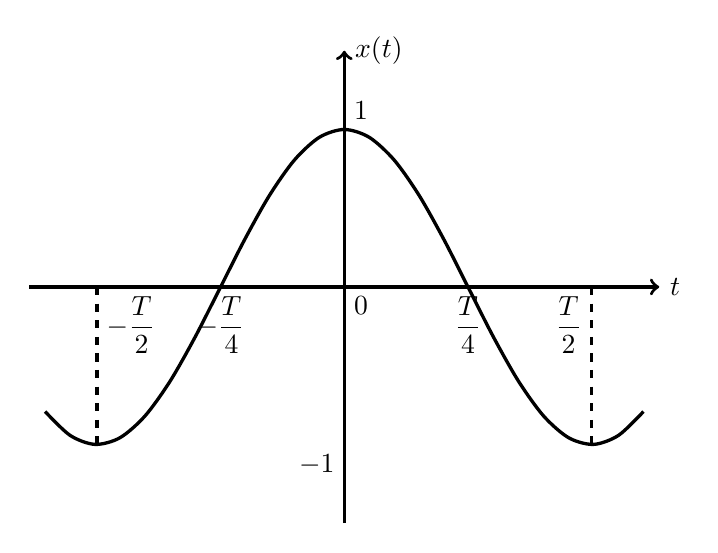
\begin{tikzpicture}[scale=2]
        \draw[->,very thick](0,-1.5)--(0,1.5)node[right]{$x(t)$};
        \draw[->,very thick](-2,0)--(2,0)node[right]{$t$};   
        \draw[-,very thick]plot[smooth, domain=-1.9:1.9](\x,{cos(2*\x r)});
        
        \node[below]at(0.785,0){$\displaystyle\frac{T}{4}$};
        \node[below]at(-0.785,0){$\displaystyle-\frac{T}{4}$};
        \node[below left]at(1.5707,0){$\displaystyle\frac{T}{2}$};
        \node[below right]at(-1.5707,0){$\displaystyle-\frac{T}{2}$};
        \draw[dashed,very thick](1.5707,0)--(1.5707,-1);
        \draw[dashed,very thick](-1.5707,0)--(-1.5707,-1);
        \node[above right]at(0,1){$1$};
        \node[below left]at(0,-1){$-1$};
        \node[below right]at(0,0){$0$};
    \end{tikzpicture}
\end{center}

\subsection{Gradino Periodico o Onda Quadra}

\begin{center}
    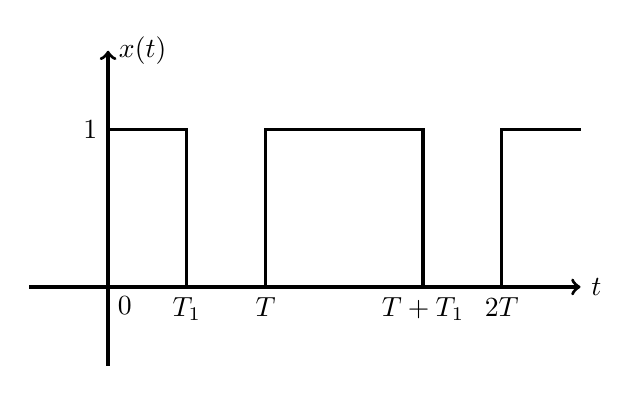
\begin{tikzpicture}[scale=2]
        \draw[->,very thick](-0.5,0)--(3,0)node[right]{$t$};
        \draw[->,very thick](0,-0.5)--(0,1.5)node[right]{$x(t)$};
        \node[below right]at(0,0){$0$};

        \draw[-,very thick](0,1)node[left]{$1$}--(0.5,1)--(0.5,0)node[below]{$T_1$}--(1,0)node[below]{$T$}--(1,1)--(2,1)--(2,0)node[below]{$T+T_1$}--(2.5,0)node[below]{$2T$}--(2.5,1)--(3,1);
    \end{tikzpicture}
\end{center}

\subsection{Esponenziale Complesso}

\begin{equation}
    x(t)=\displaystyle e^{i\frac{2\pi t}{T}}=\cos\left(\frac{2\pi t}{T}\right)+i\sin\left(\frac{2\pi t}{T}\right)
\end{equation}

Un segnale complesso può essere anlizzato mediante la sua fase ed il uso modulo in funzione del tempo:
\begin{equation*}
    x(t)=|x(t)|e^{\displaystyle\phase{x(t)}}
\end{equation*}

Dato che la fase è periodica si può rappresentare come una serie di rampe.

\begin{center}
    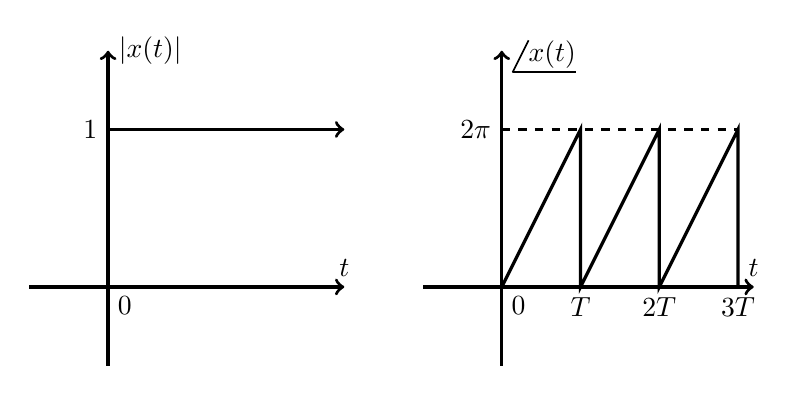
\begin{tikzpicture}[scale=2]
        \draw[->,very thick](-0.5,0)--(1.5,0)node[above]{$t$};
        \draw[->,very thick](0,1)node[left]{$1$}--(1.5,1);
        \draw[->,very thick](0,-0.5)--(0,1.5)node[right]{$|x(t)|$};
        \node[below right]at(0,0){$0$};

        \draw[->,very thick](2,0)--(4.1,0)node[above]{$t$};
        \draw[->,very thick](2.5,-0.5)--(2.5,1.5)node[right]{$\phase{x(t)}$};
        \draw[dashed,very thick](2.5,1)node[left]{$2\pi$}--(4,1);
        \node[below right]at(2.5,0){$0$};

        \draw[-,very thick](2.5,0)--(3,1)--(3,0)node[below]{$T$}--(3.5,1)--(3.5,0)node[below]{$2T$}--(4,1)--(4,0)node[below]{$3T$};
    \end{tikzpicture}
\end{center}

\subsection{Esponenziale}

\begin{equation}
    x(t)=e^{-\alpha t},\,\alpha\in\mathbb{R}
\end{equation}

\begin{center}
    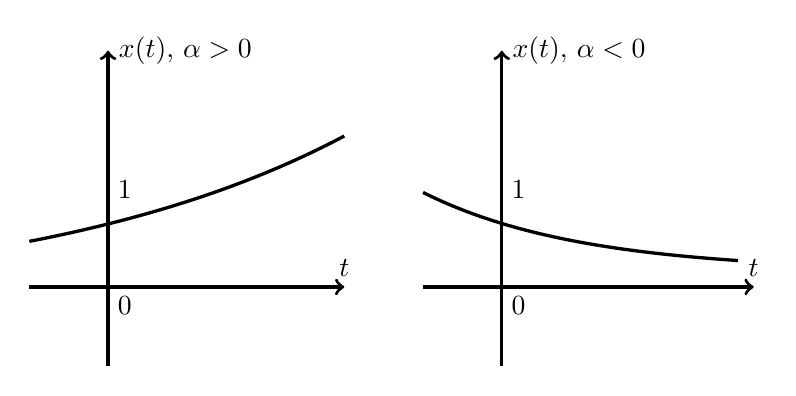
\begin{tikzpicture}[scale=2]
        \draw[->,very thick](-0.5,0)--(1.5,0)node[above]{$t$};
        \draw[->,very thick](0,-0.5)--(0,1.5)node[right]{$x(t),\,\alpha>0$};
        \draw[-,very thick]plot[smooth, domain=-0.5:1.5](\x,{1/2*e^(1/2*\x)-0.1});
        \node[above right]at(0,0.5){$1$};
        \node[below right]at(0,0){$0$};

        \draw[->,very thick](2,0)--(4.1,0)node[above]{$t$};
        \draw[->,very thick](2.5,-0.5)--(2.5,1.5)node[right]{$x(t),\,\alpha<0$};
        \draw[-,very thick]plot[smooth, domain=2:4](\x,{1/2*e^(-(\x-2))+0.1});
        \node[above right]at(2.5,0.5){$1$};
        \node[below right]at(2.5,0){$0$};
    \end{tikzpicture}
\end{center}

\subsection{Finestra}

\begin{equation}
    x(t)=\mbox{rect}\left(\displaystyle\frac{t}{T}\right):=\begin{cases}
        1 & \displaystyle-\frac{T}{2}\leq t <\frac{T}{2}\\
        0 & \displaystyle t<-\frac{T}{2} \land t\geq\frac{T}{2}
    \end{cases}
\end{equation}

$T$ viene chiamata base della finestra. Questo segnale presenta una discontinuità di salto per $t=\pm\displaystyle\frac{1}{2}$. La funzione finestra viene usata quando si 
vuole analizzare solo una parte di un segnale, poiché il restante sarà pari a $0$. La trasformata di questa funzione rappresenta un filtro in frequenza. 

\begin{center}
    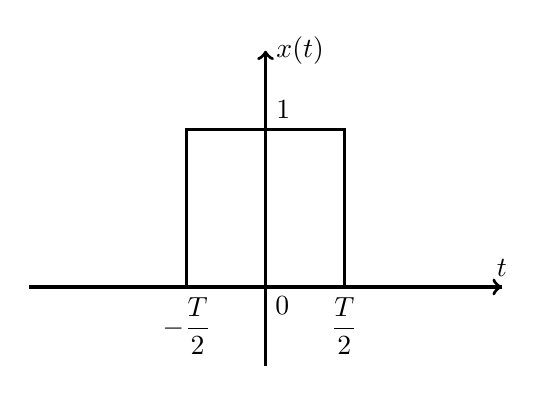
\begin{tikzpicture}[scale=2]
        \draw[->,very thick](-1.5,0)--(1.5,0)node[above]{$t$};
        \draw[->,very thick](0,-0.5)--(0,1.5)node[right]{$x(t)$};
        \node[below right]at(0,0){$0$};

        \draw[-,very thick](-1.5,0)--(-0.5,0)node[below]{$\displaystyle-\frac{T}{2}$}--(-0.5,1)--(0,1)node[above right]{$1$}--(0.5,1)--(0.5,0)node[below]{$\displaystyle\frac{T}{2}$}--(1.5,0);        
    \end{tikzpicture}
\end{center}

\subsection{Triangolo}

\begin{equation}
    x(t)=\mbox{tri}\left(\displaystyle\frac{t}{T}\right):=\begin{cases}
        1-|t| & -T\leq t < T\\
        0 & t<-T \land t\geq T
    \end{cases}
\end{equation}

\begin{center}
    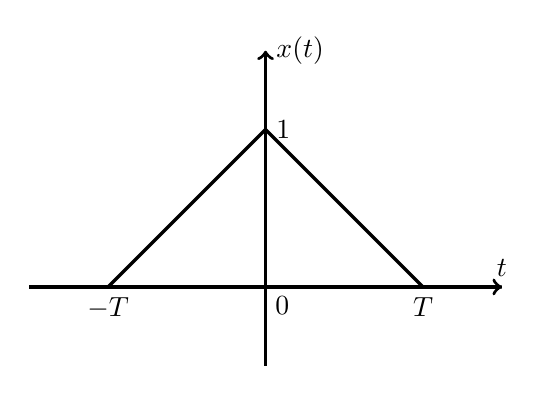
\begin{tikzpicture}[scale=2]
        \draw[->,very thick](-1.5,0)--(1.5,0)node[above]{$t$};
        \draw[->,very thick](0,-0.5)--(0,1.5)node[right]{$x(t)$};
        \node[below right]at(0,0){$0$};

        \draw[-,very thick](-1.5,0)--(-1,0)node[below]{$-T$}--(0,1)node[right]{$1$}--(1,0)node[below]{$T$}--(1.5,0);
    \end{tikzpicture}
\end{center}

\subsection{Gradino}

\begin{equation}
    x(t)=u(t):=\begin{cases}
        1 & t\geq0\\
        0 & t<0
    \end{cases}
\end{equation}

\begin{center}
    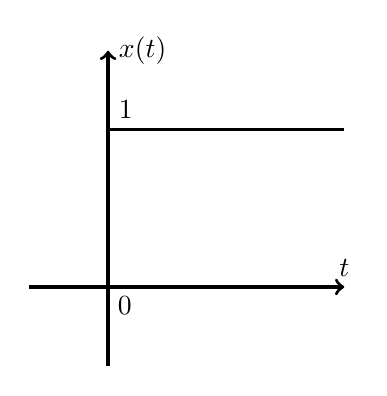
\begin{tikzpicture}[scale=2]
        \draw[->,very thick](-0.5,0)--(1.5,0)node[above]{$t$};
        \draw[->,very thick](0,-0.5)--(0,1.5)node[right]{$x(t)$};
        \draw[-,very thick](-0.5,0)--(0,0)--(0,1)node[above right]{$1$}--(1.5,1);
        \node[below right]at(0,0){$0$};
    \end{tikzpicture}
\end{center}

\subsection{Gaussiana}

\begin{equation*}
    x(t)=e^{-\alpha t^2}\,\,\alpha\in\mathbb{R}^+
\end{equation*}

La larghezza della campana centrale dipende dal fattore $\alpha$. Nello sturio delle probabiltà, si usa la sua forma normalizzata:
\begin{equation*}
    x(t)=\displaystyle\frac{e^{-\frac{t^2}{2\sigma^2}}}{\sqrt{2\pi}\sigma}
\end{equation*}
Il valore $\sigma$ rappresenta la deviazione standard, mentre il suo quadrato $\sigma^2$ descrive la varianza. 

\begin{center}
    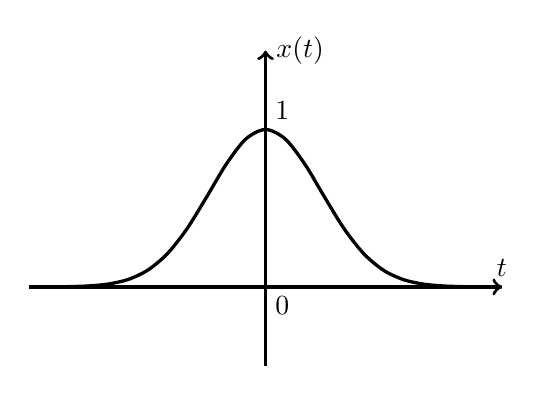
\begin{tikzpicture}[scale=2]
        \draw[->,very thick](-1.5,0)--(1.5,0)node[above]{$t$};
        \draw[->,very thick](0,-0.5)--(0,1.5)node[right]{$x(t)$};
        \node[below right]at(0,0){$0$};
        \node[above right]at(0,1){$1$};


        \draw[-,very thick]plot[smooth, domain=-1.5:1.5](\x,{e^(-(2*\x)^2)});
    \end{tikzpicture}
\end{center}

\subsection{Esponenziale Unilatero}

\begin{equation*}
    x(t)=e^{-\alpha t}\cdot u(t)\,\,\alpha\in\mathbb{R}^+
\end{equation*}

\begin{center}
    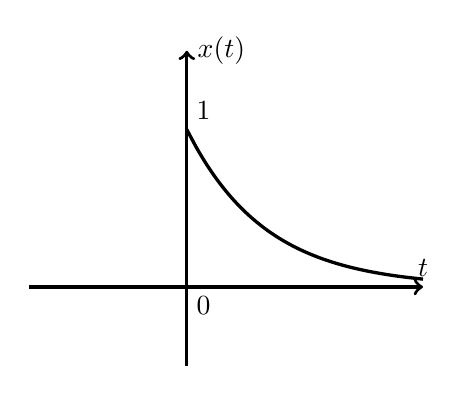
\begin{tikzpicture}[scale=2]
        \draw[->,very thick](-1,0)--(1.5,0)node[above]{$t$};
        \draw[->,very thick](0,-0.5)--(0,1.5)node[right]{$x(t)$};
        \node[below right]at(0,0){$0$};
        \node[above right]at(0,1){$1$};

        \draw[-,very thick](-1,0)--(0,0);
        \draw[-,very thick]plot[smooth, domain=0:1.5](\x,{e^(-2*(\x))});
    \end{tikzpicture}
\end{center}

\subsection{Costante}

\begin{equation*}
    x(t)=a
\end{equation*}

\begin{center}
    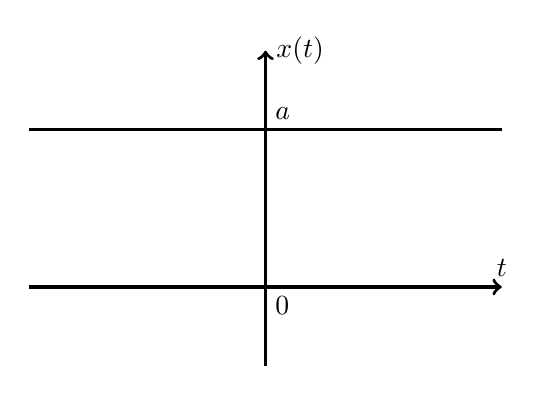
\begin{tikzpicture}[scale=2]
        \draw[->,very thick](-1.5,0)--(1.5,0)node[above]{$t$};
        \draw[->,very thick](0,-0.5)--(0,1.5)node[right]{$x(t)$};
        \node[below right]at(0,0){$0$};
        \node[above right]at(0,1){$a$};

        \draw[-,very thick](-1.5,1)--(1.5,1);
    \end{tikzpicture}
\end{center}

\subsection{Segno}

\begin{equation*}
    x(t)=\mbox{sign}(t):=\begin{cases}
        1&t>0\\
        -1&t<0
    \end{cases}
\end{equation*}

\begin{center}
    \begin{tikzpicture}[scale=2]
        \draw[->,very thick](-1.5,0)--(1.5,0)node[above]{$t$};
        \draw[->,very thick](0,-1.5)--(0,1.5)node[right]{$x(t)$};
        \node[below right]at(0,0){$0$};
        \node[above right]at(0,1){$1$};
        \node[below left]at(0,-1){$-1$};

        \draw[-,very thick](0,1)--(1.5,1);
        \draw[-,very thick](0,-1)--(-1.5,-1);
    \end{tikzpicture}
\end{center}

\subsection{Operazioni sui Segnali}

Le operazioni sui segnali vengono computate istante per istante. L'operazione di somma produce un segnale $z(t)$, tale che ogni valore che assume equivale alla somma 
di altri due segnali $x(t)$ e $y(t)$ nello stesso istante:
\begin{equation*}
    z(t)=x(t)+y(t)
\end{equation*}

Analogamente si considera l'operazione prodotto, come un prodotto istante per istante tra i due segnali:
\begin{equation*}
    z(t)=x(t)\cdot y(t)
\end{equation*}

L'operazione di ribaltamento corrisponde ad una riflessione della funzione lungo l'asse delle ascisse di un segnale $x(t)$ tramite una sostituzione di variabile $t\to-t$:
\begin{equation*}
    z(t)=x(-t)
\end{equation*}
Quest'operazione non produce risultati per segnali pari, poiché presentano la proprietà $x(t)=x(-t)$. 
Tramite l'operazione di ribaltamento si può esprimere il segnale segno tramite la differenza di due gradini:
\begin{equation*}
    \mbox{sign}(t)=u(t)-u(-t)
\end{equation*}


L'operazione di traslazione, sposta un segnale $x(t)$ lungo l'asse delle ascisse di un fattore $\tau$:
\begin{equation*}
    z(t)=x(t-\tau)
\end{equation*}

L'operazione di cambio di scale corrisponde ad un rimpicciolimento o allargamento di un segnale $x(t)$ di un fattore $a\in\mathbb{R}$:
\begin{equation*}
    z(t)=x(at)
\end{equation*}

\subsection{Energia e Potenza}

L'energia e la potenza di un segnale rappresentano caratteristiche utili nella loro analisi e processazione. 

Viene definita energia $E_x$ di un segnale $x(t)$, come il limite per $\Delta t\to0$ di un integrale:
\begin{equation}
    E_x:=\lim_{\Delta t\to\infty}\displaystyle\int_{-\frac{\Delta t}{2}}^{\frac{\Delta t}{2}}|x(t)|^2dt=\int_{-\infty}^{\infty}|x(t)|^2dt
\end{equation}
L'energia di un segnale è sempre strettamente positiva, poiché si considera tutta l'area sottesa dal quadrato del modulo del segnale, necessariamente positivo; mentre è nulla 
solo se lo è anche il segnale analizzato. Teoricamente non esiste un limite per l'energia contenuta in un segnale, ma sono fisicamente realizzabile solo segnali con energia 
finita e non infinita. 

Se l'energia di un segnale è finita e diversa da zero $E_x\neq\infty$ e $E_x\neq0$, il segnale $x(t)$ si chiama segnale di energia.


Viene definita la potenza $P_x$ di un segnale $x(t)$ in maniera simile alla sua energia:
\begin{equation}
    P_x:=\lim_{\Delta t\to\infty}\displaystyle\left(\frac{1}{\Delta t}\int_{-\frac{\Delta t}{2}}^{\frac{\Delta t}{2}}|x(t)|^2dt\right)
\end{equation}
Anche la potenza di un segnale è strettamente positiva $P_x\geq0$, se la potenza assume valori diversi da zero e finiti, il segnale $x(t)$ si chiama segnale di potenza. 

Vengono così create due classi di segnali, di potenza e di energi. Per la definizione delle due grandezze antisimmetriche poiché se un segnale è di potenza, non è di energia 
e viceversa: 
\begin{gather*}
    E\implies\neg P\\
    P\implies\neg E
\end{gather*}

Si determina l'energia di una gaussiana di ampiezza $A$:
\begin{gather*}
    E_x=\lim_{\Delta t\to\infty}\displaystyle\int_{-\frac{\Delta t}{2}}^{\frac{\Delta t}{2}}A^2e^{-2\alpha t^2}dt=A^2\lim_{\Delta t\to\infty}\displaystyle\int_{-\frac{\Delta t}{2}}^{\frac{\Delta t}{2}}e^{-2\alpha t^2}dt
\end{gather*}
Si considera il cambio di variabile $\tau=\sqrt{2\alpha}t$:
\begin{equation*}
    E_x=A^2\lim_{\Delta t\to\infty}\displaystyle\int_{-\frac{\Delta t}{2}}^{\frac{\Delta t}{2}}\frac{e^{-\tau^2}}{\sqrt{2\alpha}}d\tau=\frac{A^2}{\sqrt{2\alpha}}\int_{-\infty}^{+\infty}e^{-\tau^2}d\tau
\end{equation*}

L'integrale ottenuto è l'integrale di Gauss, risolubile applicando un cambio di coordinate polari al quadrato dell'integrale dato, il risultato dell'integrazione della 
gaussiana sull'intero asse dei reali $\mathbb{R}$ corrisponde alla radice di pi greco: 
\begin{equation*}
    \displaystyle\int_{\mathbb{R}}e^{-t^2}dt=\sqrt\pi
\end{equation*}
Per cui l'energia di una gaussiana risulta essere:
\begin{equation}
    E_x=A^2\displaystyle\sqrt{\frac{\pi}{2\alpha}}
\end{equation}




Moltiplicando un segnale $x(t)$ moltiplicato per un gradino e calcolandone l'integrale sui tutti i reali $\mathbb{R}$, equivale all'integrale del segnale originiario sui soli 
reali positivi $\mathbb{R}^+$, poiché il segnale assume valori nulli da $-\infty$ a $0$: 
\begin{equation*}
    \displaystyle\int_{\mathbb{R}}x(t)\cdot u(t)dt=\int_{\mathbb{R}^+}x(t)dt
\end{equation*}



Si determina l'energia e la potenza di un esponenziale complesso. Il segnale ha un modulo unitario $|x(t)|=1$, per cui la sua energia risultante è:
\begin{equation*}
    E_x=\lim_{\Delta t\to\infty}\displaystyle\int_{-\frac{\Delta t}{2}}^{\frac{\Delta t}{2}}dt=\lim_{\Delta t\to\infty}\left(\frac{\Delta t}{2}+\frac{\Delta t}{2}\right)=\infty
\end{equation*}
Per cui l'esponenziale complesso non è un segnale di energia. La potenza risulta essere:
\begin{equation*}
    P_x=\lim_{\Delta t\to\infty}\displaystyle\left(\frac{1}{\Delta t}\int_{-\frac{\Delta t}{2}}^{\frac{\Delta t}{2}}dt\right)=\lim_{\Delta t\to\infty}\left(\frac{1}{\Delta t}\cdot\Delta t\right)=1
\end{equation*}
L'esponenziale complesso è quindi un segnale di potenza. 



Si determina l'energia di un esponenziale unilatero:
\begin{equation*}
    E_x=\displaystyle\int_{\mathbb{R}^+}e^{-2\alpha t}dt=\frac{1}{2\alpha}
\end{equation*}
Per cui questo segnale non è né di energia né di potenza. 


I segnali periodici non possono essere di energia, per cui un segnale perdiodico senza attenuazione non è fisicamente realizzabile. Quindi possono essere solo di potenza, 
si determina la potenza di un segnale periodico:
\begin{equation*}
    P_x=\lim_{\Delta t\to\infty}\displaystyle\left(\frac{1}{\Delta t}\int_{-\frac{\Delta t}{2}}^{\frac{\Delta t}{2}}|x(t)|^2dt\right)
\end{equation*}
In un segnale periodico si può esprimere l'intervallo di tempo $\Delta t$ come $n$ volte il periodo $T$:
\begin{equation*}
    P_x=\lim_{n\to\infty}\displaystyle\left(\frac{1}{n T}\int_{-\frac{nT}{2}}^{\frac{nT}{2}}|x(t)|^2dt\right)
\end{equation*}
L'integrale di un segnale perfettamente periodico, ovvero senza smorzamenti, su $n$ periodi equivale ad $n$ volte l'integrale su un singolo periodo $T$:
\begin{equation*}
    P_x=\lim_{n\to\infty}\displaystyle\left(\frac{1}{n T}n\int_{-\frac{n}{2}}^{\frac{T}{2}}|x(t)|^2dt\right)=\lim_{n\to\infty}\displaystyle\left(\frac{1}{T}\int_{-\frac{T}{2}}^{\frac{T}{2}}|x(t)|^2dt\right)
\end{equation*} 
Questo integrale è indipendente dalla variabile $n$, per cui si può trascurare il limite, la potenza risulta quindi essere:
\begin{equation}
    P_x=\displaystyle\frac{1}{T}\int_{-\frac{T}{2}}^{\frac{T}{2}}|x(t)|^2dt
\end{equation}
Quest'ultimo integrale può essere espresso in termini della frequenza naturale: $f_0=\frac{1}{T}$. 



Si determina la potenza del segnale coseno, di ampiezza $A$ e frequenza naturale $f_0$ $A\cos\left(2\pi f_0t\right)$:
\begin{equation*}
    P_x=\displaystyle A^2f_0\int_{-\frac{1}{2f_0}}^{\frac{1}{2f_0}}\cos^2(2\pi f_0 t)dt
\end{equation*}
Per esprimere il quadrato del coseno, si consdira la formula di bisezione del coseno:
\begin{gather*}
    \cos(2x)=2\cos^2(x)-1\\
    \cos^2(x)=\displaystyle\frac{\cos(2x)+1}{2}\\
    A^2\cos^2(2\pi f_0t)=\displaystyle\frac{A^2}{2}(\cos(4\pi f_0t)+1)
\end{gather*}
Si può esprimere inoltre mediante la notazione complessa delle funzioni trigonometriche:
\begin{gather*}
    A\cos(2\pi f_0t)=\displaystyle\frac{A}{2}(e^{i2\pi f_0t}+e^{-i2\pi f_0t})\\
    |x+y|^2\,\,x,y\in\mathbb{C}\\
    (x+y)\cdot(x+y)^*=(x+y)\cdot(x^*+y^*)\\
    xx^*+xy^*+yx^*+yy^*=|x|^2+|y|^2+xy^*+yx^*\\
    xy^*+yx^*=(a_x+ib_x)\cdot(a_y-ib_y)+(a_x-ib_x)\cdot(a_y+ib_y)=(a_xa_y+b_xb_y)=2Re\{x^*y\}\\
    |x|^2+|y|^2+2Re\{|x|e^{-\varphi_x}+|y|e^{i\varphi_y}\}\\
    |x|^2+|y|^2+2|x||y|\cos(|\varphi_y-\varphi_x|)\\
    \Bigg|\displaystyle\frac{A}{2}(e^{i2\pi f_0t}+e^{-i2\pi f_0t})\Bigg|^2=\frac{A^2}{4}\left(1+1+2Re\Bigl\{e^{i2\pi f_0t}\cdot\left(e^{-i2\pi f_0t}\right)^*\Bigr\}\right)\\
    A^2\cos^2(2\pi f_0t)=\displaystyle\frac{A^2}{2}(1+\cos(4\pi f_0t))
\end{gather*}
Considerando questa sostituzione, l'integrale diventa:
\begin{equation*}
    P_x=\displaystyle\frac{A^2f_0}{2}\int_{-\frac{1}{2f_0}}^{\frac{1}{2f_0}}(\cancelto{0}{\cos(4\pi f_0 t)}+1)dt=\frac{A^2f_0}{2}\left(\frac{1}{2f_0}+\frac{1}{2f_0}\right)=\frac{A^2}{2}
\end{equation*}
L'integrale su un periodo del coseno è nullo, poiché è una funzione pari, per cui la componente $\cos(4\pi f_0 t)$ fornisce un contributo nullo. 

\section{Segnali a Tempo Discreto}

Poiché la maggior parte dei segnali vengono trasmessi o generati in tempo discreto, è necessario essere a conoscenza del comportamento dei segnali continui campionati a 
tempo discreto. 

\subsection{Gradino}

\begin{equation*}
    x[n]=u[n]:=\begin{cases}
        1&n\geq0\\
        0&n<0
    \end{cases}
\end{equation*}

\begin{center}
    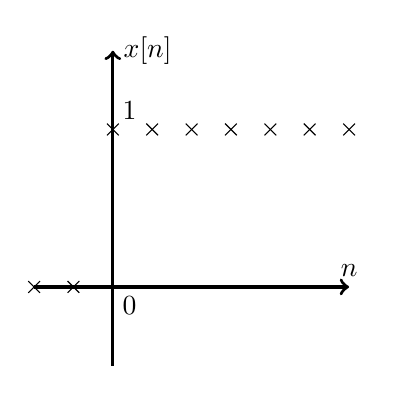
\begin{tikzpicture}[scale=2]
        \draw[->,very thick](-0.5,0)--(1.5,0)node[above]{$n$};
        \draw[->,very thick](0,-0.5)--(0,1.5)node[right]{$x[n]$};
        \draw(-0.5,0)pic[black]{cross=3pt};
        \draw(-0.25,0)pic[black]{cross=3pt};
        \draw(0,1)pic[black]{cross=3pt};
        \draw(0.25,1)pic[black]{cross=3pt};
        \draw(0.5,1)pic[black]{cross=3pt};
        \draw(0.75,1)pic[black]{cross=3pt};
        \draw(1,1)pic[black]{cross=3pt};
        \draw(1.25,1)pic[black]{cross=3pt};
        \draw(1.5,1)pic[black]{cross=3pt};

        \node[above right]at(0,1){$1$};
        \node[below right]at(0,0){$0$};
    \end{tikzpicture}
\end{center}

Non avendo un segnale finestra a tempo discreto, essa può essere descritta come la differenza di due gradini discreti. Una finestra di base $2l$ nel discreto si esprime come:
\begin{equation*}
    u[n+l]-u[n-(l+1)]
\end{equation*}

\begin{center}
    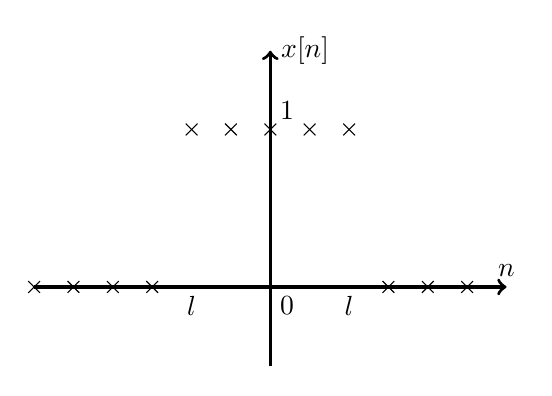
\begin{tikzpicture}[scale=2]
        \draw[->,very thick](-1.5,0)--(1.5,0)node[above]{$n$};
        \draw[->,very thick](0,-0.5)--(0,1.5)node[right]{$x[n]$};

    
        \draw(-1.5,0)pic[black]{cross=3pt};
        \draw(-1.25,0)pic[black]{cross=3pt};
        \draw(-1,0)pic[black]{cross=3pt};
        \draw(-0.75,0)pic[black]{cross=3pt};
        \draw(-0.5,1)pic[black]{cross=3pt};
        \draw(-0.25,1)pic[black]{cross=3pt};
        \draw(0,1)pic[black]{cross=3pt};
        \draw(0.25,1)pic[black]{cross=3pt};
        \draw(0.5,1)pic[black]{cross=3pt};
        \draw(0.75,0)pic[black]{cross=3pt};
        \draw(1,0)pic[black]{cross=3pt};
        \draw(1.25,0)pic[black]{cross=3pt};

        \node[below]at(-0.5,0){$l$};
        \node[below]at(0.5,0){$l$};
        \node[above right]at(0,1){$1$};
        \node[below right]at(0,0){$0$};
    \end{tikzpicture}
\end{center}

\subsection{Esponenziale Unilatero}

\begin{equation*}
    x[n]=a^nu[n]
\end{equation*}

\begin{center}
    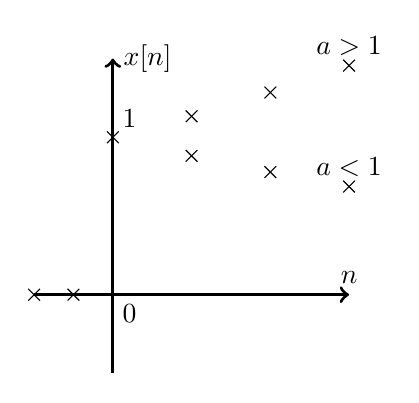
\begin{tikzpicture}[scale=2]
        \draw[->,very thick](-0.5,0)--(1.5,0)node[above]{$n$};
        \draw[->,very thick](0,-0.5)--(0,1.5)node[right]{$x[n]$};

        \draw(-0.5,0)pic[black]{cross=3pt};
        \draw(-0.25,0)pic[black]{cross=3pt};
        \draw(0,1)pic[black]{cross=3pt};

        \draw(0.5,1.133)pic[black]{cross=3pt};
        \draw(0.5,0.882)pic[black]{cross=3pt};
        \draw(1,1.284)pic[black]{cross=3pt};
        \draw(1,0.779)pic[black]{cross=3pt};
        \draw(1.5,1.455)pic[black]{cross=3pt};
        \draw(1.5,0.687)pic[black]{cross=3pt};

        \node[above]at(1.5,1.455){$a>1$};
        \node[above]at(1.5,0.687){$a<1$};

        \node[above right]at(0,1){$1$};
        \node[below right]at(0,0){$0$};
    \end{tikzpicture}
\end{center}

\subsection{Coseno}

\begin{equation*}
    x[n]=\cos(2\pi f_0n)
\end{equation*}

Il segnale è periodico nel discreto, solo se la frequenza è un numero intero $f_0\in\mathbb{Z}$. 

\begin{center}
    \begin{tikzpicture}[scale=2]
        \draw[->,very thick](0,-1.5)--(0,1.5)node[right]{$x[n]$};
        \draw[->,very thick](-2,0)--(2,0)node[right]{$n$};   
     
        \draw (0,1)pic[black]{cross=3pt};
        \draw (0.5,-1)pic[black]{cross=3pt};
        \draw (-0.5,-1)pic[black]{cross=3pt};
        \draw (1,1)pic[black]{cross=3pt};
        \draw (-1,1)pic[black]{cross=3pt};
        \draw (1.5,-1)pic[black]{cross=3pt};
        \draw (-1.5,-1)pic[black]{cross=3pt};
        \draw (2,1)pic[black]{cross=3pt};
        \draw (-2,1)pic[black]{cross=3pt};


        \node[above right]at(0,1){$1$};
        \node[below left]at(0,-1){$-1$};
        \node[below right]at(0,0){$0$};
    \end{tikzpicture}
\end{center}

\subsection{Impulso Matematico Tempo Discreto}

L'impulso matematico o delta di Dirac, nel discreto assume solo un valore di $1$ per $n=0$. 
\begin{equation*}
    \delta[n]:=\begin{cases}
        1&n=0\\
        0&n\neq0
    \end{cases}
\end{equation*}

Questo segnale presenta varie proprietà utili:


L'area della delta è unitaria, poiché presenta un unico campione per $n=0$ di valore $1$:
\begin{equation*}
    \displaystyle\sum_{n=-\infty}^{+\infty}\delta[n]=1
\end{equation*}



Il prodotto di un qualsiasi segnale $x[n]$ per la delta equivale al valore del segnale in $0$ per la delta. Poiché l'unico valore della delta diverso da zero si trova in $n=0$ 
e vale $1$, per cui estra dal segnale $x$ il campione in posizione $n=0$. Questo campione viene moltiplicato per la delta, poiché non è un segnale continuo, ma si presenta 
solo in quell'istante. Questa caratteristica viene chiamata propietà di campionamento 
della delta di Dirac:
\begin{equation*}
    x[n]\cdot\delta[n]=x[0]\cdot\delta[n]
\end{equation*}
Questo campione può essere estratto ad un arbitrario valore $m$:
\begin{equation*}
    x[n]\cdot\delta[n-m]=x[m]\cdot\delta[n-m]
\end{equation*}


L'area del prodotto di un qualsiasi segnale $x[n]$ per la delta risulta nel valore del segnale in $0$, ciò si dimostra tramite la proprietà di campionamento della delta:
\begin{equation*}
    \displaystyle\sum_{n=-\infty}^{+\infty} x[n]\cdot\delta[n]=\sum_{n=-\infty}^{+\infty} x[0]\cdot\delta[n]=x[0]\cancelto{1}{\sum_{n=-\infty}^{+\infty}\delta[n]}=x[0]
\end{equation*}


Invertendo la proprietà di campionamendo, ovvero partendo da tutti i campioni di un segnale $x[n]$ e sommandoli tra di loro, è possibile ottenere il segnale originario: 
\begin{equation*}
    \cdots+x[-N]\delta[n+N]+\cdots+x[0]\delta[n]+\cdots+x[N]\delta[n-N]+\cdots=\displaystyle\sum_{i=-\infty}^{+\infty} x[i]\delta[n-i]=x[n]
\end{equation*}


La convoluzione di un qualsiasi segnale $x[n]$ per la delta risulta nel segnale $x$ stesso:
\begin{equation*}
    x[n]*\delta[n]=\displaystyle\sum_{k=-\infty}^{+\infty}x[k]\delta[n-k]=\sum_{k=-\infty}^{+\infty}x[n]\delta[n-k]=x[n]\cancelto{1}{\sum_{k=-\infty}^{+\infty}\delta[n-k]}
\end{equation*}


La delta può essere rappresentata come la differenza tra due gradini, considerando un unico campione in posizione $m$:
\begin{equation*}
    \delta[n-m]=u[n-m]-u[n-(m+1)]
\end{equation*}



Analogamente un gradino può essere espresso come una sommatoria di delta traslate ognuna di un diverso fattore. Questa relazione viene espressa in forma canonica come:
\begin{equation*}
    u[n-m]=\displaystyle\sum_{n=-\infty}^{-m}\delta[n+1]
\end{equation*}

\subsection{Energia e Potenza}

L'energia di un segnale tempo discreto si calcola come:
\begin{equation*}
    E_x:=\displaystyle\lim_{N\to\infty}\sum_{n=-N}^N|x[n]|^2
\end{equation*}
La potenza di un segnale tempo discreto è defintia come:
\begin{equation*}
    P_x:=\displaystyle\lim_{N\to\infty}\left(\frac{1}{2N+1}\sum_{n=-N}^N|x[n]|^2\right)
\end{equation*}
La potenza per segnali periodici tempo discreti si ottiene mediante:
\begin{equation*}
    P_x:=\displaystyle\frac{1}{M}\sum_{n=0}^{M-1}|x[n]|^2
\end{equation*}
Dove $M$ è il periodo del segnale

\clearpage

\section{Convoluzione e Correlazione}

Prima di analizzare queste due importanti operazioni tra segnali tempo continuo e discreto, bisogna fornire una definizione adeguata per l'impulso matematico tempo 
continuo, segnale necessario per poter analizzare facilmente le proprietà di queste operazioni. 

\subsection{Impulso Matematico Tempo Continuo}

Per definire l'impulso o delta di Dirac nel tempo continuo, si parte da un segnale finestra con una base $\Delta t$ e ampiezza inverso della base:
\begin{equation*}
    x(t)=\displaystyle\frac{1}{\Delta t}\mbox{rect}\left(\frac{t}{\Delta t}\right)
\end{equation*}

\begin{center}
    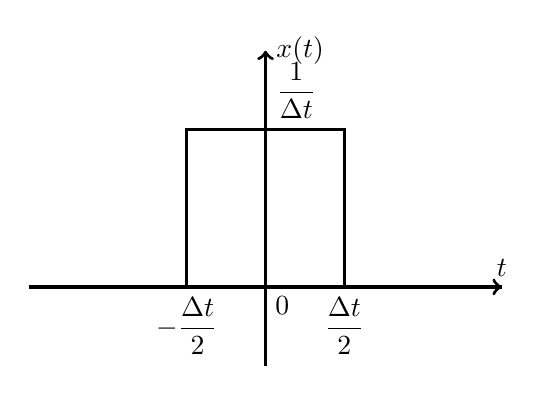
\begin{tikzpicture}[scale=2]
        \draw[->,very thick](-1.5,0)--(1.5,0)node[above]{$t$};
        \draw[->,very thick](0,-0.5)--(0,1.5)node[right]{$x(t)$};
        \node[below right]at(0,0){$0$};

        \draw[-,very thick](-1.5,0)--(-0.5,0)node[below]{$\displaystyle-\frac{\Delta t}{2}$}--(-0.5,1)--(0,1)node[above right]{$\displaystyle\frac{1}{\Delta t}$}--(0.5,1)--(0.5,0)node[below]{$\displaystyle\frac{\Delta t}{2}$}--(1.5,0);        
    \end{tikzpicture}
\end{center}

Al diminuire di $\Delta t$, la base si restringe, mentre l'ampiezza del segnale aumenta, ma complessivamente l'area del segnale rimane unitaria:
\begin{equation*}
    \displaystyle\int_{-\infty}^{+\infty}x(t)dt=\frac{1}{\Delta t}\int_{-\frac{\Delta t}{2}}^{\frac{\Delta t}{2}}dt=\frac{1}{\Delta t}\left(\frac{\Delta t}{2}+\frac{\Delta t}{2}\right)=1
\end{equation*}

Viene definito l'impulso o dela di Dirac come il limite di questa finestra per $\Delta t$ che tende ad un valore infinito:
\begin{equation*}
    \delta(t):=\lim_{\Delta t\to\infty}\displaystyle\frac{1}{\Delta t}\mbox{rect}\left(\frac{t}{\Delta t}\right)
\end{equation*}

Viene rappresentata graficamente come una freccia di altezza unitaria, poiché non è una funzione ma un funzionale. Si tratta in telecomunicazioni come un segnale qualuneque. 
\begin{center}
    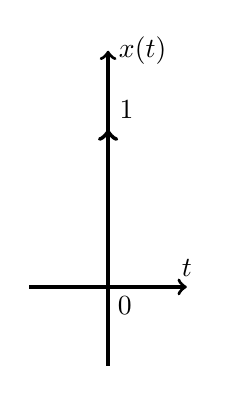
\begin{tikzpicture}[scale=2]
        \draw[->,very thick](-0.5,0)--(0.5,0)node[above]{$t$};
        \draw[->,very thick](0,-0.5)--(0,1.5)node[right]{$x(t)$};
        \node[below right]at(0,0){$0$};

        \draw[->,ultra thick](0,0)--(0,1)node[above right]{$1$};
    \end{tikzpicture}
\end{center}

Possiede delle proprietà analoghe alla delta nel tempo discreto:



L'integrale sui reali della delta è unitario in base alla sua definizione:
\begin{equation*}
    \displaystyle\int_{-\infty}^{+\infty}\delta(t)dt=1
\end{equation*}



Il prodotto di un qualsiasi segnale per la delta equivale al valore del segnale in $0$ moltiplicato per l'impulso, poiché per tutti gli altri valori nel tempo questo prodotto 
è nullo. Proprietà analoga a quella del campionamento per il continuo:
\begin{equation*}
    x(t)\cdot\delta(t)=x(0)\cdot\delta(t)
\end{equation*}
Questa proprietà può essere estesa considerando un impulso traslato di un fattore $\tau$:
\begin{equation*}
    x(t)\cdot\delta(t-\tau)=x(\tau)\cdot\delta(t-\tau)
\end{equation*}



Segue da quest'ultima che l'integrale del prodotto di un segnale qualunque $x(t)$ per l'impulso equivale al valore del segnale $x$ in $0$:
\begin{equation*}
    \displaystyle\int_{-\infty}^{+\infty}x(t)\cdot\delta(t)dt=\int_{-\infty}^{+\infty}x(0)\cdot\delta(t)dt=x(0)\cancelto{1}{\int_{-\infty}^{+\infty}\delta(t)dt}=x(0)
\end{equation*}



La convoluzione di un qualsiasi segnale $x(t)$ con l'impulso risulta nel segnale originario $x(t)$, per l'inverso della proprietà precedente: 
\begin{equation*}
    x(t)*\delta(t)=\displaystyle\int_{-\infty}^{+\infty}x(\tau)\cdot\delta(t-\tau)d\tau=x(t)\cancelto{1}{\int_{-\infty}^{+\infty}\delta(t-\tau)d\tau}=x(t)
\end{equation*}



Poiché il segnale finestra può essere espresso come la differenza tra due gradini, allora anche la definizione dell'impulso può essere espressa come tale:
\begin{equation*}
    \delta(t):=\lim_{\Delta t\to\infty}\frac{1}{\Delta t}\left(u\left(t+\frac{\Delta t}{2}\right)-u\left(t-\frac{\Delta t}{2}\right)\right)
\end{equation*}



L'impulso corrisponde alla derivata rispetto al tempo del gradino. Analogamente il gradino corrisponde alla funzione integrale dell'impulso:
\begin{gather*}
    \delta(t)=\displaystyle\frac{du(t)}{dt}\\
    u(t)=\displaystyle\int_{-\infty}^t\delta(\tau)d\tau
\end{gather*}



L'impulso è una funzione pari:
\begin{equation*}
    \delta(t)=\delta(-t)
\end{equation*}



L'impulso scalato di un fattore $a$ corrisponde all'impulso non scalato fratto il modulo del fattore $a$, se negativo. Questa proprietà di scala si dimostra considerando 
la definizione dell'impulso. 
\begin{equation*}
    \delta(at)=\displaystyle\frac{\delta(t)}{a}
\end{equation*}



L'impulso è un segnale né di energia né di potenza. I funzionali, come l'impulso, vengono descritti in base agli effetti che provocano sulle funzioni

\subsection{Convoluzione}

La convoluzione rappresenta un'operazione tra due segnali, generandone uno nuovo. L'operazione si indica con il simbolo $*$:
\begin{equation*}
    x(t)*y(t)=z(t)
\end{equation*}

La convoluzione tra due segnali tempo continui produce un altro segnlae tempo continuo. La convoluzione risultante è sempre un segnale continuo:
\begin{equation}
    z(t)=x(t)*y(t):=\displaystyle\int_{-\infty}^{+\infty}x(\tau)\cdot y(t-\tau)d\tau
\end{equation}

Il segnale convoluzione è una funzione nella stessa variabile dei segnali convoluti, questa variabile di uscita compare all'interno dell'integrale. Il segnale conoluzione 
rappresenta l'area sottesa dal prodotto tra il segnale $x$ ed il segnale $y$, ribaltato e traslato di un fattore $t$, per ogni istante di tempo $t$. La convoluzione 
è un'operazione commutativa, per cui è arbitraria la scelta di quale dei due segnali debba traslare. 

Si rappresenta il segnale $x$ originiario rispetto alla variabile $\tau$, al di sotto si grafica il segnale $y$ ribaltato e traslato di un fattore $t$, per individuare gli 
intervalli dove il prodotto tra i due segnali è nullo. La maggior parte dei segnali reali si attenuano nel tempo, per cui avranno un valore solo per un intervallo finito 
di valori, ed in questi intervalli la convoluzione restituisce un valore non nullo. Anche nei segnali puramente matematici, spesso presentano valori finiti non nulli solo per 
certi intervalli di tempo. Si considerano tutti i possibili casi di sovrapposizione, quindi di prodotto non nullo, tra i due segnali per ottenere 
il segnale convoluzione in forma analitica, da ricordare che la convoluzione è un segnale continuo per cui non possono essere presenti discontinuità nella sua espressione 
in forma anlitica. 



Vengono forniti alcuni esempi di convoluzioni:

\subsubsection{Esponenziale Unilatero per Gradino}

Si considera $\alpha\in\mathbb{R}^+$. 
\begin{equation*}
    z(t)=e^{-\alpha t}u(t)*u(t)=\displaystyle\int_{-\infty}^{+\infty}e^{-\alpha\tau}u(\tau)u(t-\tau)d\tau
\end{equation*}
Poiché è presente un gradino nell'integrale, la convoluzione assumerà valori nulli per $t<0$, ciò si può anche individure graficamente, poiché per gli stessi valori i due 
graficie del gradino e delò'esponenziale unilatero non si sovrappongono. All'aumentare del valore di $t$, il valore del segnale $z(t)$ aumenta sempre più lentamente, poiché i 
contributi dell'esponenziale vanno diminuendo. Poiché entrambi i gradini nell'integrale assumono valori unitari per $t>0$, il valore del segnale in questo intervallo 
dipende dalla funzione integrale dell'esponenziale, da $0$ al valore di $t$ corrente:
\begin{equation*}
    z(t)=\begin{cases}
        0&t<0\\
        \displaystyle\int_0^te^{-\alpha \tau}d\tau&t\geq0
    \end{cases}
\end{equation*}
Risolvendo l'integrale si ottiene:
\begin{equation*}
    \displaystyle\int_0^te^{-\alpha \tau}d\tau=\left|-\frac{e^{-\alpha\tau}}{\alpha}\right|^t_0=\frac{1-e^{-\alpha t}}{\alpha}
\end{equation*}
Per cui il segnale convoluzione in forma analitica risulta:
\begin{equation*}
    z(t)=\begin{cases}
        0&t<0\\
        \displaystyle\frac{1-e^{-\alpha t}}{\alpha}&t\geq0
    \end{cases}
\end{equation*}
Questo segnale tende asintoticamente a $1/\alpha$ per $t\to+\infty$. 

\begin{center}
    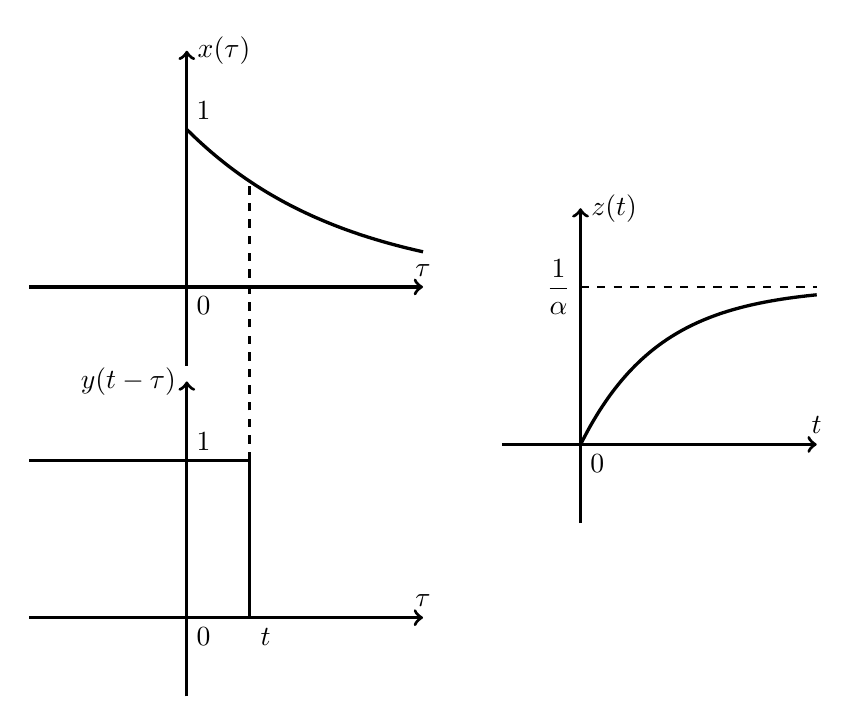
\begin{tikzpicture}[scale=2]
        \draw[->,very thick](-1,0)--(1.5,0)node[above]{$\tau$};
        \draw[->,very thick](0,-0.5)--(0,1.5)node[right]{$x(\tau)$};
        \node[below right]at(0,0){$0$};
        \node[above right]at(0,1){$1$};

        \draw[-,very thick]plot[smooth, domain=0:1.5](\x,{e^(-\x)});

        \draw[->,very thick](-1,-2.1)--(1.5,-2.1)node[above]{$\tau$};
        \draw[->,very thick](0,-2.6)--(0,-0.6)node[left]{$y(t-\tau)$};
        \node[below right]at(0,-2.1){$0$};
        \node[above right]at(0,-1.1){$1$};

        \draw[-,very thick](-1,-1.1)--(0.4,-1.1)--(0.4,-2.1)node[below right]{$t$};
        \draw[dashed,very thick](0.4,-1.1)--(0.4,0.67);


        \draw[->,very thick](2,-1)--(4,-1)node[above]{$t$};
        \draw[->,very thick](2.5,-1.5)--(2.5,0.5)node[right]{$z(t)$};
        \node[below right]at(2.5,-1){$0$};
        \node[left]at(2.5,0){$\displaystyle\frac{1}{\alpha}$};
        \draw[dashed](2.5,0)--(4,0);
        \draw[-,very thick]plot[smooth, domain=2.5:4](\x,{-e^(-2*(\x-2.5))});
    \end{tikzpicture}
\end{center}

\subsubsection{Autoconvoluzione di Un Esponenziale Unilatero}

\begin{equation*}
    z(t)=e^{-\alpha t}u(t)*e^{-\alpha t}u(t)=\displaystyle\int_{-\infty}^{+\infty}e^{-\alpha\tau}u(\tau)e^{-\alpha(t-\tau)}u(t-\tau)d\tau
\end{equation*}
Poiché sono unilateri, non si sovrapporrano per $t<0$, quindi la convoluzione è nulla per quei valori di tempo. Può essere spiegato tramite la prorpietà del gradino di 
cambiare i limiti di integrazione, per cui invece di integrare da $-\infty$ a $+\infty$, si integra nell'intervallo dove si trova il gradino $u(\tau)$, ovvero da $0$ a $+\infty$: 
\begin{equation*}
    z(t)=\displaystyle\int_0^{+\infty}e^{-\alpha t}u(t-\tau)d\tau=e^{-\alpha t}\int_0^{+\infty}u(t-\tau)d\tau
\end{equation*}
L'area sottesa da un gradino ribaltato e traslato di un fattore $t>0$ da $0$ a $+\infty$ equivale all'area di un rettangolo di altezza $1$ e di base $t$:
\begin{equation*}
    z(t)=e^{-\alpha t}\displaystyle\int_0^td\tau=te^{-\alpha t}
\end{equation*}

In forma analitica risulta:
\begin{equation*}
    z(t)=\begin{cases}
        0&t<0\\
        te^{-\alpha t}&t\geq0
    \end{cases}
\end{equation*}
 

\begin{center}
    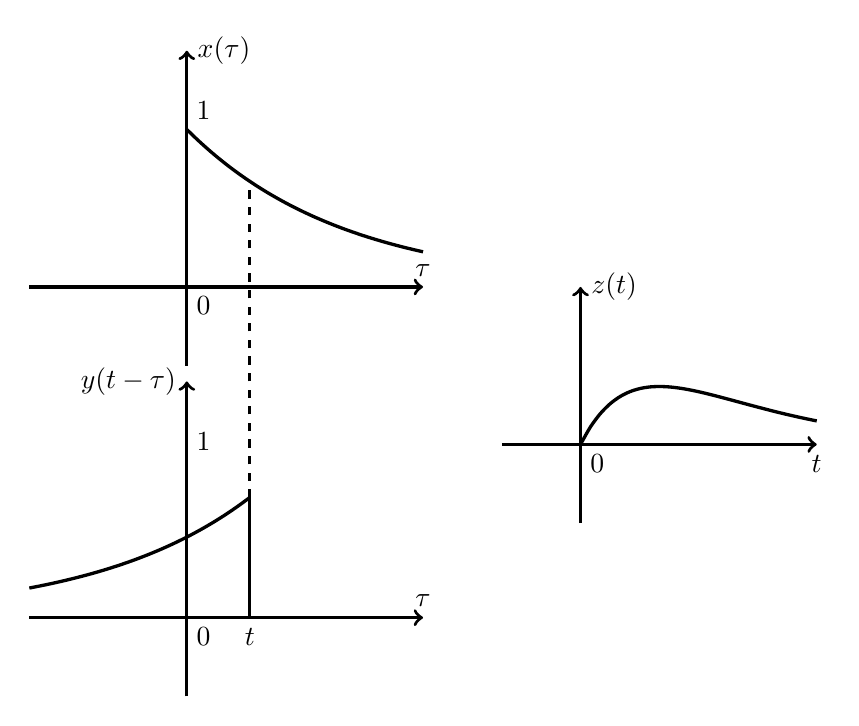
\begin{tikzpicture}[scale=2]
        \draw[->,very thick](-1,0)--(1.5,0)node[above]{$\tau$};
        \draw[->,very thick](0,-0.5)--(0,1.5)node[right]{$x(\tau)$};
        \node[below right]at(0,0){$0$};
        \node[above right]at(0,1){$1$};

        \draw[-,very thick]plot[smooth, domain=0:1.5](\x,{e^(-\x)});

        \draw[->,very thick](-1,-2.1)--(1.5,-2.1)node[above]{$\tau$};
        \draw[->,very thick](0,-2.6)--(0,-0.6)node[left]{$y(t-\tau)$};
        \node[below right]at(0,-2.1){$0$};
        \node[above right]at(0,-1.1){$1$};

        \draw[-,very thick]plot[smooth, domain=-1:0.4](\x,{e^(\x-0.67)-2.1});
        \draw[-,very thick](0.4,-2.1)node[below]{$t$}--(0.4,-1.337);
        \draw[dashed,very thick](0.4,-1.337)--(0.4,0.67);


        \draw[->,very thick](2,-1)--(4,-1)node[below]{$t$};
        \draw[->,very thick](2.5,-1.5)--(2.5,0)node[right]{$z(t)$};
        \node[below right]at(2.5,-1){$0$};
        \draw[-,very thick]plot[smooth, domain=2.5:4](\x,{2*(\x-2.5)*e^(-2*(\x-2.5))-1});
    \end{tikzpicture}
\end{center}

\subsubsection{Convoluzione tra Due Finestre}

Si considerano due casi, dove le due finestra hanno base uguale, ed un caso dove hanno base differente. Si considera il caso $T_1=T_2$:
\begin{equation*}
    z(t)=\mbox{rect}\left(\displaystyle\frac{t}{T}\right)*\mbox{rect}\left(\frac{t}{T}\right)
\end{equation*}

La convoluzione assume valori nulli quando non si sovrappongono, ovvero per un valore $t+\displaystyle\frac{T}{2}<-\frac{T}{2}\to t<-T$. L'area sottesa dal prodotto 
di queste due finestre aumenta linearmente fino a quando non si sovrappongono per $t=0$, dove l'area assume valore massimo $T\cdot 1$, dopo il quale 
decresce linearmente fino a $t=T$. Se una delle due fosse stata traslata di un fattore $t_0$, l'intera convoluzione sarebbe stata traslata dello stesso fattore. Da notare 
che la convoluzione di due segnali pari genera un segnale pari.  
\begin{equation*}
    z(t)=\begin{cases}
        0&t<-T\\
        \displaystyle\int_{-T}^td\tau&-T\leq t<0\\
        \displaystyle\int_t^Td\tau&0\leq t<T\\
        0&t>T
    \end{cases}=\begin{cases}
        0&t<-T\land t>T\\
        T-|t|&-T\leq t<T\\
    \end{cases}=T\,\mbox{tri}\left(\displaystyle\frac{t}{T}\right)
\end{equation*}
La convoluzione tra due finestre di base uguale risulta in un triangolo di base doppia $2T$, e scalata di un fattore pari alla base $T$. 

\begin{center}
    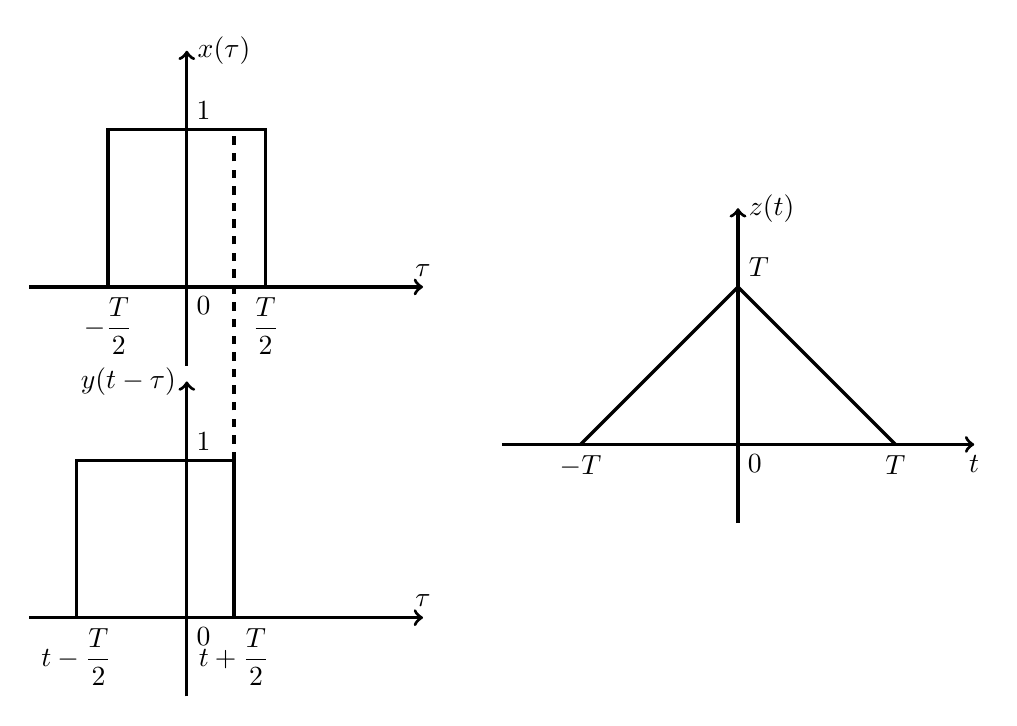
\begin{tikzpicture}[scale=2]
        \draw[->,very thick](-1,0)--(1.5,0)node[above]{$\tau$};
        \draw[->,very thick](0,-0.5)--(0,1.5)node[right]{$x(\tau)$};
        \node[below right]at(0,0){$0$};
        \node[above right]at(0,1){$1$};

        \draw[-,very thick](-0.5,0)node[below]{$-\displaystyle\frac{T}{2}$}--(-0.5,1)--(0.5,1)--(0.5,0)node[below]{$\displaystyle\frac{T}{2}$};

        \draw[->,very thick](-1,-2.1)--(1.5,-2.1)node[above]{$\tau$};
        \draw[->,very thick](0,-2.6)--(0,-0.6)node[left]{$y(t-\tau)$};
        \node[below right]at(0,-2.1){$0$};
        \node[above right]at(0,-1.1){$1$};

        \draw[-,very thick](0.3,-2.1)node[below]{$t+\displaystyle\frac{T}{2}$}--(0.3,-1.1)--(-0.7,-1.1)--(-0.7,-2.1)node[below]{$t-\displaystyle\frac{T}{2}$};
        \draw[dashed,very thick](0.3,-1.1)--(0.3,1);


        \draw[->,very thick](2,-1)--(5,-1)node[below]{$t$};
        \draw[->,very thick](3.5,-1.5)--(3.5,0.5)node[right]{$z(t)$};
        \node[below right]at(3.5,-1){$0$};
        \draw[-,very thick](2.5,-1)node[below]{$-T$}--(3.5,0)node[above right]{$T$}--(4.5,-1)node[below]{$T$};
    \end{tikzpicture}
\end{center}

Si considera ora il caso dove le due finestre hanno basi $T_1>T_2$:
\begin{equation*}
    z(t)=\mbox{rect}\left(\displaystyle\frac{t}{T_1}\right)*\mbox{rect}\left(\frac{t}{T_2}\right)
\end{equation*}

Poiché le due finestre sono simmetriche, si analizzano solo i casi per $t<0$, per poi aggiungere per simmetria l'equazione analitica per $t\geq0$. Le due finestre non si 
sovrappongono per $t+\displaystyle\frac{T_2}{2}<-\frac{T_1}{2}\to t<-\frac{1}{2}(T_1+T_2)$, per cui in quell'intervallo la convoluzione assume valore nullo. Il valore 
della convoluzione aumenta linearmente fino a quando la finestra più piccola trasla fino ad essere completamente interna alla finestra di base $T_1$ per un valore 
$t-\displaystyle\frac{T_2}{2}<-\frac{T_1}{2}\to t<-\frac{1}{2}(T_1-T_2)$. Quando le due finestre si sovrappongono, il valore della convoluzione è costante, e corrisponde 
all'area di un rettangolo di base, base della finestra più piccola $T_2$ ed altezza unitaria $T_2\cdot1$ fino a raggiungere $t_0$. Ribaltando questo segnale ottenuto 
si ottiene il segnale per valori $t\geq0$:
\begin{gather*}
    z(t)=\begin{cases}
        0&t<-\displaystyle\frac{1}{2}(T_1+T_2)\\
        \displaystyle\int_{-\frac{1}{2}(T_1+T_2)}^td\tau&-\frac{1}{2}(T_1+T_2)\leq t <-\frac{1}{2}(T_1-T_2)\\
        T_2&-\frac{1}{2}(T_1-T_2)\leq t<\frac{1}{2}(T_1-T_2)\\
        -\displaystyle\int_{-\frac{1}{2}(T_1+T_2)}^td\tau&\frac{1}{2}(T_1-T_2)\leq t <\frac{1}{2}(T_1+T_2)\\
        0&t\geq\displaystyle\frac{1}{2}(T_1+T_2)
    \end{cases}\\
    z(t)=\begin{cases}
        0&t<-\displaystyle\frac{1}{2}(T_1+T_2)\land t\geq\frac{1}{2}(T_1+T_2)\\
        \displaystyle\frac{1}{2}(T_1+T_2)-|t| &-\frac{1}{2}(T_1+T_2)\leq t <-\frac{1}{2}(T_1-T_2)\land \frac{1}{2}(T_1-T_2)\leq t <\frac{1}{2}(T_1+T_2)\\
        T_2&-\displaystyle\frac{1}{2}(T_1-T_2)\leq t<\frac{1}{2}(T_1-T_2)
    \end{cases}
\end{gather*}

\begin{center}
    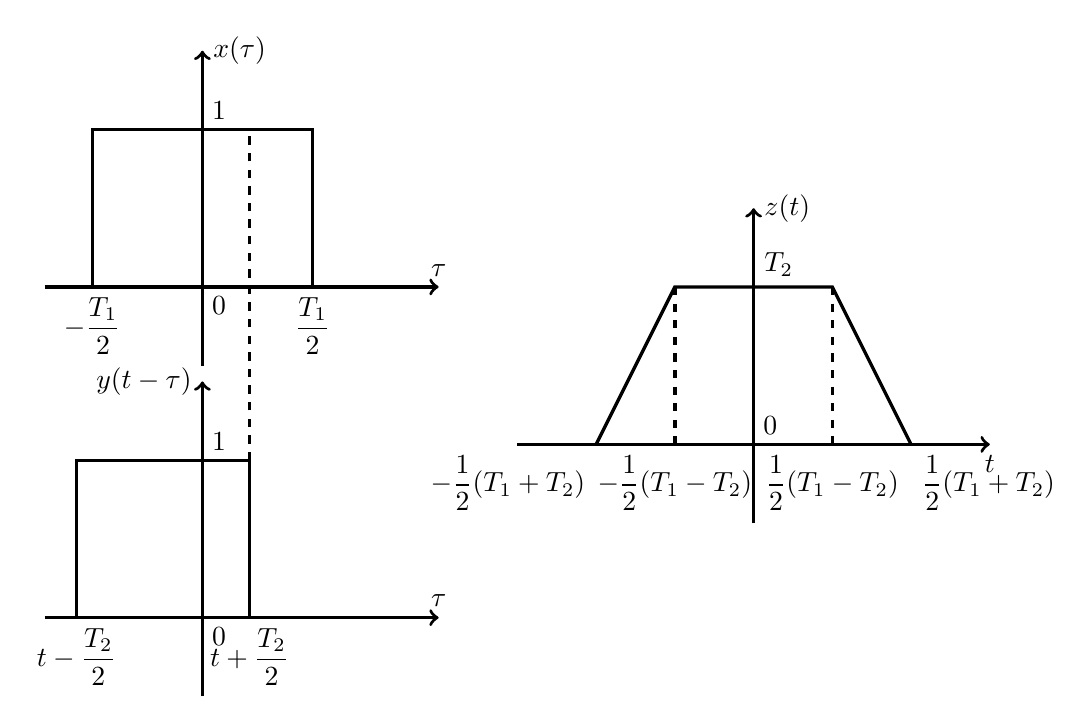
\begin{tikzpicture}[scale=2]
        \draw[->,very thick](-1,0)--(1.5,0)node[above]{$\tau$};
        \draw[->,very thick](0,-0.5)--(0,1.5)node[right]{$x(\tau)$};
        \node[below right]at(0,0){$0$};
        \node[above right]at(0,1){$1$};

        \draw[-,very thick](-0.7,0)node[below]{$-\displaystyle\frac{T_1}{2}$}--(-0.7,1)--(0.7,1)--(0.7,0)node[below]{$\displaystyle\frac{T_1}{2}$};

        \draw[->,very thick](-1,-2.1)--(1.5,-2.1)node[above]{$\tau$};
        \draw[->,very thick](0,-2.6)--(0,-0.6)node[left]{$y(t-\tau)$};
        \node[below right]at(0,-2.1){$0$};
        \node[above right]at(0,-1.1){$1$};

        \draw[-,very thick](0.3,-2.1)node[below]{$t+\displaystyle\frac{T_2}{2}$}--(0.3,-1.1)--(-0.8,-1.1)--(-0.8,-2.1)node[below]{$t-\displaystyle\frac{T_2}{2}$};
        \draw[dashed,very thick](0.3,-1.1)--(0.3,1);


        \draw[->,very thick](2,-1)--(5,-1)node[below]{$t$};
        \draw[->,very thick](3.5,-1.5)--(3.5,0.5)node[right]{$z(t)$};
        \node[above right]at(3.5,-1){$0$};
        \draw[-,very thick](2.5,-1)node[below left]{$-\displaystyle\frac{1}{2}(T_1+T_2)$}--(3,0)--(3.5,0)node[above right]{$T_2$}--(4,0)--(4.5,-1)node[below right]{$\displaystyle\frac{1}{2}(T_1+T_2)$};
        \draw[dashed, very thick](3,0)--(3,-1)node[below]{$\displaystyle-\frac{1}{2}(T_1-T_2)$};
        \draw[dashed, very thick](4,0)--(4,-1)node[below]{$\displaystyle\frac{1}{2}(T_1-T_2)$};
    \end{tikzpicture}
\end{center}

Il grafico di questa convoluzione rappresenta un trapezio di altezza $T_2$, base maggiore $T_1+T_2$ e base minore $T_1-T_2$ Si nota come l'autoconvoluzione di due finestre 
di base uguali rappresenta un caso speciale di questo trapezio, avente base minore nulla $T-T=0$ e base doppia rispetto alla finestra $T+T=2T$, ciò equivale ad un triangolo 
di altezza $T$ e base $2T$. 

\subsubsection{Convoluzione tra Due Gaussiane}

Date due gaussiane definite dai parametri $\alpha_1$ e $\alpha_2$, con $\alpha_1,\alpha_2\in\mathbb{R}^+$, si vuole determinare la convoluzione tra questi due segnali:
\begin{gather*}
    z(t)=e^{-\alpha_1t^2}*e^{-\alpha_2t^2}=\displaystyle\int_{-\infty}^{+\infty}e^{-\alpha_1\tau^2}e^{-\alpha_2(t-\tau)^2}d\tau=\int_{-\infty}^{+\infty}e^{-\alpha_1\tau^2}e^{-\alpha_2(t^2-2t\tau+\tau^2)}d\tau\\
    \displaystyle e^{-\alpha_2 t^2}\int_{-\infty}^{+\infty}e^{-(\alpha_1+\alpha_2)\tau^2}e^{2\alpha_2t\tau^2}d\tau=e^{-\alpha_2 t^2}\int_{-\infty}^{+\infty}e^{-(\alpha_1+\alpha_2)\left[\tau^2-2\alpha_2\frac{t\tau}{\alpha_1+\alpha_2}\right]}d\tau
\end{gather*}

Si somma e si sottrae il fattore $\displaystyle\left(\frac{\alpha_2t}{\alpha_1+\alpha_2}\right)^2$ nell'esponenziale all'interno dell'integrale:
\begin{gather*}
    \displaystyle e^{-\alpha_2 t^2}\int_{-\infty}^{+\infty}e^{-(\alpha_1+\alpha_2)\left[\tau^2-2\alpha_2\frac{t\tau}{\alpha_1+\alpha_2}+\left(\frac{\alpha_2t}{\alpha_1+\alpha_2}\right)^2-\left(\frac{\alpha_2t}{\alpha_1+\alpha_2}\right)^2\right]}d\tau\\
    \displaystyle e^{-\alpha_2 t^2}\int_{-\infty}^{+\infty}e^{-(\alpha_1+\alpha_2)\left[\left(\tau-\frac{\alpha_2t}{\alpha_1+\alpha_2}\right)^2-\left(\frac{\alpha_2t}{\alpha_1+\alpha_2}\right)^2\right]}d\tau\\
    \displaystyle e^{-\left(\alpha_2-\frac{\alpha_2^2}{\alpha_1+\alpha_2}\right)t^2}\int_{-\infty}^{+\infty}e^{-(\alpha_1+\alpha_2)\left[\tau-\frac{\alpha_2t}{\alpha_1+\alpha_2}\right]^2}d\tau
\end{gather*}
Si applica la sostituzione $T=\displaystyle\sqrt{\alpha_1+\alpha_2}\left(\tau+\frac{\alpha_2t}{\alpha_1+\alpha_2}\right)$:
\begin{equation*}
    \displaystyle e^{-\left(\frac{\alpha_1\alpha_2}{\alpha_1+\alpha_2}\right)t^2}\int_{-\infty}^{+\infty}\frac{e^{-T^2}}{\sqrt{\alpha_1+\alpha_2}}dT=\frac{e^{-\left(\frac{\alpha_1\alpha_2}{\alpha_1+\alpha_2}\right)t^2}}{\sqrt{\alpha_1+\alpha_2}}\int_{-\infty}^{+\infty}{e^{-T^2}}dT
\end{equation*}
Il fattore integrale corrisponde all'integrale di Gauss, precedentemente discusso, che risulta su tutti i reali in un area di $\sqrt\pi$:
\begin{equation*}
    e^{-\alpha_1t^2}*e^{-\alpha_2t^2}=\displaystyle\sqrt{\frac{\pi}{\alpha_1+\alpha_2}}e^{-\frac{\alpha_1\alpha_2}{\alpha_1+\alpha_2}t^2}
\end{equation*}
Esprimendo le due gaussiane in forma normalizzata, risulta che la varianza della convoluzione equivale alla somma delle varianze delle due gaussiane $\sigma=\sigma_1+\sigma_2$:
\begin{equation}
    \displaystyle\frac{1}{\sqrt{2\pi}\sigma_1}e^{-\frac{t^2}{2\sigma_1}}*\frac{1}{\sqrt{2\pi}\sigma_2}e^{-\frac{t^2}{2\sigma_2}}=\frac{1}{\sqrt{2\pi(\sigma_1^2+\sigma_2^2)}}e^{-\frac{t^2}{2(\sigma_1^2+\sigma_2^2)}}
\end{equation}

\subsubsection{Proprietà}

La convoluzione è un'operazione commutativa:
\begin{equation*}
    x(t)*y(t)=\displaystyle\int_{-\infty}^{+\infty}x(\tau)y(t-\tau)d\tau \to^{T=t-\tau}\to \int_{-\infty}^{+\infty}y(T)x(t-T)dT=y(t)*x(t)
\end{equation*}
Vale la proprietà distributiva:
\begin{gather*}
    (x_1(t)+x_2(t))*y(t)=\displaystyle\int_{-\infty}^{+\infty}(x_1(\tau)+x_2(\tau))y(t-\tau)d\tau\\
    \int_{-\infty}^{+\infty}x_1(\tau)y(t-\tau)d\tau+\int_{-\infty}^{+\infty}x_2(\tau)y(t-\tau)d\tau=x_1(t)*y(t)+x_2(t)*y(t)
\end{gather*}

Se una dei due segnali, o entrambi, convoluti tra di loro sono traslati allora il segnale convoluzione risultante è traslato della traslazione complessiva dei due segnali originali:
\begin{gather*}
    x(t-t_{x0})*y(t-t_{y0})=\displaystyle\int_{-\infty}^{+\infty}x(\tau-t_{x0})y(t-(\tau+t_{y0}))d\tau,\,{T=\tau-t_{x0}}\to\\
    \int_{-\infty}^{+\infty}x(T)y((t-t_{x0}-t_{y0})+T)dT=z(t-t_{x0}-t_{y0})
\end{gather*}

\subsubsection{Convoluzione di Una Finestra per Segnale Periodico}


Per semplificare i calcoli, si considera il segnale coseno, ma le proprietà ottenuta da quest'operazione valgono per ogni funzione periodica, non attenuata nel tempo. 

\begin{equation*}
    z(t)=\mbox{rect}\displaystyle\left(\frac{t}{T_1}\right)*\cos\left(\frac{2\pi t}{T_2}\right)=\int_{-\infty}^{+\infty}\cos\left(\frac{2\pi \tau}{T_2}\right)\mbox{rect}\displaystyle\left(\frac{t-\tau}{T_1}\right)d\tau
\end{equation*}
La funzione è periodica per cui non è necessario valutare quando la convoluzione è nulla. Il prodotto tra i due segnali è non nullo per valori di $\tau$ compresi tra 
$\displaystyle\frac{T_1}{2}-t$ e $-\displaystyle\frac{T_1}{2}-t$:
\begin{gather*}
    z(t)=\displaystyle\int_{-\frac{T_1}{2}-t}^{\frac{T_1}{2}-t}\cos\left(\frac{2\pi\tau}{T_2}\right)d\tau=\frac{T_2}{2\pi}\sin\left(\frac{2\pi\tau}{T_2}\right)\Bigg|_{-\frac{T_1}{2}-t}^{\frac{T_1}{2}-t}\\
    \displaystyle\frac{T_2}{2\pi}\left[\sin\left(\frac{2\pi(t+\frac{T_1}{2})}{T_2}\right)-\sin\left(\frac{2\pi(t-\frac{T_1}{2})}{T_2}\right)\right]
\end{gather*}
Per la seconda formula di prostaferesi si ottiene:
\begin{gather*}
    z(t)=\displaystyle\frac{T_2}{2\pi}\sin\left(\frac{2\pi}{T_2}t\right)\sin\left(\frac{2\pi}{T_2}\frac{T_1}{2}\right)=\left[\frac{T_2}{2\pi}\sin\left(\pi\frac{T_1}{T_2}\right)\right]\cos\left(\frac{2\pi t}{T_2}\right)
\end{gather*}
Se il periodo del coseno è uguale alla base della finestra, il seno è sempre nullo, quindi anche la convoluzione è nulla per ogni valore di $t$. I fattori invarianti nel 
tempo si possono esprimere come una costante $A$, ampiezza del segnale ottenuto:
\begin{equation*}
    \mbox{rect}\left(\displaystyle\frac{t}{T_1}\right)*\cos\left(\frac{2\pi t}{T_2}\right)=A\cos\left(\frac{2\pi t}{T_2}\right)
\end{equation*}  
Il risultato della convoluzione è il segnale periodico originario moltiplicato per un fattore costante, che dipende dal periodo $T_2$ e dalla base del segnale finestra $_1$. 
Il segnale di convoluzione quindi oscilla come la funzione periodica di partenza. In generale il risultato della convoluzione di una finestra con una funzione periodica è un fattore 
$A$ moltiplicato per il segnale originario:
\begin{equation*}
    \mbox{rect}\left(\frac{t}{T_1}\right)*y(t)=Ay(t)
\end{equation*}

Questa proprietà si indica come un'operazione a media mobile, che amplifica o riduce l'ampiezza di un segnale periodico, oppure lo rende nullo. 

\subsubsection{Convoluzione Tempo Discreto}

\begin{equation*}
    x[n]*y[n]:=\displaystyle\sum_{k=-\infty}^{+\infty}x[k]y[n-k]
\end{equation*}

Nel discreto, quando si applica la convoluzione, il numero di campioni totali della convoluzione è uguale alla somma dei campioni dei due segnali meno uno. Per le convoluzioni 
a tempo continuo si usa la continuità, per quelle a tempo discreto il numero dei campioni se sono convoluzini valide. Per le convoluzioni a tempo discreto valgono le proprietà 
commutiativa e distributiava. I singoli campioni di un segnale nel discreto possono essere rappresentati come una costante che moltiplica un impulso traslato di un certo fattore:
\begin{equation*}
    x[n]=\displaystyle\sum_{k=1}^Nx_k\delta[n-k]
\end{equation*}
Ciò è possibile per ogni segnale discreto, per cui la convoluzione di due segnali discreti si può esprimere come:
\begin{equation*}
    x[n]*y[n]=\displaystyle\sum_{k=-\infty}^{+\infty}x[k]y[n-k]=\sum_{k=-\infty}^{+\infty}\left[\sum_{i=1}^Nx_i\delta[k-i]\sum_{j=1}^Ny_j\delta[n-k-j]\right]
\end{equation*}
Una convoluzione quindi rappresenta una media tra una serie di campioni, può essere estesa a segnali multimensionali come delle immagini, dove la convoluzione viene 
usata negli algoritmi di compressione dell'immagini per diminuire il costo della trasmissione del segnale. 

\subsection{Correlazione}

La correlazione è un'operazione simile alla convoluzione, calcolabile come una convoluzione. Le convoluzioni vengono usate per modellare l'effetto del passaggio di un segnale 
attraverso un sistema, ciò corrisponde al processamento di un segnale. Alcuni di questi sistemi corrispondono nel dominio della frequenza in filtri. 


Una correlazione si applica quando due segnali sono simili tra loro, viene definita come un segnale continuo nel dominio del tempo:
\begin{equation}
    R_{xy}(t)=x(t)\otimes y(t)=\int_{-\infty}^{+\infty}x(t+\tau)y^*(\tau)d\tau
\end{equation}
VIene definito $R_{xy}$ il fattore di correlazione tra i due segnali $x$ e $y$. La correlazione al contrario della convoluzione non commuta:
\begin{gather*}
    \displaystyle R_{xy}(t)=\int_{-\infty}^{+\infty}x(t+\tau)y^*(\tau)d\tau\to T=t+\tau\\
    \displaystyle\int_{-\infty}^{+\infty}x(T)y^*(-t+T)dT=\left[\int_{-\infty}^{+\infty}x^*(T)y(-t+T)dT\right]^*=R_{yx}^*(-t)
\end{gather*}
Il fattore di convoluzione $R_{xy}(t)$ tra due segnali $x$ e $y$ corrisponde al complesso coniugato del fattore di convoluzione ribaltato dei segnali $y$ e $x$ $R_{yx}^*(-t)$, 
quindi la correlazione è una proprietà anticommutativa. La correlazione tra due segnali $x$ e $y$ equivale alla convoluzione dei segnli $y^*$ e $x$
\begin{gather*}
    x(t)\otimes y(t)=\displaystyle\int_{-\infty}^{+\infty}x(t+\tau)y^*(\tau)d\tau\\
    y^*(-t)* x(t)=\displaystyle\int_{-\infty}^{+\infty}x(\tau)y^*(-(t-\tau))d\tau\to T=\tau-t\\
    -\int_{+\infty}^{-\infty}x(t+T)y^*(T)dT=\int_{-\infty}^{+\infty}x(t+T)y^*(T)dT=R_{xy}(t)\\
    x(t)\otimes y(t)=y^*(-t)*x(t)
\end{gather*}
Quando si analizza la correlazione tra due segnali $x$ e $y$, uno dei quali pari $y(t)=y(-t)$ e reale $y\in\mathbb{R}$, la correlazione tra di loro è uguale alla convoluzione 
tra di loro:
\begin{equation*}
    x(t)\otimes y(t)=y^*(-t)*x(t)=y(-t)*x(t)=x(t)*y(t)
\end{equation*}

L'autocorrelazione di un segnale $x$ nell'istante di tempo $t=0$, corrisponde all'energia del segnale $x$:
\begin{equation*}
    R_{xx}(0)=\displaystyle\int_{-\infty}^{+\infty}x(\tau)x^*(\tau)d\tau=\int_{-\infty}^{+\infty}|x(\tau)|^2d\tau=E_x
\end{equation*}

\subsubsection{Correlazione tra Due Finestre}

\begin{equation*}
    \mbox{rect}\displaystyle\left(\frac{t-\frac{T_1}{2}}{T_1}\right)\otimes\mbox{rect}\left(\frac{t-\frac{T_2}{2}}{T_2}\right)
\end{equation*}

Si considera la prima finestra di base maggiore $T_1>T_2$. Per facilitare il calcolo si esprime come una convoluzione. I due segnali non si sovrappongono per valori 
$T_2-t<0\to t\geq T_2$, per cui la correlazione è nulla. Cominciano a sovrapporsi da $t<T_2$ fino a quando la finestra più piccola non si trova interamente nella prima 
finestra per $-t<0\to t\geq0$. La finestra più piccola si trova interamente in quella più grande, risultando in un'area di $T_2$, fino ad un valore 
$T_2-t<T_1\to t\geq -(T_1-T_2)$. L'area comincia a scendere fino ad un valore $-t<T_1\to t\geq -T_1$. Per valori più piccoli di $-T_1$ le due finestre non si sovrappongono e la 
correlazione risulta nulla.
\begin{equation*}
    R_{xy}(t)=\begin{cases}
        0&t\geq T_2\\
        \displaystyle\int_t^{T_2}dt& 0\leq t<T_2\\
        T_2& -(T_1+T_2)\leq t<0\\
        \displaystyle\int_{-T_1}^tdt& -T_1\leq t<-(T_1-T_2)\\
        0&t<-T_1
    \end{cases}=\begin{cases}
        0& t<-T_1\land t\geq T_2\\
        T_1+t& T_1\leq t<-(T_1-T_2)\\
        T_2& -(T_1-T_2)\leq t<0\\
        T_2-t &  0\leq t<T_2
    \end{cases}
\end{equation*}


\begin{center}
    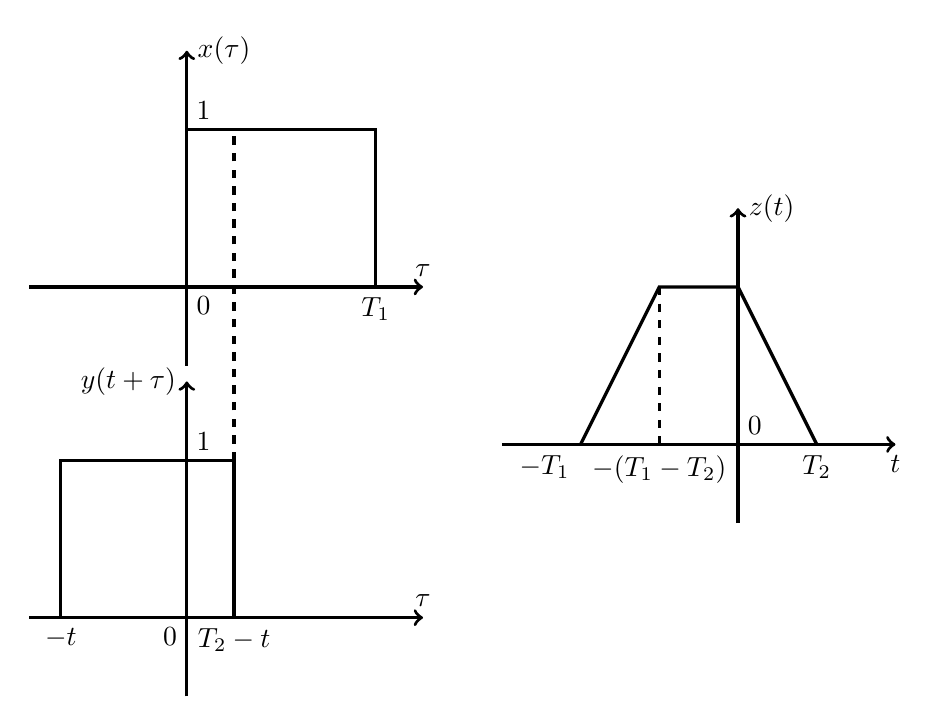
\begin{tikzpicture}[scale=2]
        \draw[->,very thick](-1,0)--(1.5,0)node[above]{$\tau$};
        \draw[->,very thick](0,-0.5)--(0,1.5)node[right]{$x(\tau)$};
        \node[below right]at(0,0){$0$};
        \node[above right]at(0,1){$1$};

        \draw[-,very thick](0,0)--(0,1)--(1.2,1)--(1.2,0)node[below]{$T_1$};

        \draw[->,very thick](-1,-2.1)--(1.5,-2.1)node[above]{$\tau$};
        \draw[->,very thick](0,-2.6)--(0,-0.6)node[left]{$y(t+\tau)$};
        \node[below left]at(0,-2.1){$0$};
        \node[above right]at(0,-1.1){$1$};

        \draw[-,very thick](0.3,-2.1)node[below]{$T_2-t$}--(0.3,-1.1)--(-0.8,-1.1)--(-0.8,-2.1)node[below]{$-t$};
        \draw[dashed,very thick](0.3,-1.1)--(0.3,1);


        \draw[->,very thick](2,-1)--(4.5,-1)node[below]{$t$};
        \draw[->,very thick](3.5,-1.5)--(3.5,0.5)node[right]{$z(t)$};
        \node[above right]at(3.5,-1){$0$};
        \draw[-,very thick](2.5,-1)node[below left]{$-T_1$}--(3,0)--(3.5,0)--(4,-1)node[below]{$T_2$};
        \draw[dashed, very thick](3,0)--(3,-1)node[below]{$-(T_1-T_2)$};
    \end{tikzpicture}
\end{center}

\subsection{Sistema Ingresso-Uscita}

Un sistema di ingress-uscita applica determinate trasformazioni al segnale $x$ in entrata, per ottenere un altro segnale $y$ in uscita, questo segnale è un funzionale 
del segnale di ingresso $y(t)=\mathscr{F}\{x(t)\}$. Questa trasformazione si basa su dei parametri interni $\sum$ al sistema per cui passa l'ingresso. 
\begin{center}
    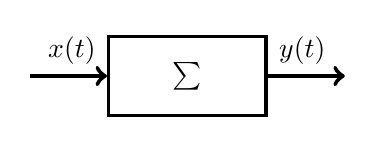
\begin{tikzpicture}[scale=2]
        \node[block](s){$\sum$};
        \draw[->,ultra thick](-1,0)--(s.180)node[above left]{$x(t)$};
        \draw[->,ultra thick](s.0)node[above right]{$y(t)$}--(1,0);
    \end{tikzpicture}
\end{center}

Un sistema ingresso-uscita si definisce lineare, se ad una combinazione lineare degli ingressi, corrisponde una combinazione lineare delle uscite:
\begin{equation*}
    x(t)=a_1(t)x_1(t)+\cdots+a_n(t)x_n(t)\to y(t)=b(t)_1y_1(t)+\cdots+b_n(t)y_n(t)
\end{equation*}

Un amplificatore rappresenta un sistema lineare, poiché moltiplica di un fattore $A$ un segnale in entrata:
\begin{gather*}
    x_1(t)\to y_1(t)=Ax_1(t)\\
    x_2(t)\to y_2(t)=Ax_2(t)\\
    ax_1(t)+bx_2(t)\to ay_1(t)+by_2(t)=A(ax_1(t)+bx_2(t))
\end{gather*} 
\begin{center}
    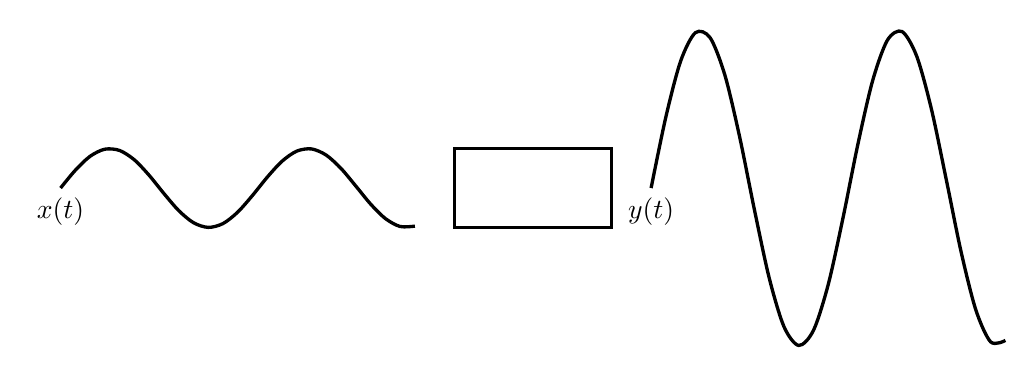
\begin{tikzpicture}[scale=2]
        \draw[-,very thick]plot[smooth, domain=-3:-0.75](\x,{0.25*sin(5*(\x+3) r)});
        \draw[-,very thick]plot[smooth, domain=0.75:3](\x,{1*sin(5*(\x-0.75) r)});
        \node[block](s)at(0,0){};
        \node[below]at(-3,0){$x(t)$};
        \node[below]at(0.75,0){$y(t)$};
    \end{tikzpicture}
\end{center}
Un sistema lineare non distorce gli ingressi. Un sistema che restituisce il segnale originario sommato per una costante $A$ non è lineare:
\begin{gather*}
    x(t)\to y(t)=x(t)+A\\
    x_1(t)+x_2(t)\to y(t)=x_1(t)+x_2(t)+A\neq y_1(t)+y_2(t)
\end{gather*}


Un sistema tempo invariante o permanente, non dipende da quando viene inserito il segnale in entrata:
\begin{gather*}
    x(t)\to y(t)\\
    x(t-\tau)\to y(t-\tau)
\end{gather*}
La linearità e la permanenza sono due proprietà indipendenti tra di loro. Un sistema può essere lineare e non pemanente e viceversa, oppure nessuno delle due. 
L'operazione di modulazione di un segnale, il prodotto tra l'entrata ed una funzione sinusoidale, è un sistema lineare e non permanente:
\begin{gather*}
    x(t)\to y(t)=x(t)\cos\displaystyle\left(\frac{2\pi t}{T}\right)\\
    x(t-\tau)\to y(t-\tau)=x(t-\tau)\displaystyle\cos\left(\frac{2\pi t}{T}\right)\neq x(t-\tau)\cos\left(\frac{2\pi (t-\tau)}{T}\right)
\end{gather*}
Per cui dipende dall'istante di tempo quando viene inserito il segnale. 


Un sistema può presentare un'altra proprietà chiamata causalità, che presenta un senso fisico. Un sistema si definisce causale se per ogni uscita all'istante $t_0$, dipende 
da valori entrate al massimo fino al tempo $t_0$: 
\begin{equation*}
    y(t_0)\propto x(t),\,\,t\leq t_0
\end{equation*}
L'uscita non può dipendere da entrate future, se il sistema è causale.
Data un'uscita $y$ dipendente dall'entrata $x$ traslata di un fattore $\tau$ $y(t)=x(t+\tau)$, se questo fattore di traslazione $\tau$ è negativo, l'uscita dipende da entrate ritardate 
per cui dipende da entrate passate, mentre se il fattore $\tau$ è positivo l'uscita dipende da entrate anticipate, quindi per un certo istante $t$ l'uscita dipende da entrate 
future. 


La linearità e la permanenza sono due proprietà fondamentali per cui un sistema si identifica come filtro, o SLI, Sistema Lineare Invariante. L'uscita di un filtro dipende 
solo da una funzione $h(t)$, chiamata risposta impulsiva, e si ottiene mediante la convoluzione tra l'entrata e quest'ultima:
\begin{equation*}
    x(t)\to y(t)=x(t)*h(t)
\end{equation*}
Si chiama risposta impulsiva, poiché se è presente un impulso in entrata, l'uscita è la funzione $h(t)$ stessa, per la proprietà della convoluzione di un impulso:
\begin{equation*}
    \delta(t)\to y(t)=\delta(t)*h(t)=h(t)
\end{equation*}

Per dimostrare l'uscita di un filtro, si considera il segnale $x$ come la somma integrale di impulsi moltiplicati per il valore della funzione in $x(\tau)$, ovvero la sua 
convoluzione:
\begin{gather*}
    x(t)=x(t)*\delta(t)=\displaystyle\int_{-\infty}^{+\infty}x(\tau)\delta(t-\tau)d\tau=\int_{-\infty}^{+\infty}dx(t)\\
\end{gather*}
Poiché il filtro è lineare si può considerare l'uscita $y$ come la somma integrale di tutte le uscite $dy$ per ogni entrata $dx=x(\tau)\delta(t-\tau)d\tau$. Poiché il fattore 
$x(\tau)$ non dipende dal tempo si considera una costante, per cui l'uscita $dy$ uguale al prodotto tra la costante $x(\tau)$ per la convoluzione tra l'impulso e la 
rispsosta impulsiva:
\begin{gather*}
    dx(t)=x(\tau)\delta(t-\tau)d\tau\\
    dy(t)=x(\tau)(\delta(t-\tau)*h(t))d\tau=x(\tau)h(t-\tau)d\tau
\end{gather*}
L'uscita totale si ottiene integrando su tutti i reali l'uscita infinitesima $dy(t)$:
\begin{equation*}
    y(t)=\displaystyle\int_{-\infty}^{+\infty}dy(t)=\int_{-\infty}^{+\infty}x(\tau)h(t-\tau)d\tau=x(t)*h(t)
\end{equation*}
Per cui l'uscita di un filtro corrisponde alla convoluzione tra l'entrata e la sua risposta impulsiva. 

Per determinare la risoluzione di uno schermo, dispostivo che opera come un filtro, si inserisce in entrata un impulso bidimensionale, rappresentato come un singolo punto 
su una superficie. L'uscita di questa entrata risulta in una macchia, più questa macchia, formata da vari pixel, è piccola maggiore è la risoluzione del dato schermo.  



Nel tempo discreto un sistema può essere caratterizzato dalle stesse propriettà. 
Linearità:
\begin{gather*}
    x_1[n]\to y_1[n]\\
    x_2[n]\to y_2[n]\\
    a_1x_1[n]+a_2x_2[n]\to a_1y_1[n]+a_2y_2[n]
\end{gather*}
Tempo invariante:
\begin{gather*}
    x[n+N]\to y[n+N]
\end{gather*}
Causalità:
\begin{equation*}
    y[n_0]\propto x[n],\,\, n\leq n_0
\end{equation*}
Si può esprimere formalmente questa condizione di causalità considerando un filtro con una risposta impulsiva $h[n]$:
\begin{equation*}
    y[n]=\displaystyle\sum_{k=-\infty}^{+\infty}x[k]h[n-k]
\end{equation*} 
Se questo filtro fosse causale allora la variabile $k$ non potrebbe superare il valore $n$, poiché ciò implicherebbe che l'uscita dipenda da entrate future:
\begin{equation*}
    y[n]=\displaystyle\sum_{k=-\infty}^nx[k]h[n-k]
\end{equation*}
Inoltre la risposta impulsiva deve essere nulla se il valore di $k$ è maggiore di $n$:
\begin{equation*}
    h[n-k]=0,\,\, k>n\to^{n-k=N}\to h[N],\,\, N<0
\end{equation*} 
Si può attuare lo stesso ragionamento per la causalità a tempo continuo. Un filtro è causale solo se:
\begin{gather*}
    y(t)=\displaystyle\int_{-\infty}^{+\infty}x(\tau)h(t-\tau)d\tau\to \int_{-\infty}^{+\infty}x(\tau)h(t-\tau)d\tau\\
    h(t-\tau)=0,\,\, \tau>t\to^{t-\tau=T}\to h(T)=0,\,\, T<0
\end{gather*}
Per cui:
\begin{equation*}
    y(t):\mbox{ causale}\iff \begin{cases}
        h[n]=0& n<0\\
        h(t)=0& t<0
    \end{cases}
\end{equation*}


Un filtro operante su tempo discreto viene definito, come nel contiuo, da un'unica funzione risposta impulsiva $h[n]$:
\begin{equation*}
    \delta[n]*h[n]=h[n]
\end{equation*}
Si esprime per la proprietà di campionamento dell'impulso, un qualsiasi segnale $x$ come:
\begin{equation*}
    x[n]=\displaystyle\sum_{k=-\infty}^{+\infty}x[k]\delta[n-k]
\end{equation*}
Poiché il filtro è un sistema lineare, si possono considera le singole entrate della sommatoria e poi sommare le loro uscite corrispondenti per ottenere l'uscita complessiva. 
Si considera l'uscita per un qualsiasi $k$, pari alla convoluzione tra l'impulso $\delta[n-k]$ e la risposta impulsiva $h[n]$, si considera il parametro $x[k]$ costante poiché 
non dipende dalla variabile $n$:
\begin{equation*}
    y_k[n]=x[k](\delta[n-k]*h[n])=x[k]h[n-k]
\end{equation*}
La somma su tutti gli interi di questo valore $y_k$ corrisponde all'uscita totale $y$ del sistema per l'entrata $x$:
\begin{equation*}
    y[n]=\displaystyle\sum_{k=-\infty}^{+\infty}y_k[n]=\sum_{k=-\infty}^{+\infty}x[k]h[n-k]=x[n]*h[n]
\end{equation*}
Questa uscita $y$ corrisponde alla convoluzione tra l'entrata $x$ e la risposta impulsiva $h$. 


Data la struttura del sistema è possibile individuare l'uscita in forma analitica rispetto ad una generica entrata. Dopo aver determinaro la risposta impulsiva inserendo 
al posto di una generica entrata $x$ l'impulso $\delta$, è possibile sostituire l'intero modello strutturale del sistema con un singolo blocco funzionale, un'oggetto che 
applica all'entrata la convoluzione per i parametri contenuti, contenente la risposta impulsiva.  
Si considera un generico schema di un circuito sommatore, un tipo di sistema controllore a feedforward:
\begin{center}
    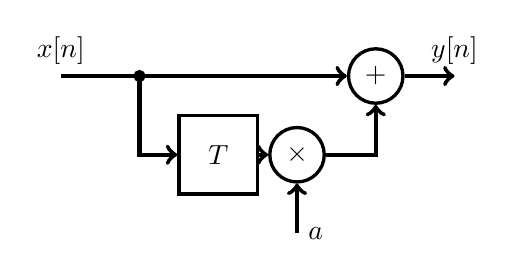
\begin{tikzpicture}[scale=2]
        \node[sum](+)at(2,0){$+$};
        \draw[->,ultra thick](0,0)node[above]{$x[n]$}--(+.180);
        \filldraw[black](0.5,0)circle(1pt);

        \node[square](t)at(1,-0.5){$T$};
        \draw[->,ultra thick](0.5,0)--(0.5,-0.5)--(t.180);

        \node[sum](x)at(1.5,-0.5){$\times$};
        \draw[->,ultra thick](t.0)--(x.180);
        \draw[->,ultra thick](1.5,-1)node[right]{$a$}--(x.270);

        \draw[->,ultra thick](x.0)--(2,-0.5)--(+.270);
        \draw[->,ultra thick](+.0)--(2.5,0)node[above]{$y[n]$};
    \end{tikzpicture}
\end{center}
Per ottenere l'uscita si somma il segnale originario per lo stesso segnale ritardato di un campione e moltiplicato per un fattore $a$:
\begin{gather*}
    y[n]=x[n]+ax[n-1]\\
    h[n]=\delta[n]+a\delta[n-1]
\end{gather*}
\begin{center}
    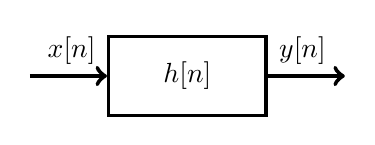
\begin{tikzpicture}[scale=2]
        \node[block](s){$h[n]$};
        \draw[->,ultra thick](-1,0)--(s.180)node[above left]{$x[n]$};
        \draw[->,ultra thick](s.0)node[above right]{$y[n]$}--(1,0);
    \end{tikzpicture}
\end{center}

\clearpage

\section{Espansione di Fourier}

Dati due segnali in frequenza doppia come il La$4$ a $\approx 440Hz$ ed il La$5$ a $\approx 880Hz$, non si nota la differenza poiché sono esattamente una il doppio dell'altra. 
In genera segnali musicali affinché suonino bene devono avere frequenze tra di loro o multipli oppure relati da frazioni semplici, non possono essere scelte arbitrariamente. 
Queste frequenze sono associate a varie note, inserendo una serie di queste note è possible scrivere un segnale musicale. Viene attuato un processo analogo tramite la serie di 
Fuorier. Questo tipo di analisi venne introdatta da Fouriere nella sua teoria analitica del calore, dove oltre all'omonima serie e trasformata, introdusse molti concetti 
matematici importanti. 



La serie di Fourier è uno strumento per esprimere solo i segnali periodici, 
se il segnale non è periodico si usa la trasformata di Fourier, se rispetta le condizioni di Dirichlet, ma per i nostri fini si considerano sempre verificate. 
I segnali si esprimono rispetto alle sue armoniche. Dato un segnale $x(t)$ di periodo $T$, può essere rappresentato come una serie, ovvero una sommatoria, di alcuni 
coefficienti di Fourier per un fattore esponenziale, chiamato armonica, di frequenza multiplo della frequenza del segnale originario:
\begin{equation*}
    x(t)=\displaystyle\sum_{k=-\infty}^{+\infty}c_ke^{i\frac{2\pi  k t}{T}}
\end{equation*}
Il fattore $c_k$ indica se una data frequenza è presente nel segnale analizzato. Le armoniche sono note a priori, dal punto di vista fisico non esistono armoniche di frequenze 
negative, ma in ambito matematico sono necessarie per esprimere il segnale. Considerando la rappresentazione di Eulero si può esprimere la serie di Fourier come:
\begin{equation*}
    x(t)=\displaystyle\sum_{k=-\infty}^{+\infty}c_k\left[\cos\left(\frac{2\pi k t}{T}\right)+i\sin\left(\frac{2\pi k t}{T}\right)\right]
\end{equation*}
Poiché le armoniche sono le stesse, l'unica differenza tra varie rappresentazioni di Fourier è il valore dei coefficienti $c_k$ assegnati. Lo spazio dei segnali periodici, 
aventi lo stesso periodo $T$, può essere scritto come uno spazio vettoriale dotato di prodotto scalare, dove ogni segnale è espresso come un vettore. Questo spazio può essere 
espresso data una base ortonormale.

\subsection{Spazio Vettoriale}

Dato uno spazio euclideo $\mathbb{R}^3$ descritto da tre vettori ortonormali $\hat x=(1,0,0)$, $\hat y=(0,1,0)$ e $\hat z=(0,0,1)$, chiamati base canonica dello spazio vettoriale. 
Dei vettori di uno spazio vettoriale si dicono base, se sono ortonormali tra di loro, quindi il prodotto scalare tra di loro è nullo ovvero sono linearmente indipendenti, 
mentre si dicono basi canoniche se il quadrato di un vettore, il prodotto scalare per sé stesso, equivale ad uno. 
Il prodotto scalare è un'operazione binaria interna ad uno spazio vettoriale $V$ che resitituisce uno scalare:
\begin{equation*}
    \langle \cdot \; , \; \cdot \rangle : V \times V  \rightarrow \mathbb{R}
\end{equation*}
Si definisce come il prodotto matriciale tra il primo vettore per la trasposta del secondo:
\begin{equation*}
    \langle\vec v,\,\vec w\rangle=\vec v\cdot \vec w^T=\begin{pmatrix}
        v_x &v_y&v_z
    \end{pmatrix}\cdot\begin{pmatrix}
        w_x\\ w_y \\ w_z
    \end{pmatrix}
\end{equation*} 
Per ottenere una certa componente di un generico vettore $\vec{v}$ si considera il prodotto tra quel vettore e la base della componente desiderata:
\begin{equation*}
    \langle\vec v,\,\hat x\rangle=\vec v\cdot \hat x^T=\begin{pmatrix}
        v_x &v_y&v_z
    \end{pmatrix}\cdot\begin{pmatrix}
        1\\ 0 \\0
    \end{pmatrix}=v_x
\end{equation*} 



Il segnale periodico $x(t)$ può essere scritto come una somma di coefficienti moltiplicati per una base ortonormale dello spazio vettoriale dei segnali periodici di periodo 
$T$. In questo spazio sono presenti infiniti vettori ortonormali tra di loro, a differenza dello spazio euclideo $\mathbb{R}^3$, dove sono presenti tre vettori base. Questo 
spazio è quindi uno spazio euclideo di dimensione numerabile, ma infinita, poiché le basi ortonormali corrispondono alle infinite armoniche di periodo $T$. 
Il prodotto scalare tra due segnali $x$ e $y$ viene definito come:
\begin{equation*}
    \langle x(t),\,y(t)\rangle=x(t)\cdot y(t)=\displaystyle\int_{-\infty}^{+\infty}x(t)\cdot y^*(t)dt
\end{equation*}
Il prodotto scalare tra due segnali periodici viene definito come:
\begin{equation*}
    \langle x(t),\,y(t)\rangle=x(t)\cdot y(t)=\displaystyle\frac{1}{T}\int_{-\frac{T}{2}}^{\frac{T}{2}}x(t)\cdot y^*(t)dt
\end{equation*}
Per cui per ottenere i coefficienti di Fourier $c_k$ rispetto ad una determinata armonica $k$ di un segnale $x$ si considera il prodotto scalare tra quel segnale per l'
armonica $k$:
\begin{equation*}
    c_k=\langle x(t),\,e^{i\frac{2\pi  k t}{T}}\rangle=\displaystyle\frac{1}{T}\int_{-\frac{T}{2}}^{\frac{T}{2}}x(t)\cdot e^{-i\frac{2\pi  k t}{T}}dt
\end{equation*} 

Il prodotto tra due basi è nullo, tranne nel caso dove sono la stessa base, in quel caso il risultato è $1$. Per dimostrare che le armoniche rappresentano una base dello 
spazio vettoriale si considera il prodotto scalare tra un'armonica $k$ ed una $l$:
\begin{gather*}
    \langle e^{i\frac{2\pi kt}{T}},e^{i\frac{2\pi lt}{T}}\rangle=\displaystyle\frac{1}{T}\int_{-\frac{T}{2}}^{\frac{T}{2}}e^{i\frac{2\pi kt}{T}}e^{-i\frac{2\pi lt}{T}}dt=
    \frac{1}{T}\left[e^{i\frac{2\pi(k-l)t}{T}}\frac{T}{2i\pi (k-l)}\right]^{\frac{T}{2}}_{-\frac{T}{2}}\\
    \displaystyle\frac{e^{i\pi(l-k)}-e^{-i\pi(l-k)}}{2i}\frac{1}{\pi (k-l)}=\frac{\sin(\pi(k-l))}{\pi (k-l)}
\end{gather*} 
Questa funzione risulta essere una sinc, e per definizione è un segnale che si annulla per ogni valore intero, e poiché $k$ e $l$ sono due interi la loro differenza lo è 
poiché l'insieme degli interi è chiuso rispetto alla somma: $k-l\in\mathbb{Z}$. Quindi il prodotto scalare tra due armoniche $k$ e $l$, non triviale: $k\neq l$, è di valore 
nullo:
\begin{equation*}
    \forall k\neq l\in\mathbb{Z}\implies \langle e^{i\frac{2\pi kt}{T}},e^{i\frac{2\pi lt}{T}}\rangle=0
\end{equation*}
\'{E} stato dimostrato che le armoniche sono una base dello spazio vettoriale dei segnali periodici di periodo $T$. 
Per $k=0$ l'armonica corrispondente è un segnale costante. In generale un'armonica di ordine $k$ si può esprimere mediante la rappresentazione di Eulero:
\begin{equation*}
    \displaystyle e^{i\frac{2\pi kt}{T}}=\cos\left(\frac{2\pi kt}{T}\right)+i\sin\left(\frac{2\pi kt}{T}\right)
\end{equation*}
Per cui la parte reale di un'armonica oscilla come un segnale coseno di frequenza dell'armonica. 

\subsection{Serie Elementari}

Si considera un segnale costante $x(t)=A$. Per determinare i coefficienti della sua serie di Taylor si considera il prodotto scalare tra il segnale ed una generica armonica $k$: 
\begin{gather*}
    c_k=\langle x(t),e^{i\frac{2\pi kt}{T}}\rangle=\displaystyle\frac{1}{T}\int_{-\frac{T}{2}}^{\frac{T}{2}}Ae^{-i\frac{2\pi kt}{T}}dt=\left[A\frac{e^{-i\frac{2\pi kt}{T}}}{-2i\pi k}\right]_{-\frac{T}{2}}^{\frac{T}{2}}\\
    \displaystyle\frac{A(e^{-i\pi k}-e^{i\pi k})}{-2i\pi k}=A\frac{-\sin(\pi k)}{-\pi k}=A\,\mbox{sinc}[k]
\end{gather*}
L'unico valore per cui il seno cardinale discreto in funzione di $k$ assume un valore non nullo è per $k=0$:
\begin{equation*}
    c_0=A\,\cancelto{1}{\mbox{sinc}[0]}\to x(t)=c_0e^{\cancelto{0}{i\frac{2\pi kt}{T}}}
\end{equation*}

Si considera un coseno di periodo $T$: $x(t)=A\cos\left(\frac{2\pi t}{T}\right)$. Si vuole determinare la sua espansione di Fourier, per cui si considera il suo prodotto 
scalare con una generica armonica $k$. Si esprime il coseno tramite le formule di Eulero, in questo modo assume la stessa forma di una differenze di due armoniche: 
\begin{gather*}
    c_k=\displaystyle\frac{1}{T}\int_{-\frac{T}{2}}^{\frac{T}{2}}A\cos\left(\frac{2\pi t}{T}\right)e^{-i\frac{2\pi kt}{T}}dt=
    \frac{A}{2T}\left(\int_{-\frac{T}{2}}^{\frac{T}{2}}e^{i\frac{2\pi t}{T}}e^{-i\frac{2\pi kt}{T}}dt+\int_{-\frac{T}{2}}^{\frac{T}{2}}e^{-i\frac{2\pi t}{T}}e^{-i\frac{2\pi kt}{T}}dt\right)
\end{gather*}
Il prodotto scalare tra due armoniche è stato precedentemente individuato come un seno cardinale:
\begin{equation*}
    \displaystyle c_k=\frac{A\,\mbox{sinc}[1-k]+A\,\mbox{sinc}[-(1+k)]}{2}
\end{equation*}
Il seno cardinale nel discreto assume gli stessi valori dell'impulso discreto. 
Quindi il coefficiente è nullo per ogni $k\neq1\lor-1$, gli unici coefficienti non nulli della sua serie di Fourier sono $c_{-1}$ e $c_1$:
\begin{gather*}
    \displaystyle c_1=c_{-1}=\frac{A}{2}\\
    \displaystyle x(t)=c_{-1}e^{-i\frac{2\pi t}{T}}+c_1e^{i\frac{2\pi t}{T}}
\end{gather*}


Si applica un processo analogo per determinare l'espansione di Fourier di un segnale sinusoidale $x(t)=\sin\left(\frac{2\pi t}{T}\right)$:
\begin{gather*}
    c_k=\displaystyle\frac{1}{T}\int_{-\frac{T}{2}}^{\frac{T}{2}}A\sin\left(\frac{2\pi t}{T}\right)e^{-i\frac{2\pi kt}{T}}dt=
    \frac{A}{2iT}\left(\int_{-\frac{T}{2}}^{\frac{T}{2}}e^{i\frac{2\pi t}{T}}e^{-i\frac{2\pi kt}{T}}dt-\int_{-\frac{T}{2}}^{\frac{T}{2}}e^{-i\frac{2\pi t}{T}}e^{-i\frac{2\pi kt}{T}}dt\right)\\
    \displaystyle c_k=\frac{A\,\mbox{sinc}[1-k]-A\,\mbox{sinc}[-(1+k)]}{2i}\\
    c_1=-c_{-1}=\frac{A}{2i}\\
    x(t)=c_{-1}e^{-i\frac{2\pi t}{T}}+c_1e^{i\frac{2\pi t}{T}}
\end{gather*}
Altrimenti è possible calcolare i coefficienti tramite confronto diretto dalla rappresentazione di Eulero delle funzioni trigonometriche, in questo modo si individuano le due 
armoniche che producono il segnale sinusoidale, di ordine $1$ e $-1$. 


Si considera ora un segnale $x(t)=A\cos^2\left(\frac{2\pi t}{T}\right)$. Per le fofmula di duplicazione del coseno si può riscrivere come:
\begin{equation*}
    A\cos^2\left(\frac{2\pi t}{T}\right)=\frac{A}{2}\left(\cos\left(\frac{4\pi t}{T}\right)+1\right)
\end{equation*}
Si calcola il valore di un coefficiente generico $k$:
\begin{gather*}
    c_k=\displaystyle\frac{1}{T}\int_{-\frac{T}{2}}^{\frac{T}{2}}A\cos^2\left(\frac{2\pi t}{T}\right)e^{-i\frac{2\pi kt}{T}}dt=
    \frac{A}{2T}\int_{-\frac{T}{2}}^{\frac{T}{2}}\left(\cos\left(\frac{4\pi t}{T}\right)+1\right)e^{-i\frac{2\pi kt}{T}}dt\\
    \displaystyle\frac{A}{2T}\left(\int_{-\frac{T}{2}}^{\frac{T}{2}}e^{i\frac{4\pi t}{T}}e^{-i\frac{2\pi kt}{T}}dt+\int_{-\frac{T}{2}}^{\frac{T}{2}}e^{-i\frac{4\pi t}{T}}e^{-i\frac{2\pi kt}{T}}dt+\int_{-\frac{T}{2}}^{\frac{T}{2}}e^{-i\frac{2\pi kt}{T}}dt\right)\\
    \displaystyle\frac{A}{2}\left(2\,\mbox{sinc}[2-k]-2\,\mbox{sinc}[-(2+k)]+\mbox{sinc}[k]\right)
\end{gather*}
I coefficienti non si annullano per valori di $k$ pari a $\pm2$ e $0$:
\begin{equation*}
    x(t)=c_{-2}e^{-i\frac{4\pi t}{T}}+c_0+c_2e^{i\frac{4\pi t}{T}}
\end{equation*}


Si considera un segnale onda quadra di periodo $T$ e di base $\tau$: 
\begin{equation*}
    x(t)=\displaystyle\sum_{n=-\infty}^{+\infty}\mbox{rect}\left(\frac{t-nT}{\tau}\right)
\end{equation*}
Si determina il valore di un coefficiente generico $k$:
\begin{gather*}
    c_k=\displaystyle\frac{1}{T}\int_{-\frac{T}{2}}^{\frac{T}{2}}\sum_{n=-\infty}^{+\infty}\mbox{rect}\left(\frac{t-nT}{\tau}\right)e^{-i\frac{2\pi k t}{T}}dt
\end{gather*}
Nell'intervallo $[-T/2,T/2]$ cade una sola finestra di base $\tau$, per $n=0$, per cui si può riscrivere come:
\begin{gather*}
    c_k=\displaystyle\frac{1}{T}\int_{-\frac{T}{2}}^{\frac{T}{2}}\mbox{rect}\left(\frac{t}{\tau}\right)e^{-i\frac{2\pi k t}{T}}dt=\frac{1}{T}\int_{-\frac{\tau}{2}}^{\frac{\tau}{2}}e^{-i\frac{2\pi k t}{T}}=
    \left[\frac{e^{-i\frac{2\pi kt}{T}}}{-2i\pi k}\right]_{-\frac{\tau}{2}}^{\frac{\tau}{2}}\\
    \displaystyle\frac{e^{-i\pi k\frac{\tau}{T}}-e^{i\pi k\frac{\tau}{T}}}{-2i}\frac{1}{\pi k}=\frac{\tau}{T}\frac{\sin\left(\frac{\pi k \tau}{T}\right)}{\frac{\pi k \tau}{T}}=\frac{\tau}{T}\mbox{sinc}\left(\frac{k \tau}{T}\right)
\end{gather*}

Il seno cardinale non è discreto, poiché l'argomento non necessariamente assume valore intero. 
\begin{equation*}
    x(t)=\displaystyle\sum_{n=-\infty}^{+\infty}\mbox{rect}\left(\frac{t-nT}{\tau}\right)=\sum_{k=-\infty}^{+\infty}\frac{\tau}{T}\mbox{sinc}\left(\frac{k \tau}{T}\right)e^{i\frac{2\pi kt}{T}}
\end{equation*}
All'aumentare di $k$ e quindi della frequenza delle armoniche, il valore dei coefficienti diminuisce, quindi diminuiscono anche i contributi che le armoniche a frequenza 
maggiore per la ricostruzione del segnale originale. I coefficienti rappresentano il peso di quanto le armoniche contribuiscono al segnale originario. La precisione 
aumenta sempre di meno per ogni nuova armonica aggiunta, fino a ricostruire completamente il segnale originale se $k$ tende asintoticamente ad infinito. Da notare che se 
$T=2\tau$, per $k$ pari i coefficienti della serie di Fourier dell'onda quadra che ha periodo esattamente il doppio della base sono nulli. In generale se $T=n\tau$, dove 
$n\in\mathbb{N}$, i contributi delle armoniche con frequenza multiplo di $n/T$ sono nulli, ovvero i coefficienti con $k$ multiplo di $n$ sono nulli:
\begin{gather*}
    c_k=\frac{1}{n}\mbox{sinc}\left(\frac{k}{n}\right)=0\;\forall k=\alpha\cdot n,\;\alpha\in\mathbb{Z}
\end{gather*}
In generale se $T/\tau\notin\mathbb{Z}$ e $\tau/T\notin\mathbb{Z}$, i coefficienti dell'espansione di Fourier non sono mai nulli, poiché non comprendono mai zeri triviali 
della funione seno cardinale. 

\subsection{Proprietà}

Cercare il periodo del segnale in alcuni casi, non specificato dal testo del problema. Il contenuto informativo del segnale è descritto dai coefficienti della serie di Fourier 
$c_k$. 

\subsubsection{Linearità}

Poiché segnali $x(t)$ e $y(t)$, periodici di periodo $T$, possono essere espresso come espansione di Fourier rispetto alle stesse armoniche, la loro combinazione lineare 
può essere espressa come una combinazione lineare dei coefficienti delle due espansioni di Fourier:
\begin{gather*}
    x(t)=\displaystyle\sum_{k=-\infty}^{+\infty}c_ke^{i\frac{2\pi  k t}{T}}\\    
    y(t)=\displaystyle\sum_{k=-\infty}^{+\infty}d_ke^{i\frac{2\pi  k t}{T}}\\
    ax(t)+by(t)=\displaystyle\sum_{k=-\infty}^{+\infty}(ac_k+bd_k)e^{i\frac{2\pi  k t}{T}}\\
    \displaystyle\frac{1}{T}\int_{-\frac{T}{2}}^{\frac{T}{2}}(ax(t)+by(t))dt=\frac{a}{T}\int_{-\frac{T}{2}}^{\frac{T}{2}}x(t)e^{-i\frac{2\pi  k t}{T}}dt
    +\frac{b}{T}\int_{-\frac{T}{2}}^{\frac{T}{2}}y(t)e^{-i\frac{2\pi  k t}{T}}dt=ac_k+bd_k
\end{gather*}

Data un'onda quadra $z(t)$ che assume valori di $1$ e $-1$ periodicamente, con periodo $T$, può essere espressa come una differenza tra due onde quadre $x(t)$ e $y(t)$ in 
opposizione di fase che assumono valori di $1$ e $0$ con periodo $T$. Una delle quali ha una base di lunghezza $\tau$, mentre l'altra lunghezza di $T-\tau$ e traslata di un 
semiperiodo $T/2$:
\begin{equation*}
    z(t)=\displaystyle\sum_{k=-\infty}^{+\infty}\left[\mbox{rect}\left(\frac{t-kT}{\tau}\right)-\mbox{rect}\left(\frac{t-nT-\frac{T}{2}}{T-\tau}\right)\right]
\end{equation*}

\begin{center}
    \begin{tikzpicture}[scale=2]
        \draw[->](-2.5,0)--(2.5,0)node[above]{$t$};
        \draw[->](0,-1)--(0,1)node[right]{$z(t)$};
        \draw[-](-2.5,0.5)--(-2,0.5)--(-2,-0.5)--(-0.5,-0.5)--(-0.5,0.5)--(0.5,0.5)--(0.5,-0.5)--(2,-0.5)--(2,0.5)--(2.5,0.5);
        \node[above right]at(0,0.5){$1$};
        \node[below right]at(0,-0.5){$-1$};
    \end{tikzpicture}
\end{center}

Si calcolano ora i coefficienti dell'espansione di Fourier:
\begin{gather*}
    a_k=\displaystyle\frac{1}{T}\int_{-\frac{T}{2}}^{\frac{T}{2}}\left[\mbox{rect}\left(\frac{t-kT}{\tau}\right)-\mbox{rect}\left(\frac{t-kT-\frac{T}{2}}{T-\tau}\right)\right]dt\\
    \displaystyle\frac{1}{T}\int_{-\frac{\tau}{2}}^{\frac{\tau}{2}}\mbox{rect}\left(\frac{t-kT}{\tau}\right)dt-\frac{1}{T}\int_{-\frac{T-\tau}{2}}^{\frac{T-\tau}{2}}\mbox{rect}\left(\frac{t-kT-\frac{T}{2}}{T-\tau}\right)dt\\
    \displaystyle\frac{e^{-i\pi k\frac{\tau}{T}}-e^{i\pi k\frac{\tau}{T}}}{-2i}\frac{1}{\pi k}\frac{\tau}{T}-\frac{e^{-i2\pi k\frac{T-\tau/2}{T}}-e^{i2\pi k\frac{T-\tau/2}{T}}}{-2i}\frac{1}{\pi k}\frac{\tau}{T}
\end{gather*}
Per $k=0$ si ottiene una forma indeterminata, per cui bisogna risolvere l'integrale considerando il valor medio assunto dal segnale nell'intervallo $\left[-T/2,T/2\right]$. 
\begin{gather*}
    \displaystyle\frac{\tau}{T}\mbox{sinc}\left(\frac{k\tau}{T}\right)-\frac{e^{i\pi k\frac{\tau}{T}}-e^{-i\pi k\frac{\tau}{T}}}{-2i}\frac{1}{\pi k}\\
    c_k=\displaystyle\frac{2\tau}{T}\mbox{sinc}\left(\frac{k\tau}{T}\right)
\end{gather*}


Generalmente si differenziano i casi dove l'esponeniale assume valore unitario, per $k=0$, dai casi dove è presente un'armonica generica. 

Il segnale originale può essere espresso come un'onda quadra doppia, di stesso periodo $T$ e base $\tau$, e traslata verso il basso:
\begin{equation*}
    z(t)=\displaystyle\sum_{k=-\infty}^{+\infty}\left[2\,\mbox{rect}\left(\frac{t-kT}{\tau}\right)\right]-1=2x(t)-1
\end{equation*}
In questo modo si effettuano meno calcoli per determinare i coefficienti di Fourier, usufruendo della proprietà di linearità bisogna tenere conto che il fattore costante $-1$, 
assume un valore non nullo solo per $k=0$. Si considerano i coefficienti del segnale $x$ come $c_k$, mentre del segnale costante $d_k$, per cui in questo caso i coefficienti 
del segnale $z$ si esprimono come: 
\begin{equation*}
    a_k=\begin{cases}
        2c_k+d_k &k=0\\
        2c_k&k\neq0
    \end{cases}=\begin{cases}
        \displaystyle\frac{2\tau}{T}-1&k=0\\
        \displaystyle\frac{2\tau}{T}\mbox{sinc}\left(\frac{k\tau}{T}\right)&k\neq0
    \end{cases}
\end{equation*}

\subsubsection{Traslazione nel Tempo}

Si considera un segnale ritardato nel tempo di un fattore $t_0$: $x(t-t_0)$, dati i coefficienti del segnale non traslato $c_k$. Per confronto diretto si ottiene:
\begin{gather*}
    x(t)=\displaystyle\sum_{k=-\infty}^{+\infty}c_ke^{i\frac{2\pi kt}{T}}\\
    x(t-t_0)=\displaystyle\sum_{k=-\infty}^{+\infty}c_ke^{i\frac{2\pi k(t-t_0)}{T}}=\sum_{k=-\infty}^{+\infty}\left(c_ke^{-i\frac{2\pi kt_0}{T}}\right)e^{i\frac{2\pi kt}{T}}\\
    x(t-t_0)=\displaystyle\sum_{k=-\infty}^{+\infty}d_ke^{i\frac{2\pi kt}{T}}
\end{gather*}
Per cui tutti i coefficienti equivalgono ai coefficienti non traslati $c_k$ moltiplicati per un fattore esponenziale, che dipende dalla traslazione $t_0$:
\begin{equation*}
    \displaystyle d_k=c_ke^{-i\frac{2\pi kt_0}{T}}
\end{equation*}

Altrimenti si possono determinare i coefficienti tramite la definizione, attuando una sostituzione $t-t_0\to\tau$:
\begin{gather*}
    d_k=\displaystyle\frac{1}{T}\int_{-\frac{T}{2}}^{\frac{T}{2}}x(t-t_0)e^{-i\frac{2\pi kt}{T}}dT\to\int_{-\frac{T}{2}-t_0}^{\frac{T}{2}-t_0}x(\tau)e^{-i\frac{2\pi kt_0}{T}}e^{-i\frac{2\pi k\tau}{T}}d\tau\\
    d_k=\displaystyle\frac{1}{T}e^{-i\frac{2\pi kt_0}{T}}\int_{-\frac{T}{2}-t_0}^{\frac{T}{2}-t_0}x(\tau)e^{-i\frac{2\pi k\tau}{T}}d\tau=\frac{1}{T}e^{-i\frac{2\pi kt_0}{T}}c_k
\end{gather*}
Dove $c_k$ sono i coefficienti del segnale non traslato. 


%grafico(?)
% EX:
Si considera un'onda quadra di periodo $T$ traslata di un fattore $\tau$, corrispondente alla lunghezza della sua base. Dati i coefficienti di un onda quadra non traslata 
$c_k$ si possono esprimere direttamente i coefficienti del segnale traslato $d_k$:
\begin{equation*}
    d_k=\displaystyle\frac{\tau}{T}\mbox{sinc}\left(\frac{k\tau}{T}\right)e^{-i\frac{2\pi k\tau}{T}}
\end{equation*}

In caso il periodo sia esattamente il doppio della base $T=2\tau$:
\begin{equation*}
    d_k=\displaystyle\frac{1}{2}\mbox{sinc}\left(\frac{k}{2}\right)e^{-i\pi k}=\frac{1}{2}\frac{e^{i\frac{\pi k}{2}}-e^{-i\frac{\pi k}{2}}}{i\pi k}e^{-i\pi k}=
    \frac{e^{-i\frac{\pi k}{2}}-e^{-i\frac{3\pi k}{2}}}{2i\pi k}
\end{equation*}
Per cui i coefficienti dell'onda quadra di armoniche di ordine pari risultano nulli. 

\subsubsection{Traslazione in Frequenza}

Si considera un segnale $x$ moltiplicato per un'armonica di ordine $n$:
\begin{equation*}
    y(t)=x(t)\cdot e^{i\frac{2\pi nt}{T}}=\displaystyle\sum_{k=-\infty}^{+\infty}c_ke^{i\frac{2\pi kt}{T}}e^{i\frac{2\pi nt}{T}}=\sum_{k=-\infty}^{+\infty}c_ke^{i\frac{2\pi (k+n)t}{T}}
\end{equation*}
Si considera la sotituzione $l=n+k$:
\begin{equation*}
    y(t)=\displaystyle\sum_{l=-\infty}^{+\infty}c_{l-n}e^{i\frac{2\pi lt}{T}}
\end{equation*}

Per cui i coefficienti dell'espansione di Fourier di $y$, corrispondo agli stessi coefficienti del segnale originario $x$, ma ad un generico coefficienti $c_k$ viene 
associata l'armonica di ordine $k+n$.   
Tramite la definizione integrale dei coefficienti di Fourier, si arriva allo stesso risultato:
\begin{gather*}
    \langle y(t),\;e^{i\frac{2\pi kt}{T}}\rangle=\displaystyle\frac{1}{T}\int_{-\frac{T}{2}}^{\frac{T}{2}}\left(x(t)\cdot e^{i\frac{2\pi nt}{T}}\right)e^{-i\frac{2\pi kt}{T}}dt=\frac{1}{T}\int_{-\frac{T}{2}}^{\frac{T}{2}}x(t)\left(e^{i\frac{2\pi nt}{T}}e^{-i\frac{2\pi kt}{T}}\right)dt\\
    \displaystyle\frac{1}{T}\int_{-\frac{T}{2}}^{\frac{T}{2}}x(t)e^{i\frac{2\pi (n-k)t}{T}}dt=d_k=c_{k-n}
\end{gather*}
Si ottiene lo stesso risultato, i coefficienti associati alle armoniche vengono traslati di un fattore $n$, fattore del ritardo in frequenza del segnale.  

\subsubsection{Teorema della Modulazione}

Quando un segnale viene moltiplicato per un conseno ad una determinata frequenza si indica quest'operazione come modulazione. 
\begin{gather*}
    y(t)=x(t)\cos\displaystyle\left(\frac{2\pi t}{T}\right)=x(t)\left[\frac{e^{i\frac{2\pi t}{T}}+e^{-i\frac{2\pi t}{T}}}{2}\right]=\sum_{k=-\infty}^{+\infty}c_ke^{i\frac{2\pi kt}{T}}\frac{e^{i\frac{2\pi t}{T}}+e^{-i\frac{2\pi t}{T}}}{2}\\
    y(t)=\displaystyle\frac{1}{2}\sum_{k=-\infty}^{+\infty}c_ke^{i\frac{2\pi (k+1)t}{T}}+\frac{1}{2}\sum_{k=-\infty}^{+\infty}c_ke^{i\frac{2\pi (k-1)t}{T}}=\frac{1}{2}\left(\sum_{m=-\infty}^{+\infty}c_{m-1}e^{i\frac{2\pi mt}{T}}+\sum_{m=-\infty}^{+\infty}c_{m+1}e^{i\frac{2\pi mt}{T}}\right)\\
    d_k=\displaystyle\frac{1}{2}c_{k-1}+\frac{1}{2}c_{k+1}
\end{gather*}

\subsubsection{Teroema della Derivazione}

Espansione di Fourier della derivata di un segnale $x(t)$:
\begin{gather*}
    y(t)=\displaystyle\frac{d}{dt}x(t)=\frac{d}{dt}\left(\displaystyle\sum_{k=-\infty}^{+\infty}c_ke^{i\frac{2\pi kt}{T}}\right)=\sum_{k=-\infty}^{+\infty}c_k\frac{2i\pi k}{T}e^{i\frac{2\pi kt}{T}}\\
    d_k=c_k\displaystyle\frac{2i\pi k}{T}
\end{gather*}
Tramite la definizione, si risolve tramite integraazione per parti:
\begin{gather*}
    d_k=\displaystyle\frac{1}{T}\int_{-\frac{T}{2}}^{\frac{T}{2}}\frac{d}{dt}x(t)e^{-i\frac{2\pi kt}{T}}dt=
    \left[\frac{1}{T}x(t)e^{-i\frac{2\pi kt}{T}}\right]_{-\frac{T}{2}}^{\frac{T}{2}}+\frac{1}{T}\int_{-\frac{T}{2}}^{\frac{T}{2}}x(t)\frac{2i\pi k}{T}e^{-i\frac{2\pi kt}{T}}dt\\
    \displaystyle-\frac{1}{T}x(t)\left(e^{i\pi k}-e^{-i\pi k}\right)+c_k\frac{2i\pi k}{T}\\
    \displaystyle-\frac{2i}{T}\cancelto{0}{\sin(\pi k)}+c_k\frac{2i\pi k}{T}\\
    d_k=c_k\displaystyle\frac{2i\pi k}{T}
\end{gather*}

\subsubsection{Teorema di Perceval}

Questo teorema permette di calcolare velocemente la potenza di un segnale periodico, la potenza di un segnale periodico è definita come:
\begin{gather*}
    P_x=\displaystyle\frac{1}{T}\int_{-\frac{T}{2}}^{\frac{T}{2}}x(t)x^*(t)dt=
    \frac{1}{T}\int_{-\frac{T}{2}}^{\frac{T}{2}}\left(\sum_{k=-\infty}^{+\infty}c_ke^{i\frac{2\pi kt}{T}}\right)\cdot\left(
    \sum_{n=-\infty}^{+\infty}c_n^*e^{-i\frac{2\pi nt}{T}}\right)dt\\
    P_x=\displaystyle\sum_{k=-\infty}^{+\infty}\sum_{n=-\infty}^{\infty}\frac{1}{T}c_kc^*_n\int_{-\frac{T}{2}}^{\frac{T}{2}}e^{i\frac{2\pi (k-n)t}{T}}dt
\end{gather*}
L'integrale corrisponde all'impulso discreto di argomento $k-n$:
\begin{equation*}
    P_x=\displaystyle\sum_{k=-\infty}^{+\infty}\sum_{n=-\infty}^{\infty}\frac{1}{T}c_kc_n^*\delta[k-n]=\sum_{k=-\infty}^{+\infty}c_kc_k^*=\sum_{k=-\infty}^{+\infty}|c_k|^2
\end{equation*}
Si possono raggurppare le sommatorie, poiché l'impulso assume valori non nulli solo quando i coefficienti sono uguali. 

\subsection{Espansione di Un'Onda Quadra}

Data un'onda quadra: 
\begin{gather*}
    x(t)=\displaystyle\sum_{k=-\infty}^{+\infty}\mbox{rect}{\left(\frac{t-kT}{\tau}\right)},\;\; T>\tau
\end{gather*}

\begin{center}
    \begin{tikzpicture}[scale=2]
        \draw[->](-2.5,0)--(2.5,0)node[above]{$t$};
        \draw[->](0,-1)--(0,1)node[right]{$x(t)$};
        \draw[-](-2.5,0.5)--(-2,0.5)--(-2,0)node[below]{$ \displaystyle -T+\frac{\tau}{2}$}--(-0.5,0)node[below]{$ \displaystyle-\frac{\tau}{2}$}--(-0.5,0.5)--(0.5,0.5)--(0.5,0)node[below]{$ \displaystyle\frac{\tau}{2}$}--(2,0)node[below]{$ \displaystyle T+\frac{\tau}{2}$}--(2,0.5)--(2.5,0.5);
        \node[above right]at(0,0.5){$1$};
        \node[below right]at(0,-0.5){$-1$};

    \end{tikzpicture}
\end{center}

Si vuole descrivere l'espansione  di Fourier della derivata di questo segnale. Si esprime come la differenza tra due gradini:
\begin{gather*}
    x(t)=\displaystyle\sum_{k=-\infty}^{+\infty}u\left(t-kT+\frac{\tau}{2}\right)-u\left(t-kT-\frac{\tau}{2}\right)\\
    \displaystyle\frac{d}{dt}x(t)=\sum_{k=-\infty}^{+\infty}\delta\left(t-kT+\frac{\tau}{2}\right)-\delta\left(t-kT-\frac{\tau}{2}\right)
\end{gather*}
Poiché per definizione la derivata di un gradino è l'impulso di Dirac. La derivata corrisponde ad una serie di impulsi nei punti dove l'onda quadra presenta delle discontinuità. 


\begin{center}
    \begin{tikzpicture}[scale=2]
        \draw[->](-2.5,0)--(2.5,0)node[above]{$t$};
        \draw[->](0,-1)--(0,1)node[right]{$\displaystyle\frac{dx(t)}{dt}$};
        \draw[->](-2,0)node[below]{$ \displaystyle -T+\frac{\tau}{2}$}--(-2,0.5);
        \draw[->](-0.5,0)node[below]{$ \displaystyle-\frac{\tau}{2}$}--(-0.5,0.5);
        \draw[->](0.5,0)node[below]{$ \displaystyle\frac{\tau}{2}$}--(0.5,0.5);
        \draw[->](2,0)node[below]{$ \displaystyle T+\frac{\tau}{2}$}--(2,0.5);
        \node[above right]at(0,0.5){$1$};
        \node[below right]at(0,-0.5){$-1$};

    \end{tikzpicture}
\end{center}

I coefficienti di Fourier corrispondenti alla derivata di $x$ risultano essere:
\begin{gather*}
    d_k=c_k\displaystyle\frac{2i\pi k}{T}=\frac{\tau}{T}\frac{2i\pi k}{T}\mbox{sinc}\left({\frac{k\tau}{T}}\right)=\frac{\tau}{T}\frac{2i\pi k}{T}\frac{\sin(k\pi \tau/T)}{k\pi \tau/T}\\
    d_k=\displaystyle\frac{2i}{T}\sin\left(\frac{k\pi\tau}{T}\right)
\end{gather*}

Per un'onda quadra avente periodo $T$ pari al doppio della base delle fineste $\tau$: $T=2\tau$, i suoi coefficienti di Fourier risultano essere:
\begin{equation*}
    d_k=\displaystyle\frac{i}{\tau}\sin\left(\frac{k\pi}{2}\right)
\end{equation*}
Poiché $k\in\mathbb{Z}$, il valore dei coefficienti è o $\pm1$ o assume un valore nullo. 

Si calcolano tramite la definizione:
\begin{gather*}
    d_k=\displaystyle\int_{-\frac{T}{2}}^{\frac{T}{2}}\delta\left(t-kT+\frac{\tau}{2}\right)-\delta\left(t-kT-\frac{\tau}{2}\right)dt=
    \int_{-\frac{T}{2}}^{\frac{T}{2}}\delta\left(t+\frac{\tau}{2}\right)-\delta\left(t-\frac{\tau}{2}\right)dt\\
\end{gather*}
Poiché all'interno dell'intervallo di integrazione cade un singolo impulso

\subsection{Segnale Treno di Impulsi o Campionatore}

Questo segnale corrisponde ad una serie di impulsi di periodo $T$. Questo segnale è anche noto come segnale pettine o rastregliera.  
\begin{equation*}
    x(t)=\pi(t)=\displaystyle\sum_{k=-\infty}^{+\infty}\delta(t-kT)
\end{equation*}
Permette di passare da un segnale analogico ad un segnale digitale, estraendo campioni ad intervalli regolari dal segnale in tempo continuo. 

\begin{center}
    \begin{tikzpicture}[scale=1.5]
        \draw[->](0,-0.25)--(0,1.5)node[right]{$x(t)$};
        \draw[->](-2,0)--(2,0)node[above]{$t$};

        \draw[->](-0.8,0)--(-0.8,1);
        \draw[->](-1.2,0)--(-1.2,1);
        \draw[->](-1.6,0)--(-1.6,1);
        \draw[->](-0.4,0)--(-0.4,1);
        \draw[->](0,0)--(0,1);
        \draw[->](0.4,0)--(0.4,1);
        \draw[->](0.8,0)--(0.8,1);
        \draw[->](1.2,0)--(1.2,1);
        \draw[->](1.6,0)--(1.6,1);
    \end{tikzpicture}
\end{center}


Si calcolano i coefficienti dell'espansioen di Fourier del segnale pettine. Si considera l'unico impulso che cade all'interno dell'intervallo di integrazione, centrato 
in $t=0$, per la priopiertà di campionamento della delta e per l'area della delta si ottiene:
\begin{gather*}
    c_k=\displaystyle\frac{1}{T}\int_{-\frac{T}{2}}^{\frac{T}{2}}\delta(t)e^{-i\frac{2\pi kt}{T}}dt=\frac{1}{T}\cancelto{1}{e^{-i{\frac{2\pi k0}{T}}}}\cancelto{1}{\int_{-\frac{T}{2}}^{\frac{T}{2}}\delta(t)dt}\\
    c_k=\displaystyle\frac{1}{T}
\end{gather*}

Tutti i coefficienti della serie di Fourier della rastregliera assumono lo stesso valore costante $1/T$. 

\subsection{Espansione del Modulo di Coseno}
Dato il segnale:
\begin{equation*}
    x(t)=\left|\cos\left(\displaystyle\frac{2\pi t}{T}\right)\right|
\end{equation*}

Si determinano i coefficienti dell'espansione di Fourier tramite la definizione:
\begin{gather*}
    c_k=\displaystyle\frac{2}{T}\int_{-\frac{T}{4}}^{\frac{T}{4}}\cos\left(\displaystyle\frac{2\pi t}{T}\right)e^{-i\frac{4\pi kt}{T}}dt\\
    \displaystyle\frac{2}{T}\int_{-\frac{T}{4}}^{\frac{T}{4}}\cos\left(\displaystyle\frac{2\pi t}{T}\right)\left[\cos\left(\frac{4\pi kt}{T}\right)-i\sin\left(\frac{4\pi kt}{T}\right)\right]dt\\
    \displaystyle\frac{2}{T}\int_{-\frac{T}{4}}^{\frac{T}{4}}\cos\left(\frac{2\pi t}{T}\right)\cos\left(\frac{4\pi kt}{T}\right)dt
    {-i\int_{-\frac{T}{4}}^{\frac{T}{4}}\cos\left(\frac{2\pi t}{T}\right)\sin\left(\frac{4\pi kt}{T}\right)dt}
\end{gather*}
Poiché è una funzione pari, il primo integrale corrisponde al doppio dell'integrale su solo una metà dell'intervallo, mentre il secondo integrale, essendo una funzione 
dispari, assume valore nullo su un intervallo simmetrico:
\begin{equation*}
    \displaystyle\frac{4}{T}\int_{0}^{\frac{T}{4}}\cos\left(\frac{2\pi t}{T}\right)\cos\left(\frac{4\pi kt}{T}\right)dt-i\cdot0
\end{equation*}


Per le formule di prostaferesi si ottiene una somma di due coseni. Integrandoli separatamente si ottiene:
\begin{gather*}
    c_k=\displaystyle\frac{4}{T}\frac{1}{2}\int_{-\frac{T}{4}}^{\frac{T}{4}}\cos\left(\frac{2(2k+1)\pi t}{T}\right)+\cos\left(\frac{2(2k-1)\pi t}{T}\right)dt\\
    \displaystyle\left[\frac{2}{T}\frac{T}{2(2k+1)\pi}\sin\left(\frac{2(2k+1)\pi t}{T}\right)+
    \frac{2}{T}\frac{T}{2(2k-1)\pi}\sin\left(\frac{2(2k-1)\pi t}{T}\right)\right]_{0}^{\frac{T}{4}}\\
    \left[\displaystyle\frac{\sin(2(2k+1)\pi t/T)}{(2k+1)\pi}+\frac{\sin(2(2k-1)\pi t/T)}{(2k-1)\pi}\right]_0^{\frac{T}{4}}\\
    c_k=\displaystyle\frac{\sin(2(2k+1)\pi/2)}{(2k+1)\pi}+\frac{\sin(2(2k-1)\pi/2)}{(2k-1)\pi}
\end{gather*}

L'argomento del seno, lo rende tale che assume solo valori pari a $\pm1$. Per valori pari di $k$, il primo seno assume valore di $1$, mentre l'altro $-1$, accade l'opposto per 
valori dispari di $k$. 
I due seni assumono sempre valori discordi e unitari, quindi si possono esprimere come: 
\begin{gather*}
    c_k=\displaystyle\frac{1}{\pi}\frac{(-1)^k}{2k+1}-\frac{1}{\pi}\frac{(-1)^k}{2k-1}=-\frac{2}{\pi}\frac{1}{4k^2-1}(-1)^k
\end{gather*}

\subsection{Segnali Reali}
Se un segnale è reale, i suoi coefficienti possono essere espressi in un alltro modo. Considerando la forma integrale dei coefficienti, e la formula di Eulero per gli 
esponenziali
\begin{gather*}
    c_k=\displaystyle\frac{1}{T}\int_{-\frac{T}{2}}^{\frac{T}{2}}x(t)\left[\cos\left(\frac{2\pi kt}{T}\right)-i\sin\left(\frac{2\pi kt}{T}\right)\right]dt\\
    c_k=\displaystyle\frac{1}{T}\int_{-\frac{T}{2}}^{\frac{T}{2}}x(t)\cos\left(\frac{2\pi kt}{T}\right)dt-\frac{i}{T}\int_{-\frac{T}{2}}^{\frac{T}{2}}x(t)\sin\left(\frac{2\pi kt}{T}\right)dt
\end{gather*}
Si definoscono due coefficienti $a_k$ e $b_k$ pari alla parte reale ed immaginaria del coefficienti $c_k$:
\begin{gather*}
    c_k=a_k+ib_k\\
    a_k=\displaystyle\frac{1}{T}\int_{-\frac{T}{2}}^{\frac{T}{2}}x(t)\cos\left(\frac{2\pi kt}{T}\right)dt\\
    b_k=\displaystyle-\frac{1}{T}\int_{-\frac{T}{2}}^{\frac{T}{2}}x(t)\sin\left(\frac{2\pi kt}{T}\right)dt
\end{gather*}
I coefficienti $a_k$ sono pari, mentre i coefficienti $b_k$ sono dispari:
\begin{gather*}
    a_k=a_{-k}\\
    b_k=-b_{-k}\\
    c_{-k}=a_{-k}+ib_{-k}=a_{k}-ib_k=c_k^*
\end{gather*}
In forma polare si può esprimere come:
\begin{gather*}
    c_k=\rho_k e^{i\phi_k}\\
    c_{-k}=\rho_{-k}e^{i\phi{-k}}=\rho_k e^{-i\phi}=c_k^*
\end{gather*}

Un qualsiasi segnale reale può essere espresso come:
\begin{gather*}
    x(t)=\displaystyle\sum_{k=-\infty}^{-1}c_ke^{i\frac{2\pi kt}{T}}+c_0+\sum_{k=1}^{+\infty}c_ke^{i\frac{2\pi kt}{T}}=\sum_{k=1}^{+\infty}c_{-k}e^{-i\frac{2\pi kt}{T}}+c_0+\sum_{k=1}^{+\infty}c_ke^{i\frac{2\pi kt}{T}}\\
    \displaystyle\left(\sum_{k=1}^{+\infty}c_k^*e^{-i\frac{2\pi kt}{T}}+c_ke^{i\frac{2\pi kt}{T}}\right)+c_0=\left(\sum_{k=1}^{+\infty}\rho_k e^{-i\phi}e^{-i\frac{2\pi kt}{T}}+\rho_ke^{i\phi}e^{i\frac{2\pi kt}{T}}\right)+c_0\\
    x(t)=\displaystyle\sum_{k=1}^{+\infty}\rho_k \left(e^{i\left(\frac{2\pi kt}{T}+\phi_k\right)}+e^{-i\left(\frac{2\pi kt}{T}+\phi_k\right)}\right)+c_0=\displaystyle c_0+\sum_{k=1}^{+\infty}2\rho_k\cos\left(\frac{2\pi kt}{T}+\phi_k\right)
\end{gather*}
Questo rappresentazione è possibile solo per segnali $x$ reali. 
Considerando le formule del coseno della somma si pul esprimere come:
\begin{gather*}
    \displaystyle c_0+\sum_{k=1}^{+\infty}2\rho_k\cos\left(\frac{2\pi kt}{T}+\phi_k\right)=
    c_0+\sum_{k=1}^{+\infty}2\rho_k\cos(\phi_k)\cos\left(\frac{2\pi kt}{T}\right)-2\rho_k\sin(\phi_k)\sin\left(\frac{2\pi kt}{T}\right)\\
    x(t)=\displaystyle c_0+2\sum_{k=1}^{+\infty}a_k\cos\left(\frac{2\pi kt}{T}\right)-b_k\sin\left(\frac{2\pi kt}{T}\right)\\
    a_k=\displaystyle\frac{1}{T}\int_{-\frac{T}{2}}^{\frac{T}{2}}x(t)\cos\left(\frac{2\pi kt}{T}\right)dt\\
    b_k=\displaystyle-\frac{1}{T}\int_{-\frac{T}{2}}^{\frac{T}{2}}x(t)\sin\left(\frac{2\pi kt}{T}\right)dt
\end{gather*}
Se il segnale $x$ è raele e pari, allora i coefficienti $b_k$ sono nulli, se il segnale è immaginario e dispari, i coefficienti $a_k$ sono nulli. 
Per cui i coefficienti $c_k$ di Fourier di un segnale reale e pari sono pari e raeli, i coefficienti $c_k$ di Fourier di un segnale immaginario e 
dispari sono immaginari e dispari. 

\subsection{Esercizi sulla Rappresentazione di Fourier}


Dato un segnale periodico:
\begin{gather*}
    x(t)=2\cos\displaystyle\left(\frac{2\pi t}{T}+\frac{\pi}{4}\right)+6\sin\left(\frac{2\pi t}{3T}\right)
\end{gather*}
Il primo passaggio nella rappresentazione di Fourier corrisponde all'individuazione del periodo del segnale $x$. Il periodo della somma di due seganli periodici corrisponde 
al minimo comune multiplo tra il periodo dei due segnali. In questo caso il periodo del segnale $x$ è $T'=3T$. Per cui si può riscrivere come:
\begin{gather*}
    x(t)=\displaystyle2\cos\left(\frac{6\pi t}{T'}+\frac{\pi}{4}\right)+6\sin\left(\frac{2\pi t}{T'}\right)\\
    \displaystyle e^{i\left(\frac{6\pi t}{T'}+\frac{\pi}{4}\right)}+e^{-i\left(\frac{6\pi t}{T'}+\frac{\pi}{4}\right)}+\frac{3}{i}e^{i\frac{2\pi t}{T'}}-\frac{3}{i}e^{-i\frac{2\pi t}{T'}}
\end{gather*} 
Per confronto diretto si ottengono i seguenti coefficienti:
\begin{gather*}
    c_k=0\;\; \forall k\neq\pm1\land\pm3\\
    c_1=-c_{-1}=\displaystyle\frac{3}{i}=-3i=-3e^{\frac{\pi}{2}}\\
    c_{3}=c_{-3}^*=\displaystyle e^{\frac{\pi}{4}}=\frac{1}{\sqrt{2}}(1+i)
\end{gather*}


Dato un segnale:
\begin{gather*}
    x(t)=\sin\displaystyle(2\pi t)+\cos(4\pi t+\phi)
\end{gather*}
Questo segnale ha un periodo $T=1$. Per confronto diretto si ottengono dei coefficienti:
\begin{gather*}
    x(t)=\displaystyle \frac{e^{2i\pi t}-e^{-2i\pi t}}{2i}+\frac{e^{i\phi}e^{4i\pi t}+e^{-i\phi}e^{-4i\pi t}}{2}\\
    c_k=0\;\;\forall k\neq\pm1\land\pm2\\
    c_1=-c_{-1}=\displaystyle\frac{1}{2i}=-\frac{i}{2}\\
    c_2=c_{-2}^*=\displaystyle\frac{e^{i\phi}}{2}
\end{gather*}

Dato il segnale:
\begin{gather*}
    x(t)=\sin^2\displaystyle\left(\frac{2\pi t}{T}+\phi\right)=\frac{1}{2}\left(1-\cos\left(\frac{4\pi t}{T}+2\phi\right)\right)
\end{gather*}
Questo segnale ha periodo $T/2$. Per confronto diretto si ottengono i coefficienti:
\begin{gather*}
    x(t)=\displaystyle\frac{1}{2}-\frac{1}{4}e^{2i\phi}e^{i\frac{4\pi t}{T}}-\frac{1}{4}e^{-2i\phi}e^{-i\frac{4\pi t}{T}}\\
    c_k=0\;\;\forall k\neq0\land\pm2\\
    c_0=\displaystyle\frac{1}{2}\\
    c_1=c_{-1}^*=-\displaystyle\frac{1}{4}e^{2i\phi}
\end{gather*}


Dato il seguente segnale dente di sega:
\begin{center}
    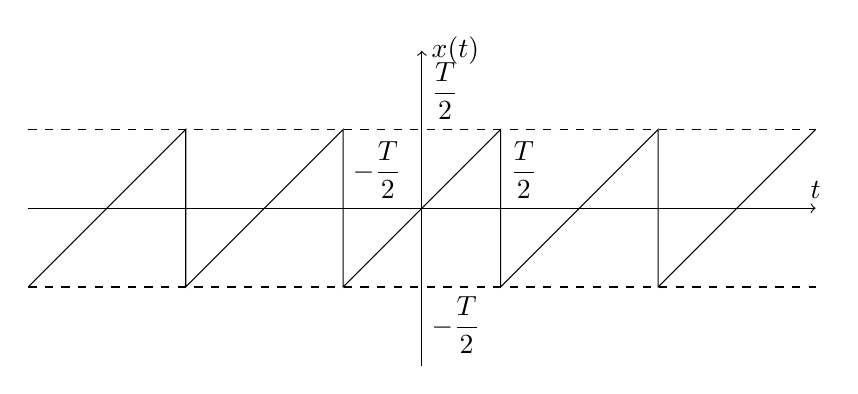
\begin{tikzpicture}[scale=2]
        \draw[->](-2.5,0)--(2.5,0)node[above]{$t$};
        \draw[->](0,-1)--(0,1)node[right]{$x(t)$};
        \draw[-](-2.5,-0.5)--(-1.5,0.5)--(-1.5,-0.5)--(-0.5,0.5)--(-0.5,0)node[above right]{$\displaystyle-\frac{T}{2}$}--(-0.5,-0.5)--(0.5,0.5)--(0.5,0)node[above right]{$\displaystyle\frac{T}{2}$}--(0.5,-0.5)--(1.5,0.5)--(1.5,-0.5)--(2.5,0.5);
        \draw[dashed](-2.5,0.5)--(0,0.5)node[above right]{$\displaystyle\frac{T}{2}$}--(2.5,0.5);
        \draw[dashed](-2.5,-0.5)--(0,-0.5)node[below right]{$-\displaystyle\frac{T}{2}$}--(2.5,-0.5);
    \end{tikzpicture}
\end{center}


Si calcolano i coefficienti di Fourier tramite la definizione, e si calcola l'integrale per parti: 
\begin{gather*}
    c_k=\displaystyle\frac{1}{T}\int_{-\frac{T}{2}}^{\frac{T}{2}}te^{-i\frac{2\pi kt}{T}}dt=\displaystyle\left[-\frac{1}{T}\frac{T}{2i\pi k}te^{-i\frac{2\pi kt}{T}}\right]_{-\frac{T}{2}}^{\frac{T}{2}}-
    \frac{1}{T}\int_{-\frac{T}{2}}^{\frac{T}{2}}-\frac{T}{2i\pi k}e^{-i\frac{2\pi kt}{T}dt}\\
    \displaystyle-\frac{T}{2i\pi k}\left(\frac{e^{-i\pi k}+e^{i\pi k}}{2}\right)+\frac{1}{2i\pi k}\left[\frac{T}{2i\pi k}e^{-i\frac{2\pi kt}{T}}\right]_{-\frac{T}{2}}^{\frac{T}{2}}\\
    \displaystyle-\frac{T}{2i\pi k}\left(\frac{e^{i(-\pi k)}+e^{-i(-\pi k)}}{2}\right)-\frac{2iT}{4\pi^2k^2}\left(\frac{e^{i(-\pi k)}-e^{-i(-\pi k)}}{2i}\right)\\
    \displaystyle-\frac{T}{2i\pi k}\cos\left(-\pi k\right)+\frac{2iT}{4\pi^2k^2}\sin(-\pi k)
\end{gather*}
La componente sinusoidale è nulla per ogni valore di $k$, per cui il coefficiente generico si esprime come:
\begin{gather*}
    c_k=\displaystyle-\frac{T}{2i\pi k}\cos(-\pi k)=\frac{Ti}{2\pi k}\cos(\pi k)=\frac{Ti}{2\pi k}(-1)^k
\end{gather*}
Il coefficiente $c_0$ è nullo, poiché rappresenta il valor medio del periodo. In questo caso essendo un segnale dispari, il valor medio nel periodo è nullo:
\begin{equation*}
    c_0=\displaystyle\frac{1}{T}\int_{-\frac{T}{2}}^{\frac{T}{2}}t\,dt=0
\end{equation*}

Dato il seguente segnale dente di sega:
\begin{center}
    \begin{tikzpicture}[scale=2]
        \draw[->](-3,-0.5)--(2,-0.5)node[above]{$t$};
        \draw[->](-0.5,-1.25)--(-0.5,0.75)node[right]{$x(t)$};
        \draw[-](-2.5,-0.5)--(-1.5,0.5)--(-1.5,-0.5)--(-0.5,0.5)--(-0.5,0)--(-0.5,-0.5)--(0.5,0.5)--(0.5,0)--(0.5,-0.5)node[below right]{$T$}--(1.5,0.5)--(1.5,-0.5);
        \draw[dashed](-3,0.5)--(0,0.5)node[above right]{$T$}--(2,0.5);
    \end{tikzpicture}
\end{center}
Si può esprimere come il precedente segnale analizzato, traslato nel tempo e nello spazio di uno stesso fattore $T/2$. La traslazione nello spazio può essere sia un ritardo 
che un anticipo, poiché si ottiene lo stesso segnale risultante:
\begin{equation*}
    y(t)=x\left(t\pm\frac{T}{2}\right)+\displaystyle\frac{T}{2}
\end{equation*}
Si considera in questo caso un ritardo di $T/2$. Conoscendo i coefficienti di $c_k$, si può attuare una traslazione nel tempo, per ottenere i coefficienti della serie di Fourier 
del segnale $y$:
\begin{gather*}
    d_k=\begin{cases}
        \displaystyle c_0+\frac{T}{2}=\frac{T}{2} &k=0\\
        c_ke^{-i\frac{2\pi k}{T}\frac{T}{2}}=\displaystyle\frac{T}{2i\pi k}(-1)^ke^{-i\pi k}&k\neq0
    \end{cases}
\end{gather*}



Dato un segnale treno di triangoli:
\begin{equation*}
    x(t)=\displaystyle\sum_{k=-\infty}^{+\infty}\mbox{tri}\left(\frac{2(t-kT)}{\tau}\right)
\end{equation*}
\begin{center}
    \begin{tikzpicture}[scale=2]
        \draw[->](-2.5,0)--(2.5,0)node[above]{$t$};
        \draw[->](0,-0.5)--(0,1.5)node[right]{$x(t)$};

        \draw[-](-2,0)--(-1.5,1)--(-1,0)--(-0.5,0)node[below]{$\displaystyle-\frac{\tau}{2}$}--(0,1)node[above right]{$T$}--(0.5,0)node[below]{$\displaystyle\frac{\tau}{2}$}--(1,0)--(1.5,1)--(2,0);
        \draw[dashed](-2.5,1)--(2.5,1);
    \end{tikzpicture}
\end{center}
Si calcolano i coefficienti tramite la definizione. Poiché è presente un solo triangolo nell'intervallo di intergrazione, si può restringere l'intervallo: 
\begin{gather*}
    c_k=\displaystyle\frac{1}{T}\int_{-\frac{T}{2}}^{\frac{T}{2}}\mbox{tri}\left(\frac{2t}{\tau}\right)e^{-i\frac{2\pi kt}{T}}dt=\frac{1}{T}\int_{-\frac{\tau}{2}}^{\frac{\tau}{2}}\left(1-\left|\frac{2t}{\tau}\right|\right)e^{-i\frac{2\pi kt}{T}}dt\\
    \displaystyle\frac{1}{T}\int_{-\frac{\tau}{2}}^{\frac{\tau}{2}}e^{-i\frac{2\pi kt}{T}}dt+\frac{1}{T}\int_{-\frac{\tau}{2}}^{\frac{\tau}{2}}-\left|\frac{2t}{\tau}\right|e^{-i\frac{2\pi kt}{T}}dt\\
    \displaystyle\frac{1}{T}\int_{-\frac{\tau}{2}}^{\frac{\tau}{2}}e^{-i\frac{2\pi kt}{T}}dt-\frac{1}{T}\left(\int_{-\frac{\tau}{2}}^{0}-\frac{2t}{\tau}e^{-i\frac{2\pi kt}{T}}dt+\int_{0}^{\frac{\tau}{2}}\frac{2t}{\tau}e^{-i\frac{2\pi kt}{T}}dt\right)
\end{gather*}
Il primo integrale corrisponde all'integrale ai coefficienti di una finestra, ed è stato già precedentemente calcolato, per cui si omette la risoluzione. Si considera la 
sostituzione $t=-t'$ nel secondo integrale:
\begin{gather*}
    \displaystyle\frac{\tau}{T}\mbox{sinc}\left(\frac{\tau k}{T}\right)-\frac{1}{T}\left(\int_{-\frac{-\tau}{2}}^{0}-\frac{2(-t)}{\tau}e^{-i\frac{2\pi k(-t)}{T}}d(-t)+\int_{0}^{\frac{\tau}{2}}\frac{2t}{\tau}e^{-i\frac{2\pi kt}{T}}dt\right)\\
    \displaystyle\frac{\tau}{T}\mbox{sinc}\left(\frac{\tau k}{T}\right)-\frac{1}{T}\left(-\int_{\frac{\tau}{2}}^{0}\frac{2t}{\tau}e^{i\frac{2\pi kt}{T}}dt+\int_{0}^{\frac{\tau}{2}}\frac{2t}{\tau}e^{-i\frac{2\pi kt}{T}}dt\right)\\
    \displaystyle\frac{\tau}{T}\mbox{sinc}\left(\frac{\tau k}{T}\right)-\frac{1}{T}\left(\int^{\frac{\tau}{2}}_{0}\frac{2t}{\tau}e^{i\frac{2\pi kt}{T}}dt+\int_{0}^{\frac{\tau}{2}}\frac{2t}{\tau}e^{-i\frac{2\pi kt}{T}}dt\right)\\
    \displaystyle\frac{\tau}{T}\mbox{sinc}\left(\frac{\tau k}{T}\right)-\frac{1}{T}\int^{\frac{\tau}{2}}_{0}\frac{4t}{\tau}\frac{e^{i\frac{2\pi kt}{T}}+e^{-i\frac{2\pi kt}{T}}}{2}dt\\
    \displaystyle\frac{\tau}{T}\mbox{sinc}\left(\frac{\tau k}{T}\right)-\frac{4}{\tau T}\int_{0}^{\frac{\tau}{2}}t\cos\left(\frac{2\pi kt}{T}\right)dt
\end{gather*}
Quest'ultimo integrale così ottenuto si risolve mediante integrazione per parti:
\begin{gather*}
    \displaystyle\frac{\tau}{T}\mbox{sinc}\left(\frac{\tau k}{T}\right)-\frac{4}{\tau T}\left[\frac{T}{2\pi k}t\sin\left(\frac{2\pi kt}{T}\right)\right]^{\frac{\tau}{2}}_0
    +\frac{4}{\tau T}\int_{0}^{\frac{\tau}{2}}\frac{T}{2\pi k}\sin\left(\frac{2\pi kt}{T}\right)dt\\
    \displaystyle\frac{\tau}{T}\mbox{sinc}\left(\frac{\tau k}{T}\right)-\frac{\tau}{T}\frac{T}{\pi k\tau}\sin\left(\frac{\pi k\tau}{T}\right)+0+
    \frac{4}{\tau T}\left[-\left(\frac{T}{2\pi k}\right)^2\cos\left(\frac{2\pi kt}{T}\right)\right]^{\frac{\tau}{2}}_0\\
    \displaystyle\frac{\tau}{T}\mbox{sinc}\left(\frac{\tau k}{T}\right)-\displaystyle\frac{\tau}{T}\mbox{sinc}\left(\frac{\tau k}{T}\right)-
    \frac{T}{\pi^2k^2\tau}\left[\cos\left(\frac{\pi k\tau}{T}\right)-1\right]\\
    \displaystyle\frac{2T}{\pi^2k^2\tau}\sin^2\left(\frac{\pi kt}{2T}\right)=
    \frac{\tau}{2T}\left[\frac{2T}{\pi k\tau}\sin\left(\frac{\pi kt}{2T}\right)\right]\left[\frac{2T}{\pi k\tau}\sin\left(\frac{\pi kt}{2T}\right)\right]\\
    c_k=\displaystyle\frac{\tau}{2T}\mbox{sinc}^2\left(\frac{k\tau }{2T}\right)
\end{gather*}
I coefficienti di un treno di triangoli risultano essere dei seni cardinali quadrati. 

\section{Traformata di Fourier}
Quando si trattano segnali non periodici, non si possono esprimere mediante una serie di Fourier, quindi si analizzano mediante la trasformata di Fourier. 
La trasformata di Fuorier si può applicare solamente a segnali impulsivi. Segnali impulsivi sono definiti dalla seguente espressione:
\begin{equation*}
    \displaystyle\int_{-\infty}^{+\infty}|x(t)|dt\neq\infty
\end{equation*}
Come la serie di Fourier la trasformata di Fourier è uno strumento per analizzare i segnali. Questi segnali possono essere nel dominio del tempo $x(t)$ o dominio 
della frequenza $X(f)$. La trasformata è quindi un funzionale che dipende dalla variabile della frequenza, non più dalla variabile del tempo del segnale originale $x(t)$. 
La trasformata $X(f)$ è univoca per ogni segnale $x(t)$ nel tempo. Questa trasformata assoccia univocamente un segnale nel dominio del tempo ad un segnale nel dominio della 
frequenza:   
\begin{equation*}
    \mathscr{F}\{x(t)\}=X(f)
\end{equation*}

Ricordando la serie di un segnale periodico $x$ di periodo $T$:
\begin{gather*}
    x(t)=\displaystyle\sum_{k=-\infty}^{+\infty}c_ke^{i\frac{2\pi kt}{T}}
\end{gather*}
Nello spazio vettoriale dei segnali periodico è stato definito il prodotto scalare:
\begin{equation*}
    \langle x_1(t),\;x_2(t)\rangle=\displaystyle\frac{1}{T}\int_{-\frac{T}{2}}^{\frac{T}{2}}x_1(t)x_2^*(t)dt
\end{equation*}
Nello spazio vettoriale di Fourier, la base ortonormale è formata da tutte le armonica:
\begin{gather*}
    \langle e^{i\frac{2\pi kt}{T}},\;e^{i\frac{2\pi nt}{T}}\rangle=\begin{cases}
        0&\forall k\neq n\\
        1&\forall k=n
    \end{cases}
\end{gather*} 
Da queste armoniche si può ricavare il coefficiente di ordine $k$ di un qualsiasi segnale periodico di periodo $T$:
\begin{equation*}
    c_k=\displaystyle\frac{1}{T}\int_{-\frac{T}{2}}^{\frac{T}{2}}x(t)e^{-i\frac{2\pi kt}{T}}dt
\end{equation*}



Si considerareranno per semplicità tutti i segnali trattati come impulsivi. Per cui non sarà necessario dimostrare l'esistenza della trasformata di un certo segnale $x(t)$ 
non necessariamente periodico. Si vuole rappresentare questo segnale in modo equivalente alla serie di Fourier. Per rappresentare questo segnale sono necessarie un numero 
infinito non numerabile di armoniche, per cui si considera un integrale, dove il coefficiente dipende dalla varibile dell'integrale. E l'armonica non dipende dal parametro 
$k$, ma dalla stessa variabile dell'integrale:
\begin{equation*}
    x(t)=\displaystyle\int_{-\infty}^{+\infty}X(f)e^{2i\pi tf}df
\end{equation*}
Il segnale si esprime quindi tramite un insieme infinito non numerabile di armoniche, sempre uguali per ogni segnale. Per cui la differenza tra due segnali, come per 
l'espansione di Fourier, è il peso di ogni armonica $X(f)$. Bisogna comunque dimostrare che queste armoniche siano una base ortonormale in questo spazio di Fourier. Si 
introduce il prodotto scalare nello spazio dei segnali impulsivi:
\begin{equation*}
    \langle x_1(t),\;x_2(t)\rangle=\displaystyle\int_{-\infty}^{+\infty}x_1(t)x_2^*(t)dt
\end{equation*}
Questo prodotto scalare corrisponde alla correlazione tra due segnali a ritardo nullo. 

Per determinare se due armoniche di frequenze diverse $f_1$ e $f_2$ sono una base si considera il loro prodotto scalare:
\begin{gather*}
    \langle e^{2i\pi f_1t},\;e^{2i\pi f_2t}\rangle=\displaystyle\lim_{\Delta t\to\infty}\int_{-\frac{\Delta t}{2}}^{+\frac{\Delta t}{2}}e^{2i\pi f_1t}e^{-2i\pi f_2t}dt\\
    \displaystyle\lim_{\Delta t\to\infty}\left[\frac{e^{2i\pi(f_1-f_2)t}}{2i\pi(f_1-f_2)}\right]^{\frac{\Delta t}{2}}_{-\frac{\Delta t}{2}}=
    \Delta t\frac{\sin(\pi(f_1-f_2)\Delta t)}{\pi(f_1-f_2)\Delta t}\\
    \displaystyle\lim_{\Delta t\to\infty}\Delta t\,\mbox{sinc}(\Delta t(f_1-f_2))
\end{gather*}
Per $\Delta t\to\infty$, la sinc diventa un impulso tempo continuo:
\begin{equation*}
    \langle e^{2i\pi f_1t},\;e^{2i\pi f_2t}\rangle=\delta(f_1-f_2)
\end{equation*}
Per cui tutte le armoniche di frequenza diversa hanno prodotto scalare nullo, e solo due armoniche di frequenza uguale hanno prodotto scalare di valore unitario. 
Bisogna dimostrare che i coefficienti trasformata di Fourier $X(f)$ si ottengono analogamente ai coefficienti $c_k$:
\begin{gather*}
    X(f)=\langle x(t),\;e^{2i\pi ft}\rangle=\displaystyle\int_{-\infty}^{+\infty}x(t)e^{-2i\pi ft}dt
\end{gather*}
Nello spazio di Fourier si può poi analizzare la banda di un segnale, ovvero il contenuto informativo rispetto alla frequenza. Quest'informazione è necessaria per poter 
trasmettere un determinato segnale. I due domini del tempo e della frequenza sono due domini separati. 
Il nucleo o kernel della trasformata di Fourier corrisponde all'armonica, ovvero il componente esponenziale complesso nell'integrale. 

\subsection{Trasformate Elementari}

Dato un segnale finestra:
\begin{gather*}
    x(t)=\mbox{rect}\displaystyle\left(\frac{t}{\tau}\right)\\
    X(f)=\displaystyle\int_{-\infty}^{+\infty}\mbox{rect}\left(\frac{t}{\tau}\right)e^{-2i\pi ft}dt=\left[\frac{e^{-2i\pi ft}}{2i\pi ft}\right]^{+\frac{\tau}{2}}_{-\frac{\tau}{2}}\\
    \displaystyle\frac{e^{-i\pi f\tau}-e^{-i\pi f\tau}}{-2i\pi f}=\frac{\sin(\pi f\tau)}{\pi f}=\tau\,\mbox{sinc}(f\tau)
\end{gather*}
Quidni la trasfromata di un segnale fienstra di base $\tau$ è un seno cardinale moltiplicato per la base, di argomento moltiplicato per la base:
\begin{gather*}
    x(t)=\mbox{rect}\displaystyle\left(\frac{t}{\tau}\right)\rightarrow X(f)=\tau\,\mbox{sinc}(f\tau)
\end{gather*}
La trasformata in $f=0$, corrisponde al valore medio del segnale finestra:
\begin{equation*}
    X(0)=\displaystyle\int_{-\frac{\tau}{2}}^{\frac{\tau}{2}}dt=\tau
\end{equation*}
%% grafo
Questa proprietà si chiama teormea del valor medio. Ovvero per ogni segnale $x$, la trasformata per la frequenza nulla $f=0$ corrisponde al valore medio del segnale. 



Dato un segnale impulso di Dirac:
\begin{gather*}
    x(t)=\delta(t)\\
    X(f)=\displaystyle\int_{-\infty}^{+\infty}\delta(t)e^{-2i\pi ft}dt=1
\end{gather*}
Per la proprietà di campionamento dell'impulso e per l'area dell'impulso, si ottiene che la trasformata di Fourier dell'impulso è sempre costante è unitario per ogni frequenza. 


Tanto più è limitato nel tempo, tanto più è largo il contenuto spettrale o la banda del segnale. Dove lo spettro di un segnale indica la sua trasformata di Fourier 
$\mathscr{F}$. 


Dato un segnale costante:
\begin{gather*}
    x(t)=1\\
    X(f)=\displaystyle\int_{-\infty}^{+\infty}e^{-2i\pi ft}dt=\delta (f)
\end{gather*}
Analogamente al prodotto scalare tra due armoniche. 
Tanto più p esteso un segnale nel dominio del tempo, tanto più è limitato nel domino della frequenza. 


Dato il segnale impulso traslato:
\begin{gather*}
    x(t)=\delta (t-t_0)\\
    X(f)=\displaystyle\int_{-\infty}^{+\infty}\delta(t-t_0)e^{-2i\pi ft}dt=e^{-2i\pi ft_0}
\end{gather*}
Dato il segnale armonica di frequenza $f_0$:
\begin{gather*}
    x(t)=e^{2i\pi f_0t}\\
    X(f)=\displaystyle\int_{-\infty}^{+\infty}e^{2i\pi(f_0-f)t}dt=\delta(f_0-f)
\end{gather*}
Analogamente al prodotto scalare tra due armoniche di frequenza diversa. 


Dato il segnale coseno:
\begin{gather*}
    x(t)=\cos(2\pi f_0t)\\
    X(f)=\displaystyle\frac{1}{2}\int_{-\infty}^{+\infty}\left(e^{2i\pi f_0t}+e^{-2i\pi f_0t}\right)e^{-2i\pi ft}dt=\frac{\delta(f-f_0)+\delta(f+f_0)}{2}\\
    x(t)=\cos(2\pi f_0t)\rightarrow X(f)=\displaystyle\frac{\delta(f-f_0)+\delta(f+f_0)}{2}
\end{gather*}
Nella notazione di Fourier un coseno viene rappresentato come due frequenze $\pm f_0$. 
Analogamente per il seno:
\begin{gather*}
    x(t)=\sin(2\pi f_0t)\\
    X(f)=\displaystyle\int_{-\infty}^{+\infty}\frac{1}{2i}(e^{2i\pi f_0t}-e^{-2i\pi f_0t})e^{-2i\pi ft}dt=\frac{\delta (f-f_0)-\delta(f+f_0)}{2i}
\end{gather*}
Dato un coseno di ampiezza $A$ con un anticipo di fase $\phi$: 
\begin{gather*}
    x(t)=A\cos(2\pi f_0t+\phi)\\
    X(f)=\displaystyle\frac{A}{2}\int_{-\infty}^{+\infty}\left(e^{2i\pi f_0t}e^{i\phi}+e^{-2i\pi f_0t}e^{-i\phi}\right)e^{-2i\pi ft}dt\\
    X(f)=\frac{A\delta(f-f_0)e^{i\phi}+A\delta(f+f_0)e^{-i\phi}}{2}
\end{gather*}

\subsection{Proprietà di Linearità}

La trasformata di Fourier è un operatore linerae. Dati due segnali $x(t)$ e $y(t)$:
\begin{gather*}
    x(t)\to X(f)\\
    y(t)\to Y(f)\\
    ax(t)+by(t)=\displaystyle\int_{-\infty}^{+\infty}(ax(t)+by(t))e^{-2i\pi ft}dt\\
    a\int_{-\infty}^{+\infty}x(t)e^{-2i\pi ft}dt+b\int_{-\infty}^{+\infty}y(t)e^{-2i\pi ft}dt= 
    aX(f)+bY(f)
\end{gather*}

\subsection{Proprietà di Dualità}

La trasformata di Fourier accoppia due segnali nei due domini. Se la trasformata di un segnale $x$ nel tempo è una funzione $y$ nella frequenza, la trasfromata di un segnale $y$ 
nel tempo è un segnale $x$ nella frequenza, di variabile opposta $-f$.

Per dimostrare questa prorpietà si considerano la formula di trasformazione:
\begin{equation*}
    X(f)=\displaystyle\int_{-\infty}^{+\infty}x(t)e^{-2i\pi ft}dt
\end{equation*}
E la formula di antitrasformazione:
\begin{equation*}
    x(t)=\displaystyle\int_{-\infty}^{+\infty}X(f)e^{2i\pi ft}df
\end{equation*}

Data la trasformata di un segnale $x(t)$ $X(f)$, per riportarla nel dominio del tempo, si considera l'integrale di trasformazione di $X(t)$:
\begin{gather*}
    \displaystyle\int_{-\infty}^{+\infty}X(t)e^{-2i\pi ft}dt
\end{gather*}
Si considera la sotituzione $f=t'$ e $t=f'$, l'integrale diventa l'integrale di antitrasformazione:
\begin{equation*}
    \displaystyle\int_{-\infty}^{+\infty}X(f')e^{-2i\pi f't'}df'=x(-t')
\end{equation*}
Allora:
\begin{gather*}
    \mathscr{F}\{x(t)\}= X(f)\\
    \mathscr{F}\{X(t)\}=x(-f)
\end{gather*}

\subsection{Proprietà di Scala}

Si considera la trasformata di un segnale:
\begin{gather*}
    x(at)\to\displaystyle\int_{-\infty}^{+\infty}x(at)e^{-2i\pi ft}dt\\
    t'=at\\
    \displaystyle\frac{1}{a}\int_{-\infty}^{+\infty}x(t')e^{-2i\pi \frac{f}{a}t'}dt'=\frac{1}{a}X\left(\frac{f}{a}\right)
\end{gather*}
Se $a=-1$, la trasformata corrisponde a:
\begin{gather*}
    \displaystyle\int_{-\infty}^{+\infty}x(-t)e^{-2i\pi ft}dt\\
    t'=-t\\
    \displaystyle\int_{-\infty}^{+\infty}x(t')e^{-2i\pi(- f)t'}dt'=X(-f)
\end{gather*}
Per cui quando $a<0$:
\begin{gather*}
    x(at)\to\displaystyle\int_{-\infty}^{+\infty}x(t)e^{-2i\pi ft}dt\\
    t'=at\\
    \displaystyle\frac{1}{|a|}\int_{-\infty}^{+\infty}x(t')e^{-2i\pi \left(-\frac{f}{a}\right)t'}dt'=\frac{1}{|a|}X\left(-\frac{f}{a}\right)
\end{gather*}
Per cui in generale dato un segnale scalato di un fattore $a$, la sua trasformata è:
\begin{gather*}
    \mathscr{F}\{x(at)\}=\displaystyle\frac{1}{|a|}X\left(\frac{f}{a}\right)
\end{gather*}

\subsection{Altre Trasformate Elementari}

Si considera la trasformata del segnale gaussiano:
\begin{gather*}
    x(t)=e^{-\alpha t^2}\\
    X(f)=\displaystyle\int_{-\infty}^{+\infty}e^{-\alpha t^2}e^{-2i\pi ft}dt=\int_{-\infty}^{+\infty}e^{-\alpha\left(\frac{2i\pi ft}{\alpha} + t^2\right)}dt\\
    \displaystyle\int_{-\infty}^{+\infty}e^{-\alpha\left[t^2+\frac{2i\pi ft}{\alpha}+\left(\frac{i\pi f}{\alpha}\right)^2-+\left(\frac{i\pi f}{\alpha}\right)^2\right]}dt\\
    e^{-\frac{\pi^2f^2}{\alpha}}\displaystyle\int_{-\infty}^{+\infty}e^{-\alpha\left(t+\frac{i\pi f}{\alpha}\right)^2}dt
\end{gather*}
Si applica la sotituzione $\tau=\sqrt{\alpha}(t+i\pi f/\alpha)$, l'integrale diventa allora:
\begin{gather*}
    e^{-\frac{\pi^2f^2}{\alpha}}\displaystyle\int_{-\infty}^{+\infty}e^{-\tau^2}\frac{d\tau}{\sqrt{\alpha}}=e^{-\frac{\pi^2f^2}{\alpha}}\sqrt{\frac{\pi}{\alpha}}\\
    X(f)=\sqrt{\frac{\pi}{\alpha}}e^{-\frac{\pi^2f^2}{\alpha}}
\end{gather*}

In forma normalizzata la gaussiana si esprime direttamente rispetto alla deviazione standard $\sigma$ e alla sua varianza $\sigma^2$:
\begin{gather*}
    x(t)=e^{-\frac{t^2}{2\sigma^2}}\\
    X(f)=\sqrt{2\pi}\sigma e^{-2\pi^2\sigma^2f^2}
\end{gather*}
L'area sottesa dalla gaussiana risulta essere il valor medio, esprimibile tramite la 
\begin{equation*}
    X(0)=\sqrt{2\pi}\sigma
\end{equation*}
La gaussiana è una delle pochissime funzioni che si autotrasforma. 

Si determina la trasformata dell'esponenziale unilatero:
\begin{gather*}
    x(t)=e^{-\alpha t}u(t)\\
    X(f)=\displaystyle\int_{-\infty}^{+\infty}e^{-\alpha t}u(t)e^{-2i\pi ft}dt=\int_0^{+\infty}e^{-(2i\pi f+\alpha)t}dt\\
    \left[\displaystyle\frac{e^{-(2i\pi f+\alpha)t}}{-(\alpha+2i\pi f)}\right]^{+\infty}_0=0+\frac{1}{\alpha+2i\pi f}\\
    X(f)=\frac{1}{\alpha+ 2i\pi f}
\end{gather*}
Il modulo quadro del segnale corrisponde ad una Lorentziana, una funzione simile ad una gaussiana: 
\begin{equation*}
    \left|X(f)\right|^2=\frac{1}{\alpha^2+4\pi^2f^2}
\end{equation*}
\begin{center}
    \begin{tikzpicture}[scale=2]
        \draw[->](-1.5,0)--(1.5,0)node[above right]{$f$};
        \draw[->](0,-0.5)--(0,1.5)node[right]{$X(f)$};

        \draw[-]plot[smooth, domain=-1.5:1.5](\x,{1/(2*(\x)^2+1)});
    \end{tikzpicture}
\end{center}


Dato il segnale esponenziale del modulo. Si può esprimere il segnale come due esponenziali unilateri:
\begin{center}
    \begin{tikzpicture}[scale=2]
        \draw[->](-1.5,0)--(1.5,0)node[above]{$f$};
        \draw[->](0,-0.5)--(0,1.5)node[right]{$X(f)$};

        \draw[-]plot[smooth, domain=0:1.5](\x,{e^(-2*(\x))});
        \draw[-]plot[smooth, domain=-1.5:0](\x,{e^(2*(\x))});
    \end{tikzpicture}
\end{center}
\begin{gather*}
    x_1(t)=e^{-\alpha|t|}\\
    x_1(t)=x(t)+x(-t)\\
    X_1(f)=X(f)+X(-f)=\displaystyle\frac{1}{\alpha+2i\pi f}+\frac{1}{\alpha-2i\pi ft}=\frac{2\alpha}{\alpha^2+4\pi^2f^2}
\end{gather*}
Per cui la sua trasformata corrisponde alla Lorentziana. 


Dato il segnale Lorentziana, si può calcolare la sua trasformata tramite la proprietà di dualità della trasformata: 
\begin{gather*}
    x_2(t)=\displaystyle\frac{1}{\alpha+2i\pi t}\\
    X(f)=x(-f)=e^{\alpha f}u(-f)
\end{gather*}



Dato il segnale gradino, si può esprimere come il limite di un esponenziale unilatero:
\begin{equation*}
    x_3(t)=u(t)=\lim_{\alpha\to0}e^{-\alpha t}{u(t)}
\end{equation*}
Poiché non è un segnale impulsivo, questo risultato non rappresenta la trasformata su tutte le frequenza. 
\begin{gather*}
    X(f)=\displaystyle\lim_{\alpha\to0}\frac{1}{\alpha+2i\pi f}=\frac{1}{2i\pi f}
\end{gather*}
Razionalizzando l'argomento del limite si osserva come il risultato ottenuto per frequenze nulle perda informazioni sulla trasformata:
\begin{gather*}
    \displaystyle\lim_{\alpha\to0}\frac{1}{\alpha+2i\pi f}=\lim_{\alpha\to0}\left(\frac{\alpha}{\alpha^2+4\pi^2f^2}-\frac{2i\pi f}{\alpha^2+4\pi^2f^2}\right)
\end{gather*}


Per cui si esprime la trasformata di un gradino come il limite ottenuto sommato ad una costante $A$ moltiplicata per l'impulso, per considerare il valore della trasformata 
per frequenze nulle: 
\begin{gather*}
    X(f)=\displaystyle\lim_{\alpha\to0}\frac{1}{\alpha+2i\pi f}=\frac{1}{2i\pi f}+\delta(f)A
\end{gather*}
Il fattore $A$ si ottiene integrando il fattore che si annulla nel limite:
\begin{gather*}
    A=\displaystyle\int_{-\infty}^{+\infty}\frac{\alpha}{\alpha^2+4\pi^2f^2}df=\int_{-\infty}^{+\infty}\frac{1}{\alpha\left(1+\frac{4\pi^2f^2}{\alpha^2}\right)}dt\\
    f'=\displaystyle\frac{2\pi f}{\alpha}\\
    \displaystyle\frac{1}{\alpha}\frac{\alpha}{2\pi}\int_{-\infty}^{+\infty}\frac{1}{1+f'^2}df'=\left[\frac{1}{2\pi}\arctan f'\right]^{+\infty}_{-\infty}=\frac{1}{2\pi}\left[\frac{\pi}{2}-\left(-\frac{\pi}{2}\right)\right]=\frac{1}{2}
\end{gather*}
Per cui la trasofrmata di un gradino, segnale non impulsivo, risulta essere:
\begin{equation*}
    X_3(f)=\displaystyle\frac{1}{2}\delta(f)+\frac{1}{2i\pi f}
\end{equation*}


Si considera il segnale segno, e si vuole determinare la sua trasformata:
\begin{gather*}
    x_4(t)=\mbox{sign}(t)=u(t)-u(-t)\\
    X_4(f)=X_3(f)-X_3(-f)=\displaystyle\frac{1}{2}\delta(f)+\frac{1}{2i\pi f}-\frac{1}{2}\delta(f)+\frac{1}{2i\pi f}=\frac{1}{i\pi f}
\end{gather*}

\subsection{Funzioni di Trasferimento}

Per determinare la risposta impulsiva di un filtro si considera in entrata un impulso, ma inviare un segnale infinitesimo in un sistema non è semplice. Per cui generalmente 
si inserisce in ingresso un armonica a frequenza costante $f_0$:
\begin{gather*}
    y(t)=\displaystyle\int_{-\infty}^{+\infty}h(t)e^{2i\pi f_0(t-\tau)}d\tau\\
    e^{2i\pi f_0t}\displaystyle\int_{-\infty}^{+\infty}h(t)e^{-2i\pi f_0\tau}d\tau=e^{2i\pi f_0t}H(f_0)
\end{gather*}
Si definisce la risposta impulsiva nel dominio della frequenza la funzione di trasferimento del sistema. I filtri sono sistemi che filtrano nel dominio delle frequenze. 

Per cui un filtro è caratterizzato dalla risposta impulsiva o dalla sua funzione di trasferimento, che indica quale frequenze vengono eliminate dal filtro. 




Una Lorentziana è un segnale dove la maggior parte del contenuto informativo è all'interno di un'intervallo finito. Si definiscono quindi dei segnali passa basso, 
ovvero dei sengali il cui contenuto informativo è presente nell'intorno dell'origine. Se un filtro ha funzione di trasferimento passa basso, allora si definisce segnale 
passa basso. La banda del segnale è legata alla frequenza massima $f_{max}$, non è necessario sia una finestra in frequenza, una qualsiasi funzione che assume valori nulli 
per frequenze maggiori della frequenza massima è una funzione passa basso valida per essere funzione di trasferimento di un fitro. 

Tutti i segnali inviati per cavi presentano una banda base, ovvero sono segnali passa basso. 


Esistono altri segnali chiamati passa banda, o modulati. Il segnale è centrato in una frequenza $\pm f_0$, chiamata portante. Si usano per la trasmissioni di segnali 
che vengono inviati nell'etere, tutti questi segnali devono essere modulati. 

\subsection{Traslazione nel Tempo}

Data la trasformata di Fourier di un segnale tempo continuo, è nota anche la trasformata del segnale ritardato o anticipiato:
\begin{gather*}
    \mathscr{F}\{x(t)\}=X(f)\\
    \mathscr{F}\{x(t-t_0)\}=\displaystyle\int_{-\infty}^{+\infty}x(t-t_0)e^{-2i\pi ft}dt\\
    \tau=t-t_0\\
    \displaystyle\int_{-\infty}^{+\infty}x(\tau)e^{-2i\pi f(\tau+t_0)}d\tau=e^{-2i\pi ft_0}\int_{-\infty}^{+\infty}x(\tau)e^{-2i\pi f\tau}d\tau=e^{-2i\pi ft_0}X(f)
\end{gather*}

Data una gaussiana traslata nel tempo:
\begin{gather*}
    x(t)=e^{-\alpha(t-t_0)^2}\\
    X(f)=\displaystyle\sqrt{\frac{\pi}{\alpha}}e^{-\left(\frac{\pi^2f^2}{\alpha}+2i\pi ft_0\right)}
\end{gather*}

\subsection{Traslazione in Frequenza}

Questa proprietà si indica anche come proprietà di modulazione. 
Si considera un segnale moltiplicato per un armonica di frequenza costante $f_0$:
\begin{gather*}
    \mathscr{F}\left\{e^{2i\pi f_0t}x(t)\right\}=\displaystyle\int_{-\infty}^{+\infty}x(t)e^{-2i\pi(f-f_0)t}dt=X(f-f_0)
\end{gather*}

Quest'operazione si chiama modulazione di ampiezza (AM). Il segnale trasmesso cossiponde ad un coseno di ampiezza pari al segnale originario.
\begin{gather*}
    \mathscr{F}\{x(t)\cos(2\pi f_0t)\}=\displaystyle\frac{1}{2}\int_{-\infty}^{+\infty}x(t)\left[e^{2i\pi f_0t}+e^{-2i\pi f_0t}\right]e^{-2i\pi ft}dt\\
    \frac{1}{2}\displaystyle\int_{-\infty}^{+\infty}x(t)e^{-2i\pi(f-f_0)t}dt+\frac{1}{2}\int_{-\infty}^{+\infty}x(t)e^{-2i\pi (f+f_0)t}dt=\frac{X(f-f_0)}{2}+\frac{X(f+f_0)}{2}
\end{gather*}

\subsection{Esercizi sulla Trasformata}

Si considera una finestra di base $T$ moltiplicata per un coseno di frequenza costante $f_0$, ovvero modulata di una frequenza $f_0$:
\begin{gather*}
    x(t)=\mbox{rect}\displaystyle\left(\frac{t}{T}\right)\cos(2\pi f_0t)\\
    \mathscr{F}\{x(t)\}=\frac{T}{2}\mbox{sinc}((f-f_0)T)+\frac{T}{2}\mbox{sinc}\left((f+f_0)T\right)
\end{gather*}
Si considera il seguente segnale:
\begin{center}
    \begin{tikzpicture}[scale=2]
        \draw[->](-1.5,0)--(1.5,0)node[above]{$t$};
        \draw[->](0,-1)--(0,1)node[right]{$x(t)$};
        \draw[-](-1,0)node[below]{$-T$}--(-1,0.5)--(0,0.5)node[right]{$T$}--(0,-0.5)node[left]{$-T$}--(1,-0.5)--(1,0)node[below right]{$T$};
    \end{tikzpicture}
\end{center}

Si vuole calcolare la sua trasformata:
\begin{gather*}
    x(t)=\mbox{rect}\left(\displaystyle\frac{t+T/2}{T}\right)-\mbox{rect}\left(\displaystyle\frac{t-T/2}{T}\right)
\end{gather*}
Per la linearità della trasformata e per la proprietà di traslazione nel tempo la trasformata si ottiene come:
\begin{gather*}
    X(f)=T\left(e^{i\pi fT}-e^{-i\pi fT}\right)\mbox{sinc}\left(T f\right)=2Ti\sin(\pi fT)\mbox{sinc}(Tf)\\
    2iT\displaystyle\frac{\sin(\pi fT)}{\pi fT}\sin(\pi fT)=2i\frac{\sin^2(\pi fT)}{\pi f}
\end{gather*}




\end{document}